\documentclass[kpfonts]{patmorin}
\usepackage{pat}
\usepackage{paralist,graphicx}
\usepackage{array,longtable}

\usepackage[utf8]{inputenc}
\usepackage{todonotes}

\usepackage[noabbrev,capitalise]{cleveref}
\crefname{lem}{Lemma}{Lemmas}
\crefname{thm}{Theorem}{Theorems}
\crefname{cor}{Corollary}{Corollaries}
\crefname{prop}{Proposition}{Propositions}
\crefname{conj}{Conjecture}{Conjectures}
\crefname{open}{Open Problem}{Open Problems}
\crefname{obs}{Observation}{Observations}

\crefformat{equation}{(#2#1#3)}
\Crefformat{equation}{Equation #2(#1)#3}

\usepackage[numbers,sort&compress]{natbib}
\usepackage{hypernat}
\makeatletter
\def\NAT@spacechar{~}
\makeatother

\setlength{\parskip}{1ex}
\setlength{\parindent}{0ex}

\newtheorem{property}{Property}
\newcommand{\plabel}[1]{\label{prop:#1}}
\newcommand{\pref}[1]{Property~\ref{prop:#1}}

\DeclareMathOperator{\sn}{sn}
\DeclareMathOperator{\qn}{qn}
\DeclareMathOperator{\sqn}{sqn}
\DeclareMathOperator{\dsn}{dsn}
\DeclareMathOperator{\tw}{tw}

\renewcommand{\SS}{\mathcal{S}}

\renewcommand{\le}{\leqslant}
\renewcommand{\leq}{\leqslant}
\renewcommand{\ge}{\geqslant}
\renewcommand{\geq}{\geqslant}

\newcommand{\CartProd}{\mathbin{\square}}

\title{\MakeUppercase{Stack-Number is not Bounded by Queue-Number}}

\author{%
	Vida Dujmovi\'c,\!\!%
	\thanks{School of Computer Science and Electrical Engineering,
		University of Ottawa, Ottawa, Canada (\texttt{vida.dujmovic@uottawa.ca}).
		Research supported by NSERC and the Ontario Ministry of Research and Innovation.}
	\,\,
	Robert Hickingbotham,\!\!%
	\thanks{School of Mathematics, Monash University, Melbourne, Australia (\texttt{robert.hickingbotham@monash.edu}).}
	\,\,
	Pat Morin,\!\!%
	\thanks{School of Computer Science, Carleton University, Ottawa, Canada (\texttt{morin@scs.carleton.ca}). Research  supported by NSERC and the Ontario Ministry of Research and Innovation.}
	\,\,
	David R. Wood\thanks{School of Mathematics, Monash University, Melbourne, Australia (\texttt{david.wood@monash.edu}). Research supported by the Australian Research Council.}
}

\begin{document}
\maketitle

\begin{abstract}
We describe a family of graphs with queue-number at most 4 but unbounded stack-number. This resolves open problems of Heath, Leighton and Rosenberg (1992) and Blankenship and Oporwoski (1999).
\end{abstract}

\bigskip

\section{Introduction}

Stacks and queues are fundamental data structures in computer science, but which is more powerful? In 1992, Heath, Leighton and Rosenberg~\cite{HLR92,HR92} introduced an approach for answering this question by defining the graph parameters \textit{stack-number} and \textit{queue-number} (defined below), which respectively measure the power of stacks and queues for representing graphs. The following fundamental problems, implicit in \citep{HLR92,HR92}, were made explicit by \citet{DujWoo05}\footnote{A \emph{graph parameter} is a function $\alpha$ such that $\alpha(G)\in\mathbb{R}$ for every graph $G$, such that $\alpha(G_1)=\alpha(G_2)$ for all isomorphic graphs $G_1$ and $G_2$. A graph parameter $\alpha$ is \textit{bounded} by a graph parameter $\beta$ if there exists a function $f$ such that $\alpha(G) \leq f(\beta(G))$ for every graph $G$.}:
\begin{compactitem}
	\item Is stack-number bounded by queue-number?
	\item Is queue-number bounded by stack-number?
\end{compactitem}

If stack-number is bounded by queue-number but queue-number is not bounded by stack-number, then stacks would be considered to be more powerful than queues. Similarly, if the converse holds, then queues would be considered to be more powerful than stacks. Despite extensive research on stack- and queue-numbers, these fundamental questions have remained unsolved.

We now formally define stack- and queue-number.
Let $G$ be a graph and let $\prec$ be a total order on $V(G)$.  Two disjoint edges $vw,xy\in E(G)$ with $v\prec w$ and $x\prec y$ \emph{cross} with respect to $\prec$ if $v\prec x\prec w\prec y$ or $x\prec v\prec y\prec w$, and \emph{nest} with respect to $\prec$ if $v\prec x\prec y\prec w$ or $x\prec v\prec w\prec y$.
%A set of $k$ pairwise nested edges is called a \emph{$k$-rainbow} and a set of $k$ pairwise crossing edges is called a \emph{$k$-twist}. A set of $k$ edges, no pair of which nest and no pair of which cross is called a \emph{hopper}.
Let $\varphi:E(G)\to\{1,\ldots,k\}$ for some integer $k\ge 1$.  Then $(\prec,\varphi)$ is a \emph{$k$-stack layout} of $G$ if, for every pair of edges $vw,xy\in E(G)$, if $\varphi(vw) = \varphi(xy)$ then $vw$ and $xy$ do not cross.\todo{PM: Suggestion: Replace second if then with $\varphi(vw)\neq\varphi(xy)$ or $vw$ and $xy$ do not cross.} Similarly, the pair $(\prec,\varphi)$ is a \emph{$k$-queue layout} of $G$ if, for every pair of edges $vw,xy\in E(G)$, if $\varphi(vw)=\varphi(xy)$ then  $vw$ and $xy$ do not nest. The smallest integer $s$ for which $G$ has an $s$-stack layout is called the \emph{stack-number} of $G$, denoted  $\sn(G)$. The smallest integer $q$ for which $G$ has a $q$-queue layout is called the \emph{queue-number} of $G$, denoted $\qn(G)$. Note that stack layouts are equivalent to book embeddings (first defined by \citet{Ollmann73}), and stack-number is also known as \emph{page-number}, \emph{book-thickness} or \emph{fixed outer-thickness}. See \citep{BK79,DujWoo04,DujWoo-DCG07,DJMMUW20,DFP13,BFGMMRU19,Yannakakis89,Yann20,MBKPRU20} and the references therein for work on stack- and queue-layouts.

Given a $k$-stack layout $(\prec,\varphi)$ of a graph $G$, for each $i\in\{1,\dots,k\}$, the set $\varphi^{-1}(i)$ behaves like a stack, in the sense that each edge $vw \in \varphi^{-1}(i)$ with $v\prec w$ corresponds to an element in a sequence of stack opertions, such that if we traverse the vertices in the order of $\prec$, then $vw$ is pushed onto the stack at $v$ and popped off the stack at $w$. Similarly, each set $\varphi^{-1}(i)$ in a queue layout  behaves like a queue. In this way, the stack-number and queue-number  respectively measure the power of stacks and queues to represent graphs.


\subsection*{Is Stack-Number Bounded by Queue-number?}

This paper considers the first of the above questions. In a positive direction, \citet{HLR92}  showed that every 1-queue graph has a $2$-stack layout. On the other hand, they described graphs that need exponentially more stacks than queues. In particular, $n$-vertex ternary hypercubes have queue-number $O(\log n)$ and stack-number $\Omega(n^{1/9-\epsilon})$ for any $\epsilon>0$.

%Note that, in an $s$-stack layout, $(\prec,\varphi)$, $\varphi$ is a proper $s$-colouring of the auxilliary graph $H$ with vertex set $V(H)=E(G)$ and in which the edge $ef$ if present if and only if $e$ and $f$ cross with respect to $\varphi$.  Any $k$-twist in $G$ with respect to $\prec$ corresponds to a $k$-clique $H$.  Since the chromatic number of any graph is bounded by its clique number, the following observation is trivial:

%\begin{obs}\obslabel{no-s-twist}
%If $(\prec,\varphi)$ is an $s$-stack layout of a graph $G$ then $E(G)$ does not contain any $k$-twist for any $k>s$.
%\end{obs}

%We now formally define stack and queue layouts of graphs. Let $G=(V,E)$ be a graph with disjoint edges $vw, xy$ and a linear ordering $\leq$ of the vertices. Without loss of generality, we may assume that $v < w$, $x <y$ and $v < x$. We say that $vw$ and $xy$ \textit{cross} if $v<x<w<y$,  \textit{nest} if $v <x <y < w$, and are \textit{disjoint} if $v <w<x<y$. \todo{DW: Do we  need ``disjoint''?} A \textit{stack} is a set of pairwise non-crossing edges and a \textit{queue} is a set of pairwise non-nesting edges. A $k$-queue layout of $G$ consist of a linear ordering $\leq$ of its vertices and a partition $E_1,E_2, \dots, E_k$, of its edges into queues with respect to $\leq$. The stack-number of a graph $G$, $\sn(G)$, is the minimum integer $k$ such that $G$ has a $k$-stack layout. Similarly, the queue-number of a graph $G$, $\qn(G)$, is the minimum integer $k$ such that $G$ has a $k$-queue layout. We note that stack layouts of graphs are related to book embeddings of graph and that stack-number is also known as \textit{page-number}, \textit{book-thickness}, or \textit{fixed outer-thickness}.

%Note that stacks and queues are closely related to breadth-first search (BFS) and depth-first search (DFS) layouts of graphs. It can be easily shown that a BFS vertex ordering of a tree admits a $1$-queue layout and a DFS vertex ordering of a tree admits a $1$-stack layout.

%\citet{HLR92} showed that every 1-queue graph has a 2-stack layout. \citet{HLR92} showed that the ternary hypercubes requires exponentially more stacks than queues. In particular, $n$-vertex ternary hypercubes have queue-number at most $2 \log_3 n$, but stack-number at least $\Omega(n^{1/9-\epsilon})$ for any $\epsilon>0$. We prove the following theorem, which shows that stack-number is not bounded by queue-number.

Our key contribution is the following theorem, which shows that stack-number is not bounded by queue-number. This demonstrates that stacks are not more powerful than queues for representing graphs.

\begin{thm}\label{family}
	%  There exists a family $\mathcal{F}$ of graphs for which $\qn(G)\le 4$ for every $G\in\mathcal{F}$, and for every $s\in\N$, there exists $G\in\mathcal{F}$ for which $\sn(G)>s$.
	For every $s\in \N$ there exists a graph $G$ with $\qn(G)\le 4$ and $\sn(G)>s$.
\end{thm}

As illustrated in \cref{graph}, the graph $G$ in \cref{family} is the cartesian product\footnote{For graphs $G_1$ and $G_2$, the \emph{cartesian product} $G_1\CartProd G_2$ is the graph with vertex set $\{(v_1,v_2): v_1 \in V(G_1), v_2 \in V(G_2)\}$, where $(v_1,v_2)(w_1,w_2)\in E(G_1\CartProd G_2)$ if $v_1=w_1$ and $v_2w_2\in E(G_2)$, or $v_1w_1\in E(G_1)$ and $v_2=w_2$.} $S_b\CartProd H_n$, where $S_b$ is the star graph with root $r$ and $b$ leaves, and $H_n$ is the dual of the hexagonal grid, defined by
\begin{align*}
V(H_n)  :=\{1,\ldots,n\}^2 \quad \text{ and } \quad
E(H_n) & :=  \{(x,y)(x+1,y):x\in\{1,\ldots,n-1\},\,y\in\{1,\ldots,n\}\} \\
& \qquad \cup \{(x,y)(x,y+1):x\in\{1,\ldots,n\},\,y\in\{1,\ldots,n-1\}\} \\
& \qquad \cup \{(x,y)(x+1,y+1):x,y\in\{1,\ldots,n-1\}\} \enspace .
\end{align*}
In \cref{family}, $b$ and $n$ are chosen to be sufficiently large compared to $s$.
%Note that the Hex graph corresponds to the board used in the game \textit{Hex} which was invented by the  Peit Hein in 1942. In this paper, we prove \Cref{family} with the graph $G:= S_b \square H_n$ where $b$ and $n$ are large compared to $s$.
Note that \citet{Pupyrev20} independently suggested using graph products to show that stack-number is not bounded by queue-number.

\begin{figure}[!h]
	\begin{center}
		\begin{tabular}{m{.25\textwidth}m{2ex}m{.25\textwidth}m{2ex}m{.3\textwidth}}
			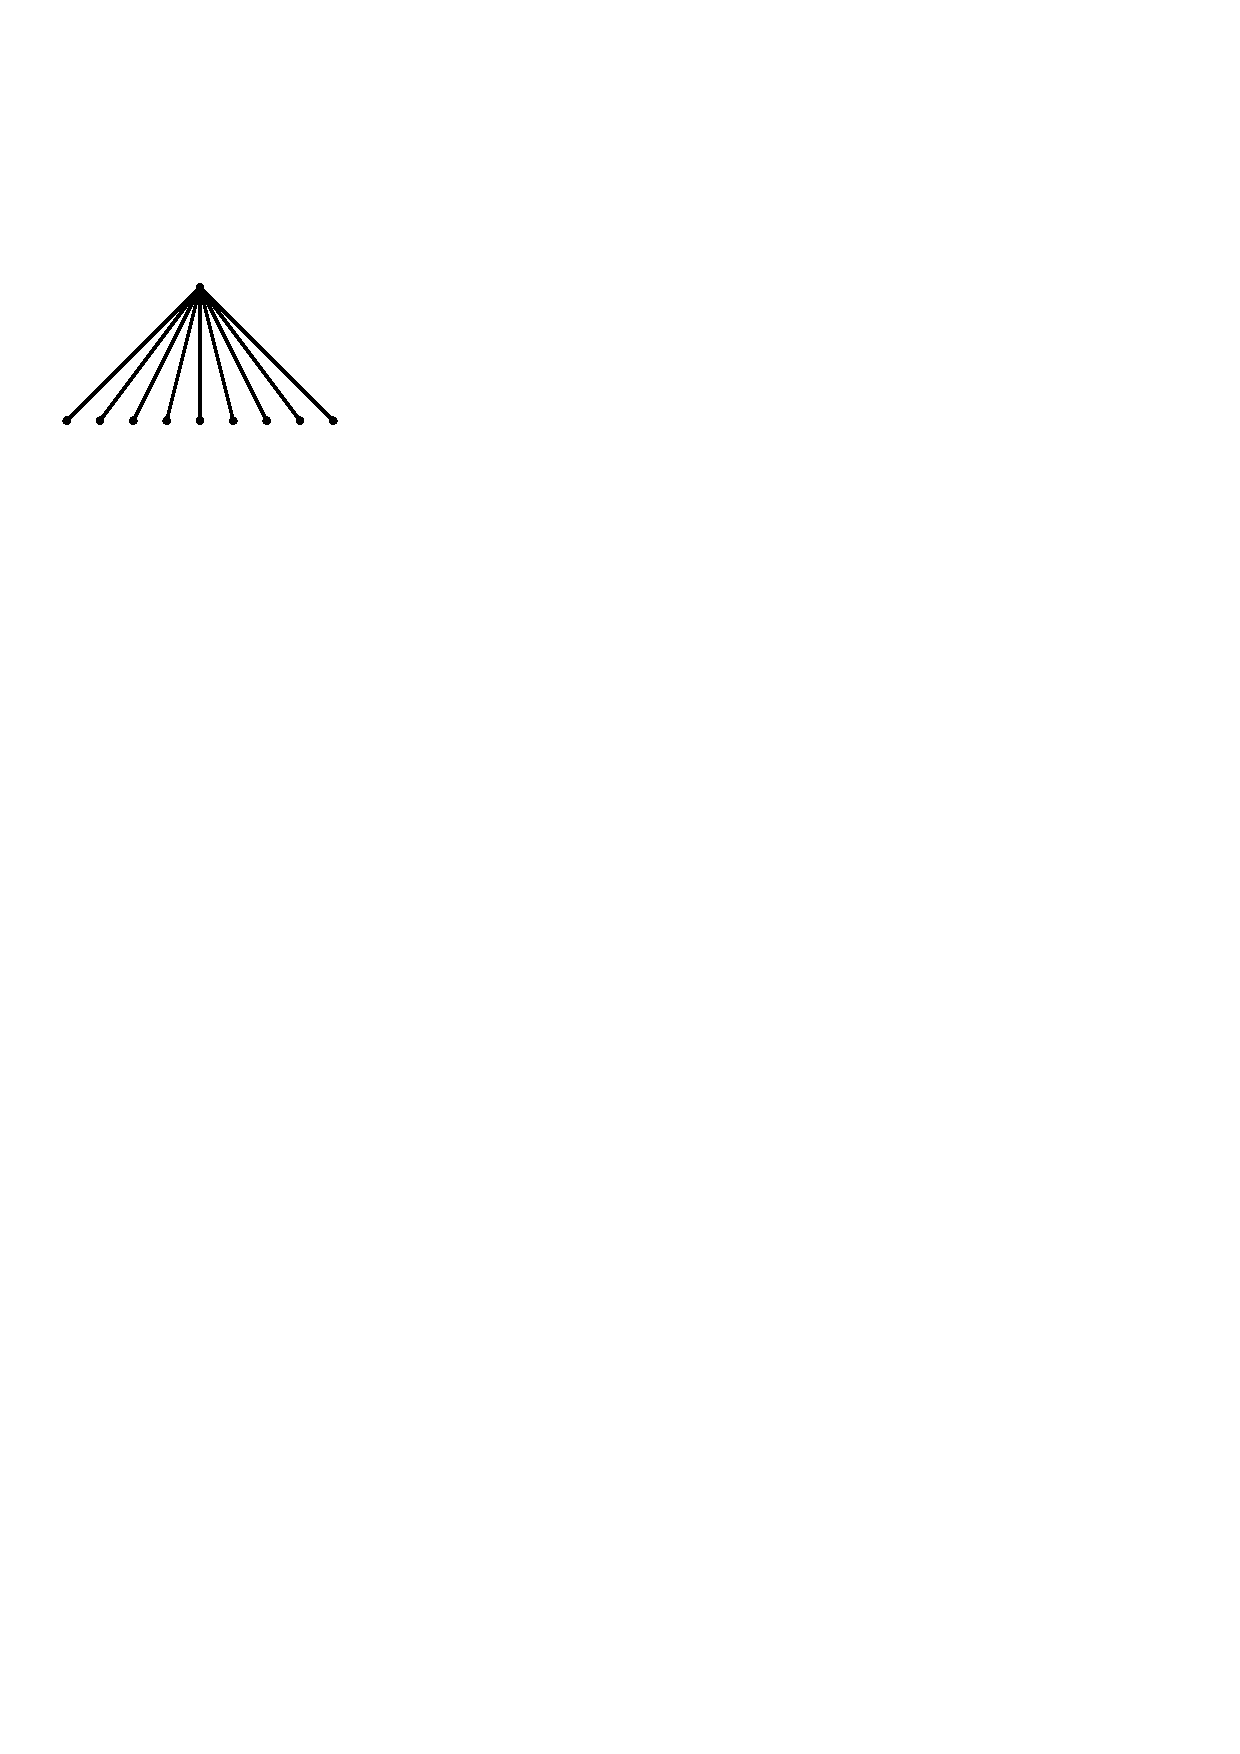
\includegraphics[width=.25\textwidth]{figs/s} & $\CartProd$ & 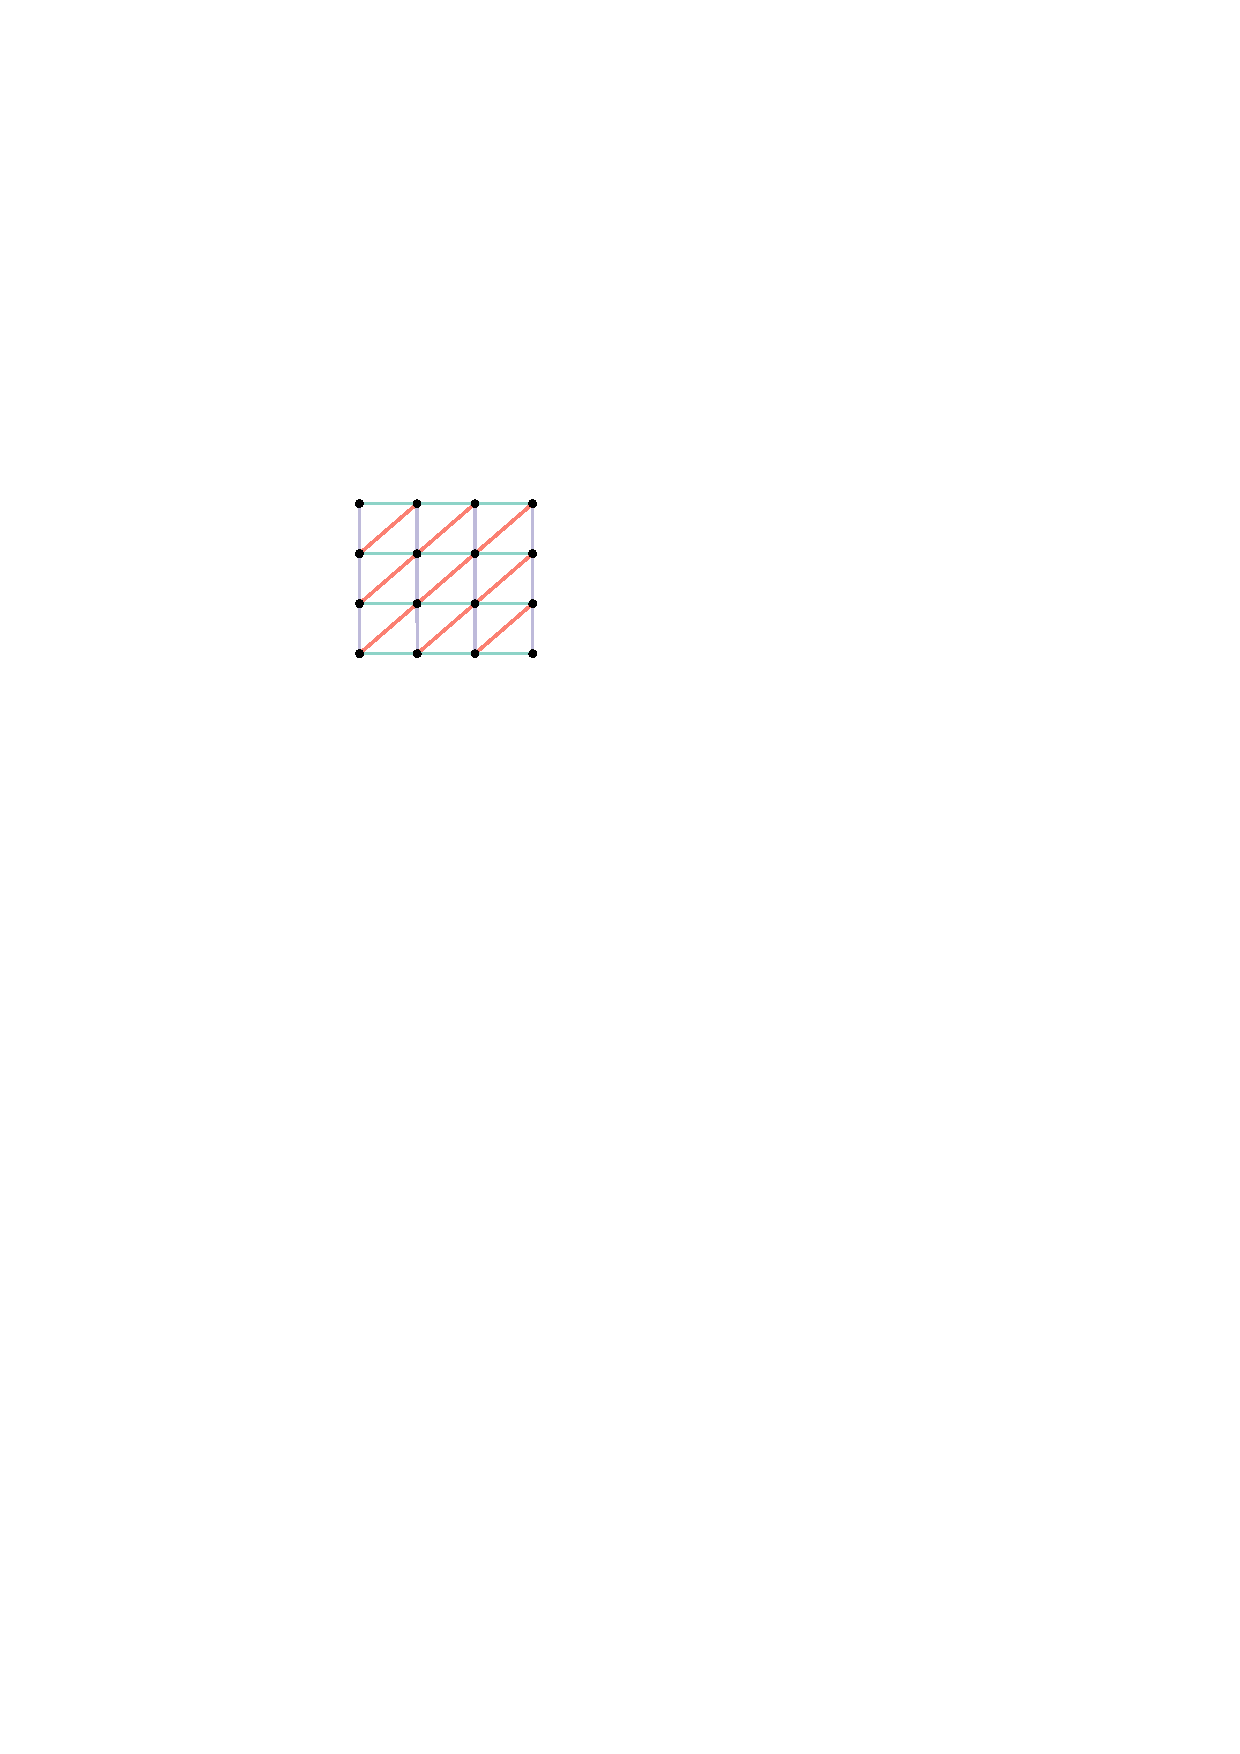
\includegraphics[width=.25\textwidth]{figs/q} & $=$
			& 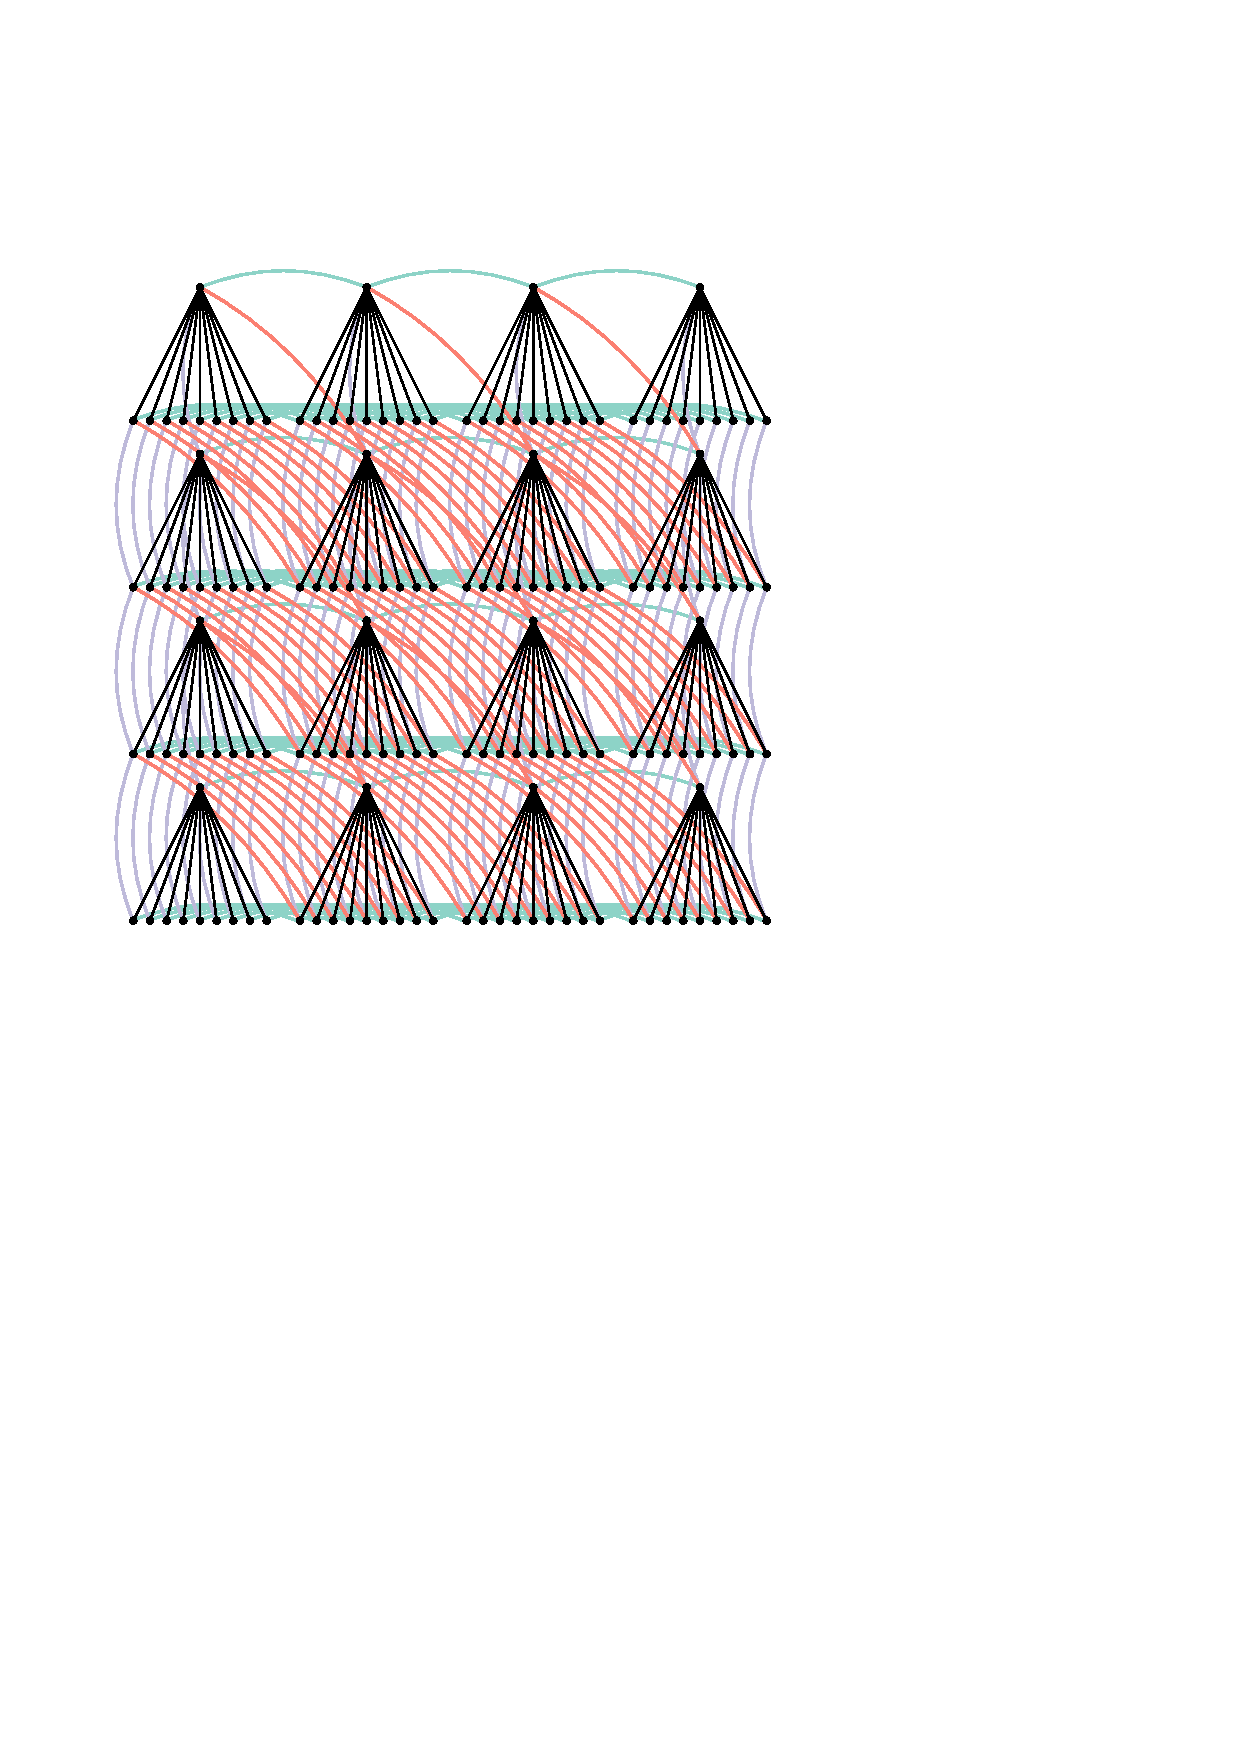
\includegraphics[width=.3\textwidth]{figs/product}
		\end{tabular}
	\end{center}
	% 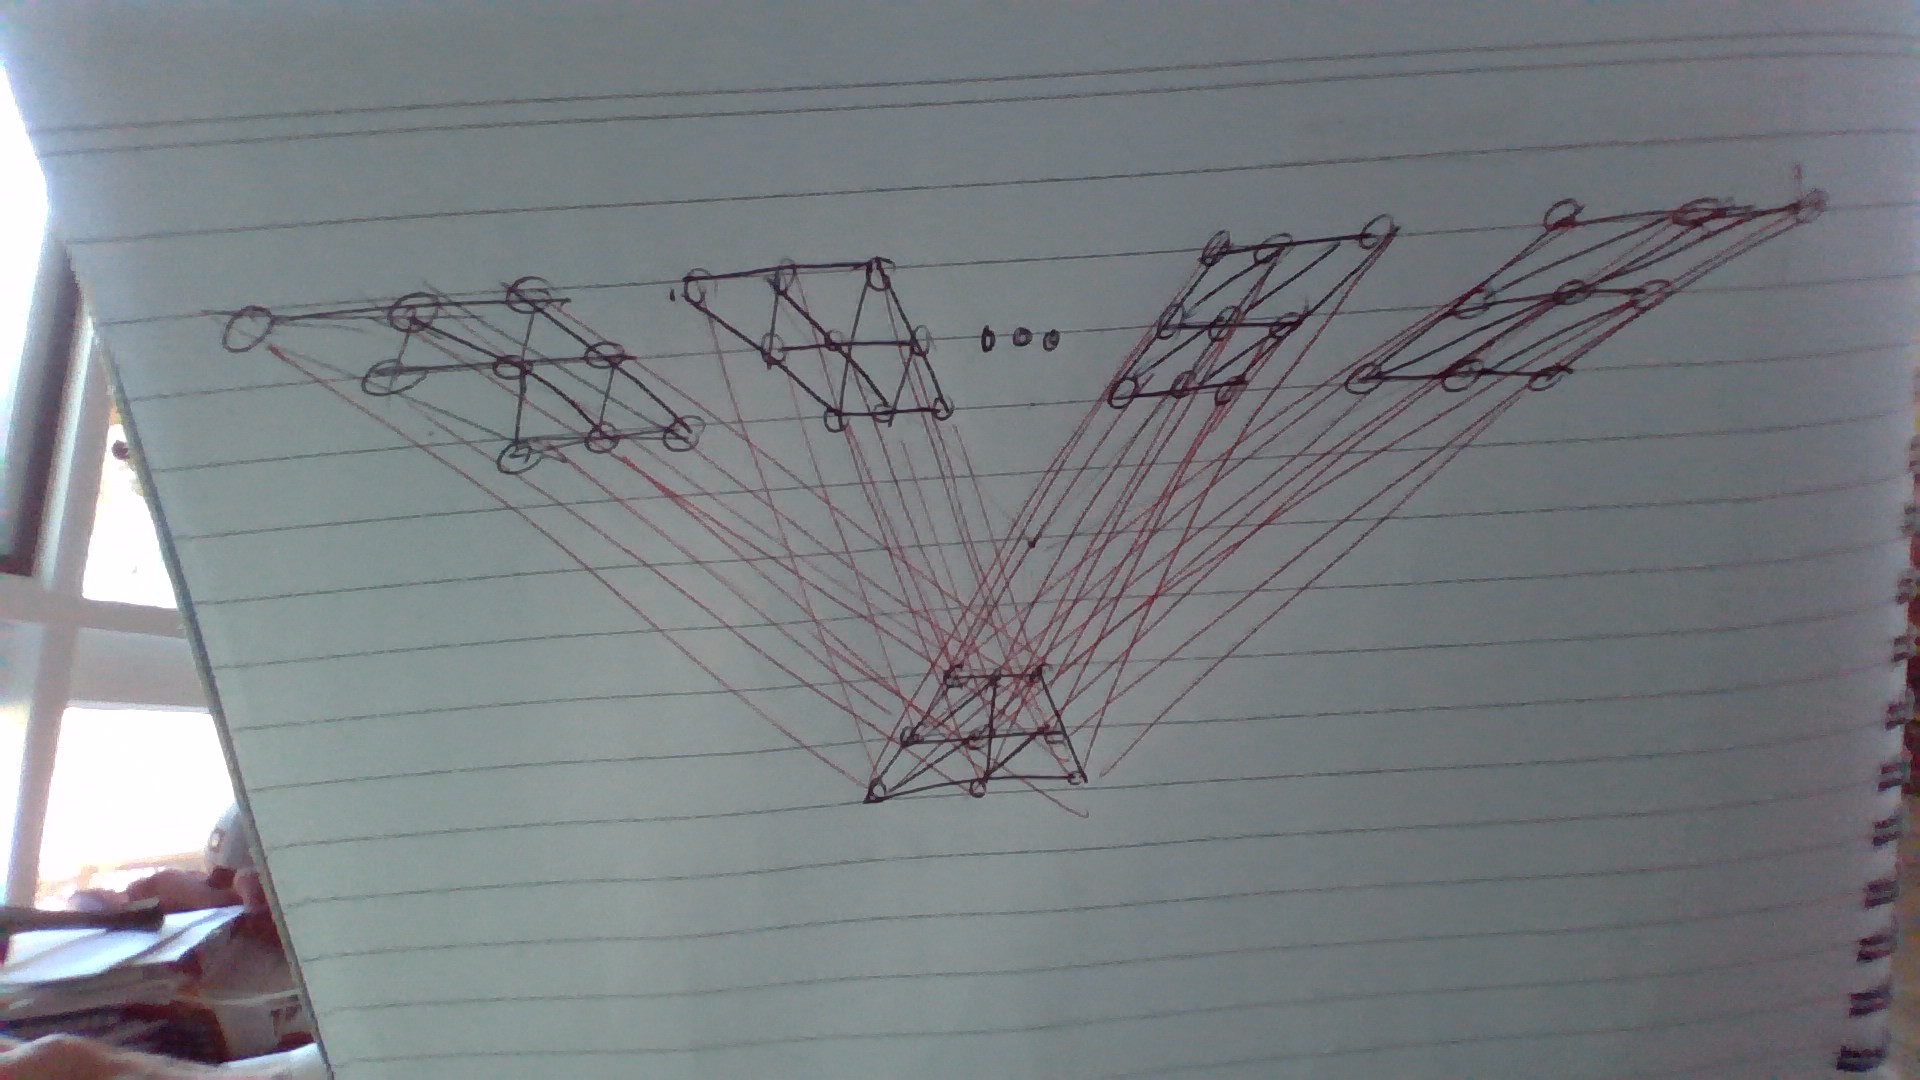
\includegraphics[width=\textwidth]{figs/figure}
	\caption{$S_9 \CartProd H_4$.}
	\label{graph}
\end{figure}


\subsection*{Subdivisions}

A noteworthy consequence of \Cref{family} is that it resolves a conjecture of \citet{BO99}. A graph $G'$ is a \textit{subdivision} of a graph $G$ if $G'$ can be obtained from $G$ by replacing the edges $vw$ of $G$ by internally disjoint paths $P_{vw}$ with endpoints $v$ and $w$. If each $P_{vw}$ has exactly $k$ internal vertices, then $G'$ is the \emph{$k$-subdivision} of $G$. If each $P_{vw}$ has at most $k$ internal vertices, then $G'$ is a \emph{$(\leq k)$-subdivision} of $G$. \citet{BO99} conjectured that the stack-number of $(\leq k)$-subdivisions ($k$ fixed)  is not much less than the stack-number of the original graph. More precisely:

\begin{conj}[\citep{BO99}]
\label{B_conj}
There exists a function $f$ such that for every graph $G$ and integer $k$, if $G'$ is any $(\leq k)$-subdivision of $G$, then $\sn(G) \leq f(\sn(G’),k)$.
\end{conj}

\citet{DujWoo05} established a connection between this conjecture and the question of whether stack-number is bounded by queue-number. In particular, they showed that if
\cref{B_conj} is true, then stack-number is bounded by queue-number. Since \cref{family} shows that stack-number is not bounded by queue-number, \cref{B_conj} is false. The proof of \citet{DujWoo05} is based on the folllowing key lemma: every graph $G$ has a $3$-stack subdivision with $1+2 \ceil{\log_2\qn(G)}$ division vertices per edge. Applying this result to the graph $G=S_b\CartProd H_n$ in \cref{family},
the $5$-subdivision of $S_b\CartProd H_n$ has a $3$-stack layout. If \cref{B_conj} was true, then $\sn(S_b\CartProd H_n) \leq f( 3,5)$, contradicting \cref{family}.

%Specifically,
%\[
%    \mathcal{F} := \{ S_b\square H_n : b,n\in\N\}
%\]
%where $S_b$ denotes the star with $b$ leaves and $H_n$ is the triangulated $n\times n$ grid.

%\todo[inline]{PM: Does anyone know if there is a standard box operator that is typeset like this $S\boxtimes H$ or $S\boxdot H$ instead of like this $S\square H$ or like this $S\Box H$?  I tried square and Box. DW: I defined \texttt{CartProd} which typesets okay $A \CartProd B$	.}


%The graph $G$ in \cref{family} is obtained as follows (See \figref{graph}): Let $S_b$ denote the star graph with root $r$ and $b$ leaves.  For an even positive integer $n$, let $H_n$ be the $n\times n$ triangulated grid, defined by $V(H_n):=\{1,\ldots,n\}^2$ and
%\begin{align*}
%E(H_n) & :=\{(x,y)(x+1,y):x\in\{1,\ldots,n-1\},\,y\in\{1,\ldots,n\}\} \\
%& \qquad \cup \{(x,y)(x,y+1):x\in\{1,\ldots,n\},\,y\in\{1,\ldots,n-1\}\} \\
%& \qquad \cup \{(x,y+1)(x+1,y):x,y\in\{1,\ldots,n-1\}\} \enspace .
%\end{align*}
%We consider the graph $G:=S_b\CartProd H_n$. That is, $V(G)=V(S_b)\times V(H_n)$ where vertices $(v_1,w_1),(v_2,w_2)\in V(G)$ are adjacent whenever $v_1=w_1$ and $v_2w_2\in E(H_n)$, or $v_1w_1\in E(S_b)$ and $v_2=w_2$.


%SAY SOMETHING ABOUT THE RESULTS OF \citet{Pupyrev20}. I EXPECT WE SOLVE SOME OPEN PROBLEM HERE.\todo{PM:Not really, his open problem is about $H\boxtimes P$ where $H$ has bounded treewidth.}

\subsection*{Is Queue-number Bounded by Stack-Number? }

It remains open whether queues are more powerful than stacks; that is, whether queue-number is bounded by stack-number. Several reults are known about this problem. \citet{HLR92} showed that every 1-stack graph has a 2-queue layout. \citet{DJMMUW20} showed that planar graphs have bounded queue-number. (Note that graph products also feature heavily in this proof.)\ Since 2-stack graphs are planar, this implies that 2-stack graphs have bounded queue-number. It is open whether 3-stack graphs have bounded queue-number. In fact, the case of three stacks is as hard as the general question. \citet{DujWoo05} proved that queue-number is bounded by stack-number if and only if 3-stack graphs have bounded queue-number. Moreover, if this is true then stack-number is bounded by a polynomial function of queue-number.


\section{Stack and Queue Layouts of Cartesian Products}

\todo[inline]{Add discussion of result of \citet{BK79}: $\sn(G\CartProd H) \leq \sn(G) + \dsn(H)$ for bipartite $H$. Highlight the key difference between stack and queue layouts is that we need $H$ to be bipartite here.}

\todo{mention results of \citet{Pupyrev20} about bipartite graphs?}

First we prove that $\qn(S_b\CartProd H_n)\leq 4$, as claimed in \cref{family}. We need the following definition due to \citet{Wood-Queue-DMTCS05}. A queue layout $(\varphi,\prec)$ is \emph{strict} if for every vertex $u\in V(G)$ and for all neighbours $v,w\in N_G(u)$, if $u\prec v,w$ or $v,w \prec u$, then $\varphi(uv)\neq \varphi(uw)$. Let $\sqn(G)$ be the minimum integer $k$ such that $G$ has a strict $k$-queue layout. To see that $\sqn(H_n) \leq 3$, order the vertices row-by-row and then left-to-right within a row, with vertical edges in one queue, horizontal edges in one queue, and diagonal edges in another queue.
\citet{Wood-Queue-DMTCS05} proved that $\qn(G \CartProd H) \leq \qn(G) + \sqn(H)$ for all graphs $G$ and $H$. Of course, $S_b$ has a 1-queue layout (since no two edges are nested for any vertex-ordering). Thus $\qn(S_b \CartProd H_n)\leq 4$.

\section{The Main Proof}

We now turn to the proof of our main result, the lower bound on $\sn(G)$, where $G:= S_b\CartProd H_n$. Consider a hypothetical $s$-stack layout $(\varphi,\prec)$ of $G$ where $n$ and $b$ are chosen sufficiently large compared to $s$ as detailed below. We begin with three lemmata that, for sufficiently large $b$, provide a large subgraph $S_d$ of $S_b$ for which the induced stack layout of $S_d\CartProd H_n$ is highly structured.

For each node $v$ of $S_b$, define $\pi_v$ as the permutation of $\{1,\ldots,n\}^2$ in which $(x_1,y_1)$ appears before $(x_2,y_2)$ if and only if $(v,(x_1,y_1))\prec (v,(x_2,y_2))$. The following lemma is an immediate consequence of the Pigeonhole Principle:

\begin{lem}\lemlabel{uniform_order}
    There exists a permutation $\pi$ of $\{1,\ldots,n\}^2$ and a set $L_1$ of leaves of $S_b$ of size $a\ge b/(n^2)!$ such that $\pi_{v}=\pi$ for each $v\in L_1$.
\end{lem}

% \todo[inline]{If we cared, we could improve this to $b/2^{cn^2}$ since we only use the weaker property (P3) in the final proof. DW: I don't care. }

For each leaf $v$ in $L_1$, let $\varphi_v$ be the edge colouring of $H_n$ defined by $\varphi_v(x,y):=\varphi(v,(x,y))$. Since $H_n$ has maximum degree $6$ and is not 6-regular, it has fewer than $3n^2$ edges.  Therefore there are fewer than $s^{3n^2}$ edge colourings of $H_n$ using $s$ colours.  Another application of the Pigeonhole Principle proves the following:

\begin{lem}\lemlabel{uniform_colour}
    There exists a subset $L_2\subseteq L_1$ of size $c\ge a/s^{3n^2}$
    and an edge colouring $\phi:E(H_n)\to\{1,\ldots,s\}$ such that $\varphi_v=\phi$ for each $v\in L_2$.
\end{lem}


Let $S_{c}$ be the subgraph of $S_b$ induced by $L_2\cup\{r\}$. The preceding two lemmata ensure that, for distinct leaves $v$ and $w$ of $S_{c}$, the stack layouts of the isomorphic graphs $G[\{(v,p):p\in V(H_n)\}]$ and $G[\{(w,p):p\in V(H_n)\}]$ are identical. The next lemma is a statement about the relationships between the stack layouts of $G[\{(v,p):v\in V(S_{c})\}]$ and $G[\{(v,q):v\in V(S_{c})\}]$ for  distinct $p,q\in V(H_n)$.  It does not assert that these two layouts are identical but it does state that they fall into one of two categories.

\begin{lem}\lemlabel{forward_or_backward}
    There exists a sequence $L_3:=u_1,\ldots,u_{d}$ with $\{u_1,\ldots,u_{d}\}\subseteq L_2$ of length $d\ge c^{1/2^{n^2-1}}$ such that, for each $p\in V(H_n)$, either  $(u_1,p)\prec (u_2,p)\prec\cdots\prec (u_{d},p)$ or $(u_1,p)\succ (u_2,p)\succ\cdots\succ (u_{d},p)$.
\end{lem}

\begin{proof}
    Let $p_1,\ldots,p_{n^2}$ denote the vertices of $H_n$ in any order.
    Begin with the sequence $S_1:=v_{1,1},\ldots,v_{1,c}$ that contains all $c$ elements of $L_2$ ordered so that $(v_{1,1},p_1)\prec\cdots\prec(v_{1,c},p_1)$.  For each $i\in\{2,\ldots,n^2\}$, the Erd\H{o}s-Szekeres Theorem~\citep{ES35} implies that $S_{i-1}$ contains a subsequence $S_i:=v_{i,1},\ldots,v_{i,|S_i|}$ of length $|S_i|\ge \sqrt{|S_{i-1}|}$ such that $(v_{i,1},p_i)\prec\cdots\prec(v_{i,d_i},p_i)$ or $(v_{i,1},p_i)\succ\cdots\succ(v_{i,d_i},p_i)$.  It is straightforward to verify by induction on $i$ that $d_i \ge c^{1/2^{i-1}}$ resulting in a final sequence $S_{n^2}=:L_3$ of length at least $c^{1/2^{n^2-1}}$.
\end{proof}

For the rest of the proof we will work with the star $S_d$ whose leaves are $u_1,\ldots,u_d$ described in \lemref{forward_or_backward}.  Consider the (improper) vertex colouring of $H_n$ obtained by colouring each vertex $p\in V(H_n)$ \emph{red} if $(u_1,p)\prec\cdots\prec (u_d,p)$ and colouring $p$ \emph{blue} if $(u_1,p)\succ\cdots\succ(u_d,p)$. We need the following famous Hex Lemma~\citep{Gale79}.

\begin{lem}[\citep{Gale79}] \label{hex_lemma}
Every red--blue vertex colouring of the graph $H_n$	contains an $n$-vertex path $R$ consisting entirely of red vertices or entirely of blue vertices.
\end{lem}

%\begin{proof}
%    The dual of $H_n$ is the board on which the game Hex is played.  The well-known \emph{Hex Lemma} states that any colouring of the vertices of $H_n$ with colours red and blue contains exactly one of the following \cite{Gale79}:
%    \begin{compactenum}
%        \item a path with endpoints $(x,1)$ and $(x',n)$ consisting entirely of red vertices, for some $x,x'\in\{1,\ldots,n\}$; or
%        \item a path with endpoints $(1,y)$ and $(n,y')$ consisting entirely of blue vertices, for some $y,y'\in\{1,\ldots,n\}$.
%    \end{compactenum}
%    In either case, the path contains at least $n$ vertices and therefore has a $n$-vertex subpath consisting entirely of red vertices or entirely of blue vertices.
%\end{proof}

Without loss of generality, assume that the path $R:=p_1,\ldots,p_n$ defined by \cref{hex_lemma} (with the above-defined colouring) consists entirely of red vertices, so that $(u_1,p_j)\prec\cdots\prec (u_d,p_j)$ for each $j\in\{1,\ldots,n\}$.  Recall that $(\varphi,\prec)$ is a hypothetical $s$-stack layout of $G$ and therefore it is also an $s$-stack layout of the subgraph $X:=S_d\CartProd R$. In particular, there is no set of greater than $s$ pairwise crossing edges in $X$. The following result finishes the proof by showing that such a set exists when $n> 2s$ and $d\ge (s+1)2^{n}$ (which is implied if $n=2s+1$ and $b \ge (n^2)!\, s^{3n^2}\, ((s+1)2^n)^{2^{n^2-1}} $).


\begin{lem}\lemlabel{twister}
    The graph $X$ contains a set of edges of size at least $\min\{\lfloor d/2^{n}\rfloor,\lceil n/2\rceil\}$ that are pairwise crossing with respect to $\prec$.
\end{lem}

\begin{proof}
    We will define sets $A_1\supseteq \cdots\supseteq A_{n}$ of leaves of $S_d$ so that each $A_i$ satisifies the following conditions:
    \begin{compactenum}[(C1)]
        \item $A_i$ contains $d_i\ge d/2^{i-1}$ leaves of $S_d$.
        \item Each leaf $v\in A_i$ defines an $i$-element vertex set $Z_{i,v}:=\{(v,p_j):j\in\{1,\ldots,i\}\}$.  For any distinct $v,w\in A_i$, the sets $Z_{i,v}$ and $Z_{i,w}$ are \emph{separated} with respect to $\prec$; that is, $Z_{i,v}\prec Z_{i,w}$ or $Z_{i,v}\succ Z_{i,w}$.
    \end{compactenum}

    Before defining $A_1,\ldots,A_n$ we first show how the existence of the set $A_n$ implies the lemma.  To avoid triple-subscripts, let $d':=d_n\ge d/2^{n-1}$.   The set $A_n$ defines vertex sets $Z_{n,v_1}\prec\cdots\prec Z_{n,v_{d'}}$.  Refer to \figref{twister}. Recall that $r$ is the root of $S_b$ so it is adjacent to each of $v_{1},\ldots,v_{d'}$ in $S_d$.  Therefore, for each $j\in\{1,\ldots,n\}$ and each $i\in\{1,\ldots,d'\}$, the edge $(r,p_j)(v_i,p_j)$ is in $X$. Therefore, $(r,p_j)$ is adjacent to an element of each of $Z_{n,v_1},\ldots,Z_{n,v_{d'}}$.
	\begin{figure}
		\begin{center}
			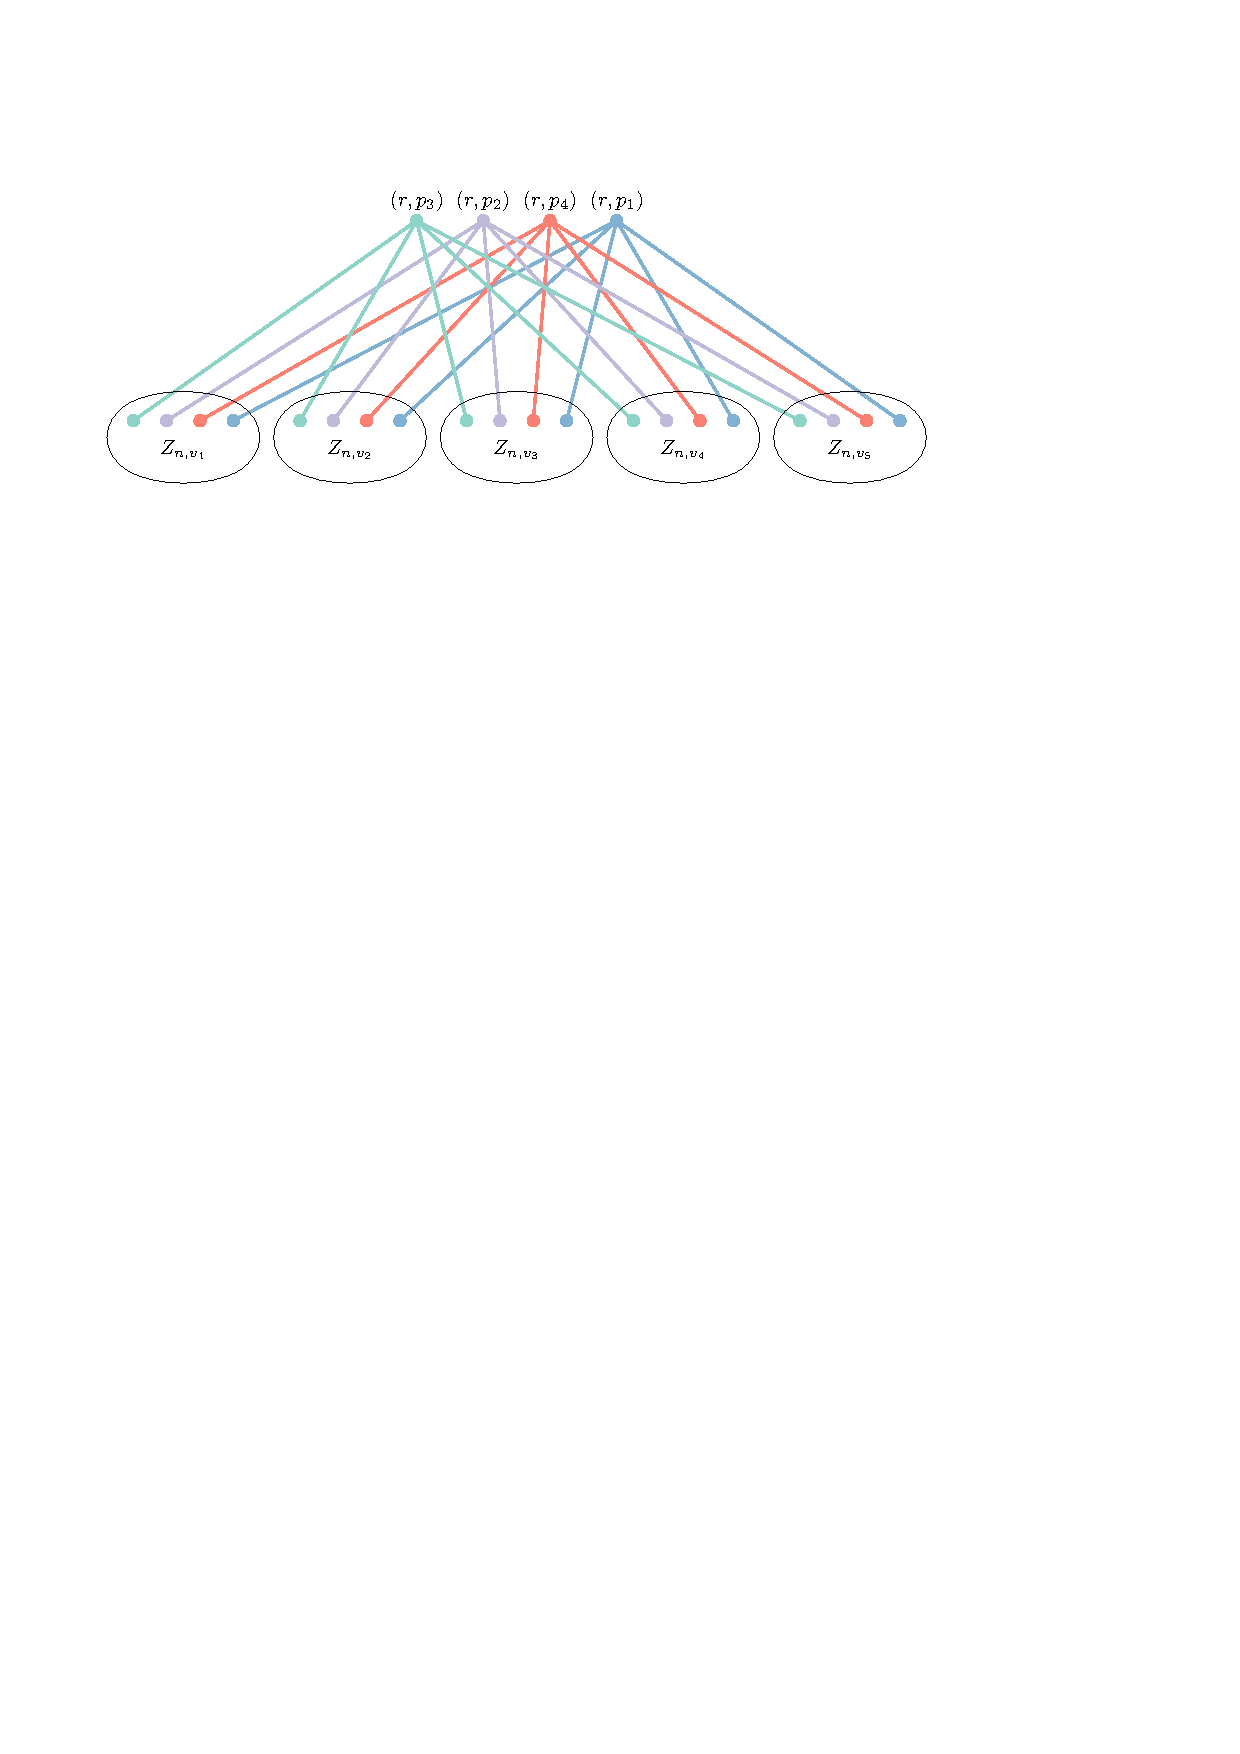
\includegraphics{figs/twister}
		\end{center}
		\caption{The sets $Z_{n,v_1},\ldots,Z_{n,v_{d'}}$ ($n=4$, $d'=5$).}
		\figlabel{twister}
	\end{figure}

    Since $Z_{n,v_1},\ldots,Z_{n,v_{d'}}$ are separated with respect to $\prec$, when viewed from afar, this situation looks like a complete bipartite graph $K_{n,d'}$ with the root vertices $L:=\{(r,p_j):j\in\{1,\ldots,n\}\}$ in one part and the groups $R:=Z_{n,v_1}\cup\cdots\cup Z_{n,v_{d'}}$ in the other part.  Any linear ordering of $K_{n,d'}$ has a large set of pairwise crossing edges so, intuitively, the induced subgraph $X[L\cup R]$ should also have a large set of pairwise crossing edges. We can formalize this as follows: Label the vertices in $L$ as $r_1,\ldots,r_n$ so that $r_1\prec \cdots\prec r_{n}$.  Then at least one of the following two cases applies (see \figref{median}):
    \begin{enumerate}
        \item $Z_{n,\lfloor d'/2\rfloor}\prec r_{\lceil n/2\rceil}$ in which case the graph between $r_{\lceil n/2\rceil},\ldots,r_{n}$ and $Z_{n,1},\ldots,Z_{n,\lfloor d'/2\rfloor}$ has a set of at least $\min\{\lfloor d'/2\rfloor,\lceil n/2\rceil\}$ pairwise-crossing edges.
        \item $r_{\lceil n/2\rceil}\prec Z_{\lceil d'/2\rceil+1}$ in which case the graph between $r_1,\ldots,r_{\lceil n/2\rceil}$ and $Z_{\lceil d'/2\rceil+1},\ldots,Z_{d'}$ has a set of $\min\{\lfloor d'/2\rfloor,\lceil n/2\rceil\}$ pairwise-crossing edges.
    \end{enumerate}
	\begin{figure}
		\begin{center}
			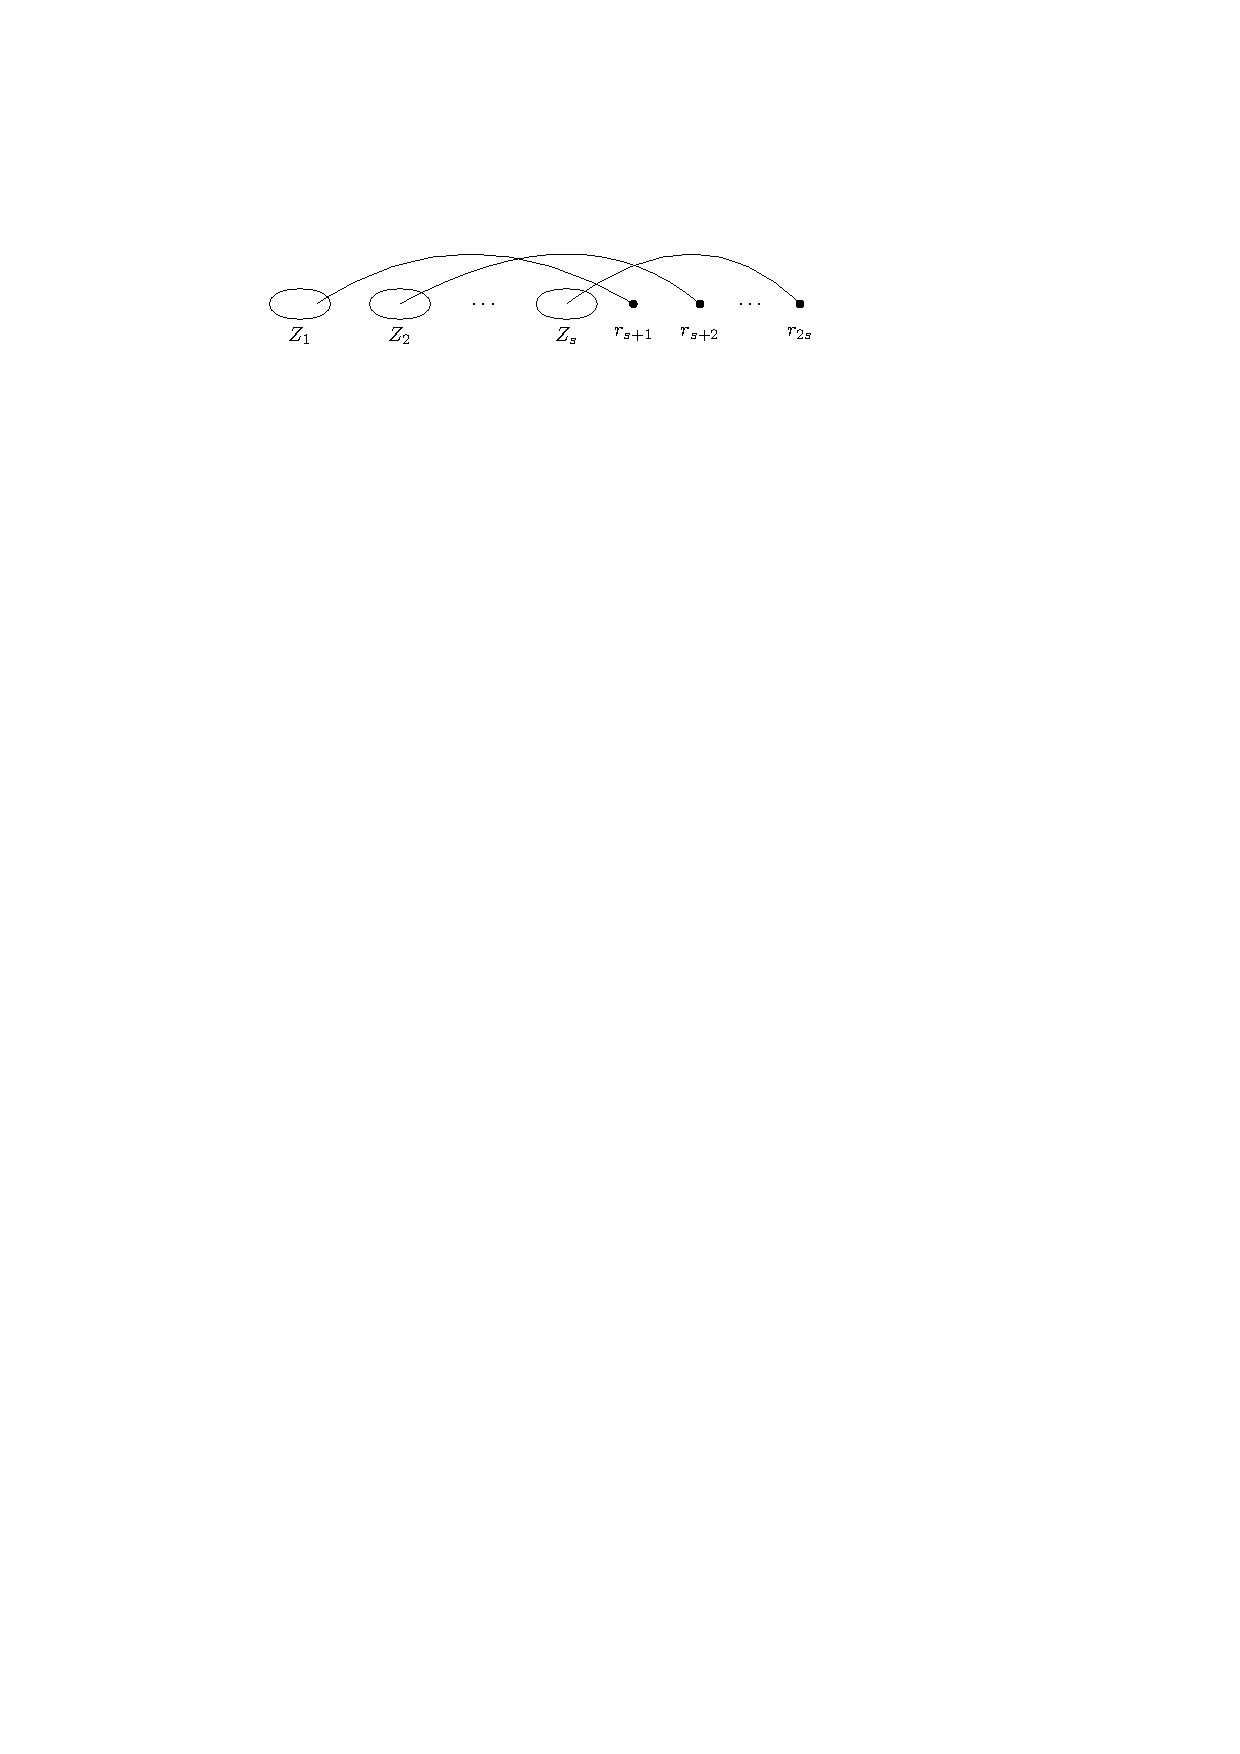
\includegraphics{figs/median-1} \\ 1 \\[2em]
			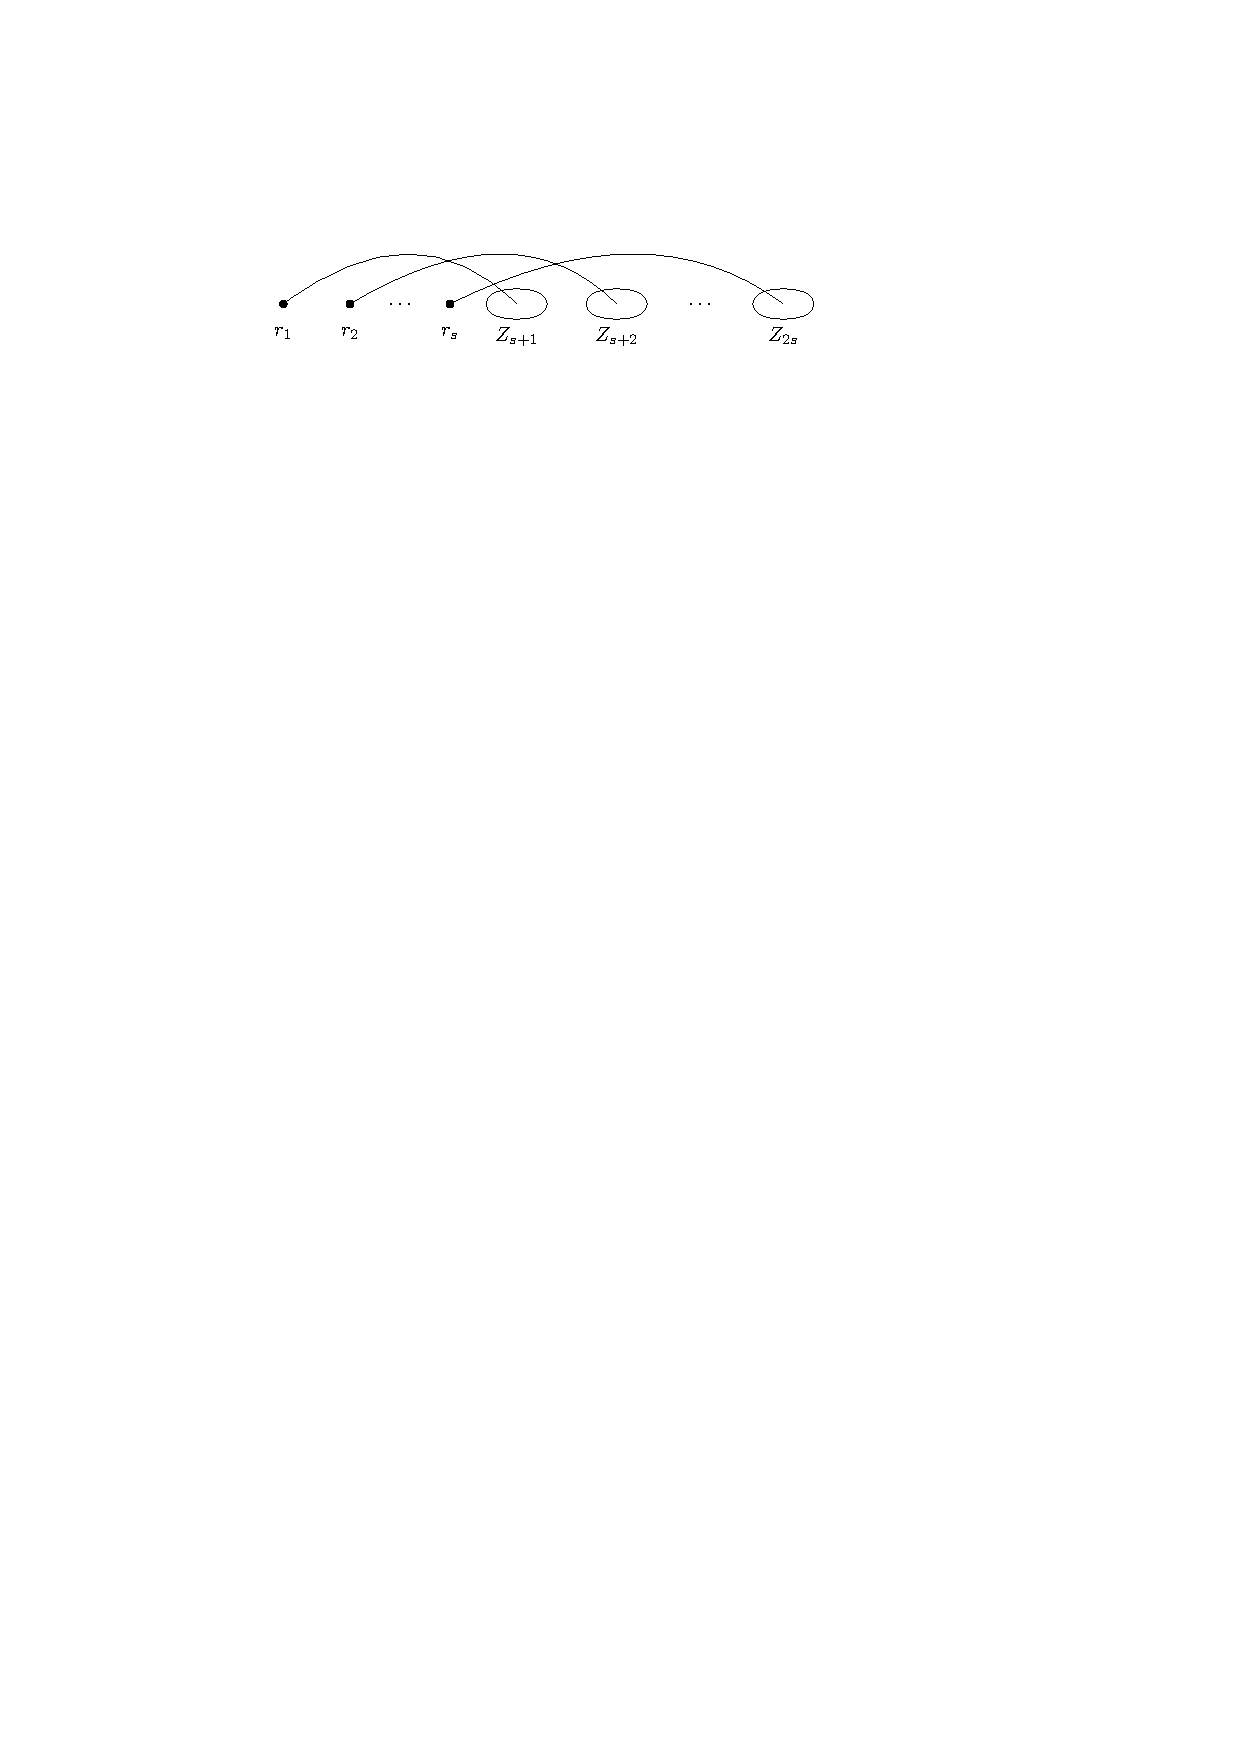
\includegraphics{figs/median-2} \\ 2
		\end{center}
		\caption{The two cases in the proof of \lemref{twister}.}
		\figlabel{median}
	\end{figure}
	Since, by (C1), $d'\ge d/2^{n-1}$, either case results in a set of pairwise-crossing edges of size at least $\min\{\lfloor d/2^n\rfloor,\lceil n/2\rceil\}$, as claimed.

    All that remains is to define the sets $A_1\supseteq\cdots\supseteq A_n$ that satisfy (C1) and (C2).  Let $A_1$ be the set of all the leaves of $S_d$.  For each $i\in\{2,\ldots,n\}$, the set $A_i$ is defined as follows:  Let $Z_1,\ldots,Z_{|A_{i-1}}$ denote the sets $Z_{i-1, v}$ for each $v\in A_{i-1}$ ordered so that $Z_1\prec\cdots\prec Z_r$. By Property (C2), this is always possible.	Label the vertices of $A_{i-1}$ as $v_1,\ldots,v_{|A_{i-1}|}$ so that $(v_1,p_{i-1})\prec\cdots\prec (v_r,p_{i-1})$.   (This is equivalent to naming them so that $(v_j,p_{i-1})\in Z_j$ for each $j\in\{1,\ldots,|A_{i-1}|\}$.)  Define the set $A_i:=\{v_{2k+1}:k\in\{0,\ldots,\lfloor(|A_{i-1}|-1)/2\rfloor\}\}=\{v_{j}\in A_{i-1}:\text{$j$ is odd}\}$.  This completes the definition of $A_1,\ldots,A_n$.

	All that remains is to verify that $A_i$ satisfies (C1) and (C2).  We do this by induction on $i$. The base case $i=1$ is trivial so we assume from this point on that $i\in\{2,\ldots,n\}$.   To see that $A_i$ satisfies (C1) just observe that $|A_i|=\lceil |A_{i-1}|/2\rceil \ge |A_{i-1}|/2\ge d/2^{i-1}$, where the final inequality follows by applying the inductive hypothesis $|A_{i-1}|\ge d/2^{i-2}$.  All that remains is to show that $A_i$ satisfies (C2).

    For each $j\in\{i-1,i\}$, let $H^j:=\{(v,p_j):v\in A_{i-1}\}$.     Recall that, for each $v\in A_{i-1}$, the edge $e_v:=(v,p_{i-1})(v,p_i)$ is in $X$.  We have the following properties:
    \begin{compactenum}[(P1)]
        \item By \lemref{uniform_colour}, $\varphi(e_v)=\phi(p_{i-1}p_i)$ for each $v\in A_{i-1}$.
        \item Since $p_{i-1}$ and $p_i$ are both red, $(v,p_{i-1})\prec (w,p_{i-1})$ if and only if $(v,p_{i})\prec (w,p_{i})$ for each $v,w\in A_{i-1}$.
        \item By \lemref{uniform_order}, $(v,p_{i-1})\prec (v,p_i)$ for every $v\in A_{i-1}$ or $(v,p_{i-1})\succ (v,p_i)$ for every $v\in A_{i-1}$.
    \end{compactenum}
    We claim that these three conditions imply that the vertex sets of $H^{i-1}$ and $H^{i}$ interleave perfectly with respect to $\prec$. More precisely:
	\begin{clm}\clmlabel{interleave} $(v_1,p_{i-1+t})\prec (v_1,p_{i-t}) \prec (v_2,p_{i-1+t}) \prec (v_2,p_{i-t}) \cdots \prec (v_r,p_{i-1+t}) \prec (v_r,p_{i-t})$ for some $t\in\{0,1\}$.
	\end{clm}
	\begin{proof}[Proof of \clmref{interleave}]
		By (P3) we may assume, without loss of generality, that $(v,p_{i-1})\prec (v,p_i)$ for each $v\in A_{i-1}$, in which case we are trying to prove the claim for $t=0$.  Therefore, it is sufficient to show that $(v_j,p_i)\prec (v_{j+1},p_{i-1})$ for each $j\in\{1,\ldots,r-1\}$.  For the sake of contradiction, suppose $(v_j,p_{i})\succ (v_{j+1},p_{i-1})$ for some $j\in\{1,\ldots,r-1\}$. By the labelling of $A_{i-1}$,  $(v_j,p_{i-1})\prec (v_{j+1},p_{i-1})$ so, by (P2),  $(v_{j},p_i) \prec (v_{j+1},p_i)$.  Therefore
		\[
			(v_j,p_{i-1})\prec (v_{j+1},p_{i-1})\prec(v_{j},p_i) \prec
		   (v_{j+1}, p_i) \enspace .
	   	\]
		Therefore the edges $e_{v_j}=(v_j,p_{i-1})(v_j,p_{i})$ and $e_{v_{j+1}}=(v_{j+1},p_{i-1})(v_{j+1},p_i)$ cross with respect to $\prec$.  But this is a contradiction since, by (P1),  $\varphi(e_{v_j}) =\varphi(e_{v_{j+1}})=\phi(p_{i-1}p_i)$.
		This contradiction completes the proof of \clmref{interleave}.
	\end{proof}

% \todo{DW: Why are these $\prec$'s red?  PM: Just me keeping track of which one was the assumption, they don't need to be red.}

We now complete the proof that $A_i$ satisfies (C2). Apply \clmref{interleave} and assume without loss of generality that $t=0$, so that
	\[
		(v_1,p_{i-1})\prec (v_1,p_{i}) \prec (v_2,p_{i-1}) \prec (v_2,p_{i}) \cdots \prec (v_r,p_{i-1}) \prec (v_r,p_{i}) \enspace .
	\]

    For each $j\in\{1,\ldots,r-2\}$, we have $(v_{j+1},p_{i-1})\in Z_{j+1}\prec Z_{j+2}$, so  $(v_j,p_i)\prec (v_{j+1},p_{i-1}) \prec Z_{j+2}$.  Therefore $Z_j\cup\{(v_j,p_i)\} \prec Z_{j+2}$.  By a symmetric argument, $Z_j\cup\{(v_j,p_i)\} \succ Z_{j-2}$ for each  $j\in\{3,\ldots,r\}$.  Finally, since $(v_{j},p_i)\prec (v_{j+2},p_i)$ for each odd $i\in\{1,\ldots,r\}$, we have $Z_{j}\cup\{(v_j,p_i)\} \prec Z_{j+2}\cup\{(v_{j+2},p_i)\}$ for each odd $j\in\{1,\ldots,r-2\}$.  Thus $A_i$ satisifies (C2) since the sets $Z_1\cup\{(v_1,p_i)\},Z_3\cup\{(v_3,p_i)\},\ldots,Z_{2\lfloor (r-1)/2\rfloor+1} \cup (v_{2\lfloor (r-1)/2\rfloor+1},p_i)$ are precisely the sets $Z_{i,1},\ldots,Z_{i,d_i}$ determined by our choice of $A_i$.
\end{proof}

% \begin{lem}\lemlabel{twister}
%     Let $G$ be any graph, let $\prec$ be any linear ordering of $V(G)$,  let $Z_{1}\prec\cdots\prec Z_{2s}$ be subsets of $V(G)$, and let $r_1\prec\cdots\prec r_{2s}$ be vertices of $G$ such that, for each $i,j\in\{1,\ldots,2s\}$, $G$ contains an edge $r_iz_j$ with $z_j\in Z_j$. Then $G$ contains a set of $s$ edges that are pairwise crossing with respect to $\prec$. \todo[inline]{I think we should not re-use $s$ in this lemma. More importantly, do we really need Lemma 6? It could be easily merged into the proof of Lemma 5 where Lemma 6 is used, and this would avoid having to translate notation. It took me a while to realise that $r_1,\dots,r_{2s}$ corresponds to $L$ in Lemma 5.}
% \end{lem}
%
% \begin{proof}
% \end{proof}
%
\section{Open Problems}

Recall that every 1-queue graph has a 2-stack layout \citep{HLR92} and we proved that there are 4-queue graphs with unbounded stack-number. The following questions remain open: Do 2-queue graphs have bounded stack-number? Do 3-queue graphs have bounded stack-number?

Given the role of cartesian products in our proof, it is natural to ask when is $\sn(G_1\CartProd G_2)$ bounded? Note that $H_n$ is a subgraph of a planar Hamiltonian graphs (namely, $H_{2n}$), so $\sn(H_n) \leq 2$. So $\sn(G_1\CartProd G_2)$ can be unbounded even when $G_1$ is a star and $\sn(G_2)\leq 2$.
Since $\sn(G_2)\leq 1$ if and only if $G_2$ is outerplanar, the following question naturally arises: Is $\sn(S \CartProd H)$ bounded for every star $S$ and outerplanar graph $H$ with bounded degree? Is $\sn(T \CartProd H)$ bounded for every tree $T$ and outerplanar graph $H$ with bounded degree? The assumption that $H$ has bounded degree is needed since $S_n \CartProd S_n$ contain the 1-subdivision of $K_{n,n}$, which has unbounded stack-number~\citep{Blankenship-PhD03}.

Since $H_n\subseteq P \boxtimes P$ where $P$ is the $n$-vertex path, \cref{family} implies that $\sn(S\boxtimes P\boxtimes P)$ is unbounded for stars $S$ and paths $P$. It is easily seen that $\sn(S\boxtimes P)$ is bounded~\citep{Pupyrev20}. The following question naturally arises (independently asked by \citet{Pupyrev20}):
Is $\sn(T \boxtimes P)$ bounded for every tree $T$ and path $P$? We conjecture the answer is ``no''.

\let\oldthebibliography=\thebibliography
\let\endoldthebibliography=\endthebibliography
\renewenvironment{thebibliography}[1]{%
\begin{oldthebibliography}{#1}%
\setlength{\parskip}{0ex}%
\setlength{\itemsep}{0ex}%
}{\end{oldthebibliography}}

%\documentclass[kpfonts]{patmorin}
\usepackage{pat}
\usepackage{paralist,graphicx}
\usepackage{array,longtable}

\usepackage[utf8]{inputenc}
\usepackage{todonotes}

\usepackage[noabbrev,capitalise]{cleveref}
\crefname{lem}{Lemma}{Lemmas}
\crefname{thm}{Theorem}{Theorems}
\crefname{cor}{Corollary}{Corollaries}
\crefname{prop}{Proposition}{Propositions}
\crefname{conj}{Conjecture}{Conjectures}
\crefname{open}{Open Problem}{Open Problems}
\crefname{obs}{Observation}{Observations}

\crefformat{equation}{(#2#1#3)}
\Crefformat{equation}{Equation #2(#1)#3}

\usepackage[numbers,sort&compress]{natbib}
\usepackage{hypernat}
\makeatletter
\def\NAT@spacechar{~}
\makeatother

\setlength{\parskip}{1ex}
\setlength{\parindent}{0ex}

\newtheorem{property}{Property}
\newcommand{\plabel}[1]{\label{prop:#1}}
\newcommand{\pref}[1]{Property~\ref{prop:#1}}

\DeclareMathOperator{\sn}{sn}
\DeclareMathOperator{\qn}{qn}
\DeclareMathOperator{\sqn}{sqn}
\DeclareMathOperator{\dsn}{dsn}
\DeclareMathOperator{\tw}{tw}

\renewcommand{\SS}{\mathcal{S}}

\renewcommand{\le}{\leqslant}
\renewcommand{\leq}{\leqslant}
\renewcommand{\ge}{\geqslant}
\renewcommand{\geq}{\geqslant}

\newcommand{\CartProd}{\mathbin{\square}}

\title{\MakeUppercase{Stack-Number is not Bounded by Queue-Number}}

\author{%
	Vida Dujmovi\'c,\!\!%
	\thanks{School of Computer Science and Electrical Engineering,
		University of Ottawa, Ottawa, Canada (\texttt{vida.dujmovic@uottawa.ca}).
		Research supported by NSERC.}
	\,\,
	Robert Hickingbotham,\!\!%
	\thanks{School of Mathematics, Monash University, Melbourne, Australia (\texttt{robert.hickingbotham@monash.edu}).}
	\,\,
	Pat Morin,\!\!%
	\thanks{School of Computer Science, Carleton University, Ottawa, Canada (\texttt{morin@scs.carleton.ca}). Research  supported by NSERC.}
	\,\,
	David R. Wood\thanks{School of Mathematics, Monash University, Melbourne, Australia (\texttt{david.wood@monash.edu}). Research supported by the Australian Research Council.}
}

\author{TBD}

\begin{document}
\maketitle

\begin{abstract}
We describe a family of graphs with queue-number at most 4 but unbounded stack-number. This resolves open problems of Heath, Leighton and Rosenberg (1992) and Blankenship and Oporwoski (1999).
\end{abstract}

\bigskip

\section{Introduction}

Stacks and queues are fundamental data structures in computer science, but which is more powerful? In 1992, Heath, Leighton and Rosenberg~\cite{HLR92,HR92} introduced an approach for answering this question by defining the graph parameters \textit{stack-number} and \textit{queue-number} (defined below), which respectively measure the power of stacks and queues for representing graphs. The following fundamental problems, implicit in \citep{HLR92,HR92}, were made explicit by \citet{DujWoo05}\footnote{A \emph{graph parameter} is a function $\alpha$ such that $\alpha(G)\in\mathbb{R}$ for every graph $G$ and such that $\alpha(G_1)=\alpha(G_2)$ for all isomorphic graphs $G_1$ and $G_2$. A graph parameter $\alpha$ is \textit{bounded} by a graph parameter $\beta$ if there exists a function $f$ such that $\alpha(G) \leq f(\beta(G))$ for every graph $G$.}:
\begin{compactitem}
	\item Is stack-number bounded by queue-number?
	\item Is queue-number bounded by stack-number?
\end{compactitem}

If stack-number is bounded by queue-number but queue-number is not bounded by stack-number, then stacks would be considered to be more powerful than queues. Similarly, if the converse holds, then queues would be considered to be more powerful than stacks. Despite extensive research on stack- and queue-numbers, these fundamental questions have remained unsolved.

We now formally define stack- and queue-number.
Let $G$ be a graph and let $\prec$ be a total order on $V(G)$.  Two disjoint edges $vw,xy\in E(G)$ with $v\prec w$ and $x\prec y$ \emph{cross} with respect to $\prec$ if $v\prec x\prec w\prec y$ or $x\prec v\prec y\prec w$, and \emph{nest} with respect to $\prec$ if $v\prec x\prec y\prec w$ or $x\prec v\prec w\prec y$.
%A set of $k$ pairwise nested edges is called a \emph{$k$-rainbow} and a set of $k$ pairwise crossing edges is called a \emph{$k$-twist}. A set of $k$ edges, no pair of which nest and no pair of which cross is called a \emph{hopper}.
Let $\varphi:E(G)\to\{1,\ldots,k\}$ for some integer $k\ge 1$.  Then $(\prec,\varphi)$ is a \emph{$k$-stack layout} of $G$ if, for every pair of edges $vw,xy\in E(G)$, if $\varphi(vw) = \varphi(xy)$ then $vw$ and $xy$ do not cross.\todo{PM: Suggestion: Replace second if then with $\varphi(vw)\neq\varphi(xy)$ or $vw$ and $xy$ do not cross.} Similarly, the pair $(\prec,\varphi)$ is a \emph{$k$-queue layout} of $G$ if, for every pair of edges $vw,xy\in E(G)$, if $\varphi(vw)=\varphi(xy)$ then  $vw$ and $xy$ do not nest. The smallest integer $s$ for which $G$ has an $s$-stack layout is called the \emph{stack-number} of $G$, denoted  $\sn(G)$. The smallest integer $q$ for which $G$ has a $q$-queue layout is called the \emph{queue-number} of $G$, denoted $\qn(G)$. Note that stack layouts are equivalent to book embeddings (first defined by \citet{Ollmann73}), and stack-number is also known as \emph{page-number}, \emph{book-thickness} or \emph{fixed outer-thickness}. See \citep{BK79,DujWoo04,DujWoo-DCG07,DJMMUW20,DFP13,BFGMMRU19,Yannakakis89,Yann20,MBKPRU20} and the references therein for work on stack- and queue-layouts.

Given a $k$-stack layout $(\prec,\varphi)$ of a graph $G$, for each $i\in\{1,\dots,k\}$, the set $\varphi^{-1}(i)$ behaves like a stack, in the sense that each edge $vw \in \varphi^{-1}(i)$ with $v\prec w$ corresponds to an element in a sequence of stack operations, such that if we traverse the vertices in the order of $\prec$, then $vw$ is pushed onto the stack at $v$ and popped off the stack at $w$. Similarly, each set $\varphi^{-1}(i)$ in a queue layout  behaves like a queue. In this way, the stack-number and queue-number  respectively measure the power of stacks and queues to represent graphs.


\subsection*{Is Stack-Number Bounded by Queue-number?}

This paper considers the first of the above questions. In a positive direction, \citet{HLR92}  showed that every 1-queue graph has a $2$-stack layout. On the other hand, they described graphs that need exponentially more stacks than queues. In particular, $n$-vertex ternary hypercubes have queue-number $O(\log n)$ and stack-number $\Omega(n^{1/9-\epsilon})$ for any $\epsilon>0$.

%Note that, in an $s$-stack layout, $(\prec,\varphi)$, $\varphi$ is a proper $s$-colouring of the auxilliary graph $H$ with vertex set $V(H)=E(G)$ and in which the edge $ef$ if present if and only if $e$ and $f$ cross with respect to $\varphi$.  Any $k$-twist in $G$ with respect to $\prec$ corresponds to a $k$-clique $H$.  Since the chromatic number of any graph is bounded by its clique number, the following observation is trivial:

%\begin{obs}\obslabel{no-s-twist}
%If $(\prec,\varphi)$ is an $s$-stack layout of a graph $G$ then $E(G)$ does not contain any $k$-twist for any $k>s$.
%\end{obs}

%We now formally define stack and queue layouts of graphs. Let $G=(V,E)$ be a graph with disjoint edges $vw, xy$ and a linear ordering $\leq$ of the vertices. Without loss of generality, we may assume that $v < w$, $x <y$ and $v < x$. We say that $vw$ and $xy$ \textit{cross} if $v<x<w<y$,  \textit{nest} if $v <x <y < w$, and are \textit{disjoint} if $v <w<x<y$. \todo{DW: Do we  need ``disjoint''?} A \textit{stack} is a set of pairwise non-crossing edges and a \textit{queue} is a set of pairwise non-nesting edges. A $k$-queue layout of $G$ consist of a linear ordering $\leq$ of its vertices and a partition $E_1,E_2, \dots, E_k$, of its edges into queues with respect to $\leq$. The stack-number of a graph $G$, $\sn(G)$, is the minimum integer $k$ such that $G$ has a $k$-stack layout. Similarly, the queue-number of a graph $G$, $\qn(G)$, is the minimum integer $k$ such that $G$ has a $k$-queue layout. We note that stack layouts of graphs are related to book embeddings of graph and that stack-number is also known as \textit{page-number}, \textit{book-thickness}, or \textit{fixed outer-thickness}.

%Note that stacks and queues are closely related to breadth-first search (BFS) and depth-first search (DFS) layouts of graphs. It can be easily shown that a BFS vertex ordering of a tree admits a $1$-queue layout and a DFS vertex ordering of a tree admits a $1$-stack layout.

%\citet{HLR92} showed that every 1-queue graph has a 2-stack layout. \citet{HLR92} showed that the ternary hypercubes requires exponentially more stacks than queues. In particular, $n$-vertex ternary hypercubes have queue-number at most $2 \log_3 n$, but stack-number at least $\Omega(n^{1/9-\epsilon})$ for any $\epsilon>0$. We prove the following theorem, which shows that stack-number is not bounded by queue-number.

Our key contribution is the following theorem, which shows that stack-number is not bounded by queue-number. This demonstrates that stacks are not more powerful than queues for representing graphs.

\begin{thm}\label{family}
	%  There exists a family $\mathcal{F}$ of graphs for which $\qn(G)\le 4$ for every $G\in\mathcal{F}$, and for every $s\in\N$, there exists $G\in\mathcal{F}$ for which $\sn(G)>s$.
	For every $s\in \N$ there exists a graph $G$ with $\qn(G)\le 4$ and $\sn(G)>s$.
\end{thm}

As illustrated in \cref{graph}, the graph $G$ in \cref{family} is the cartesian product\footnote{For graphs $G_1$ and $G_2$, the \emph{cartesian product} $G_1\CartProd G_2$ is the graph with vertex set $\{(v_1,v_2): v_1 \in V(G_1), v_2 \in V(G_2)\}$, where $(v_1,v_2)(w_1,w_2)\in E(G_1\CartProd G_2)$ if $v_1=w_1$ and $v_2w_2\in E(G_2)$, or $v_1w_1\in E(G_1)$ and $v_2=w_2$.} $S_b\CartProd H_n$, where $S_b$ is the star graph with root $r$ and $b$ leaves, and $H_n$ is the dual of the hexagonal grid, defined by
\begin{align*}
V(H_n)  :=\{1,\ldots,n\}^2 \quad \text{ and } \quad
E(H_n) & :=  \{(x,y)(x+1,y):x\in\{1,\ldots,n-1\},\,y\in\{1,\ldots,n\}\} \\
& \qquad \cup \{(x,y)(x,y+1):x\in\{1,\ldots,n\},\,y\in\{1,\ldots,n-1\}\} \\
& \qquad \cup \{(x,y)(x+1,y+1):x,y\in\{1,\ldots,n-1\}\} \enspace .
\end{align*}
In \cref{family}, $b$ and $n$ are chosen to be sufficiently large compared to $s$.
%Note that the Hex graph corresponds to the board used in the game \textit{Hex} which was invented by the  Peit Hein in 1942. In this paper, we prove \Cref{family} with the graph $G:= S_b \square H_n$ where $b$ and $n$ are large compared to $s$.
Note that \citet{Pupyrev20} independently suggested using graph products to show that stack-number is not bounded by queue-number.

\begin{figure}[!h]
	\begin{center}
		\begin{tabular}{m{.25\textwidth}m{2ex}m{.25\textwidth}m{2ex}m{.3\textwidth}}
			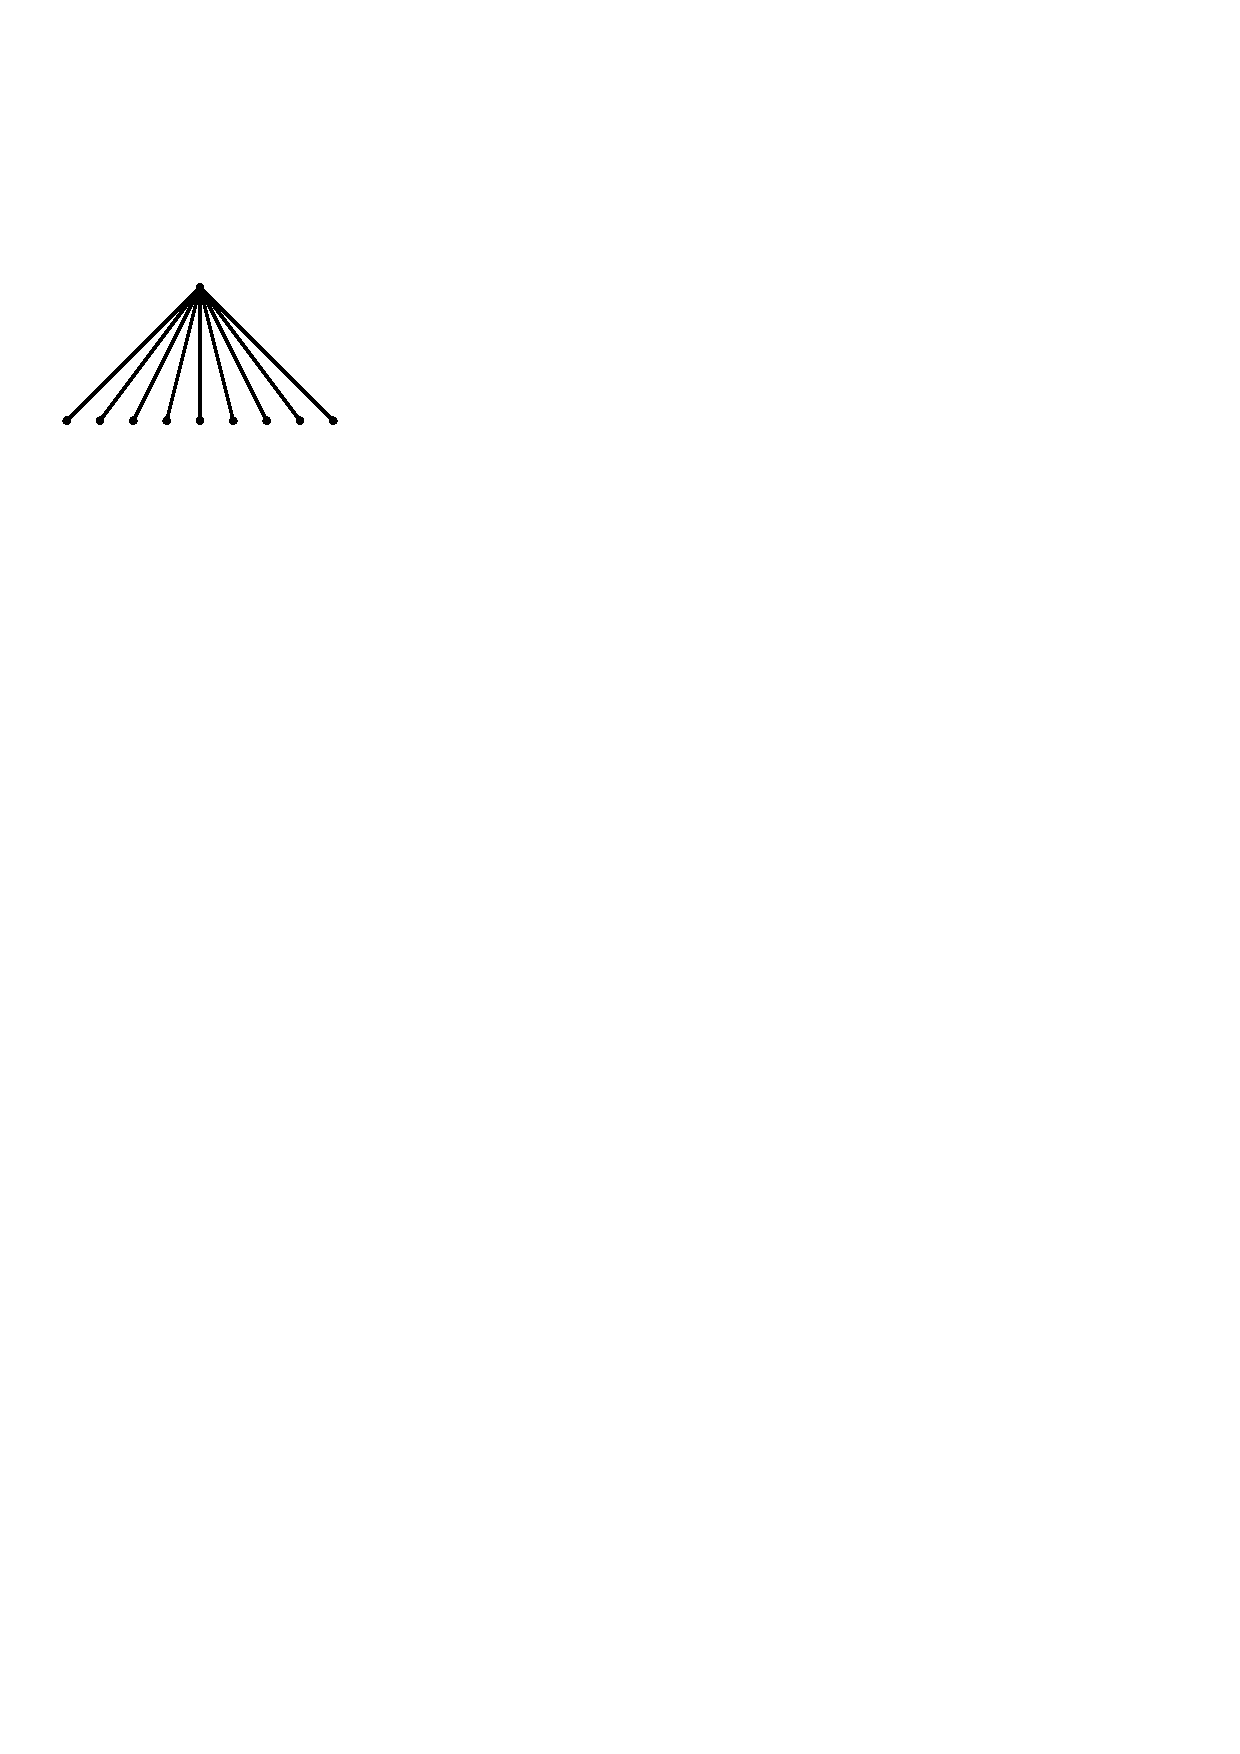
\includegraphics[width=.25\textwidth]{figs/s} & $\CartProd$ & 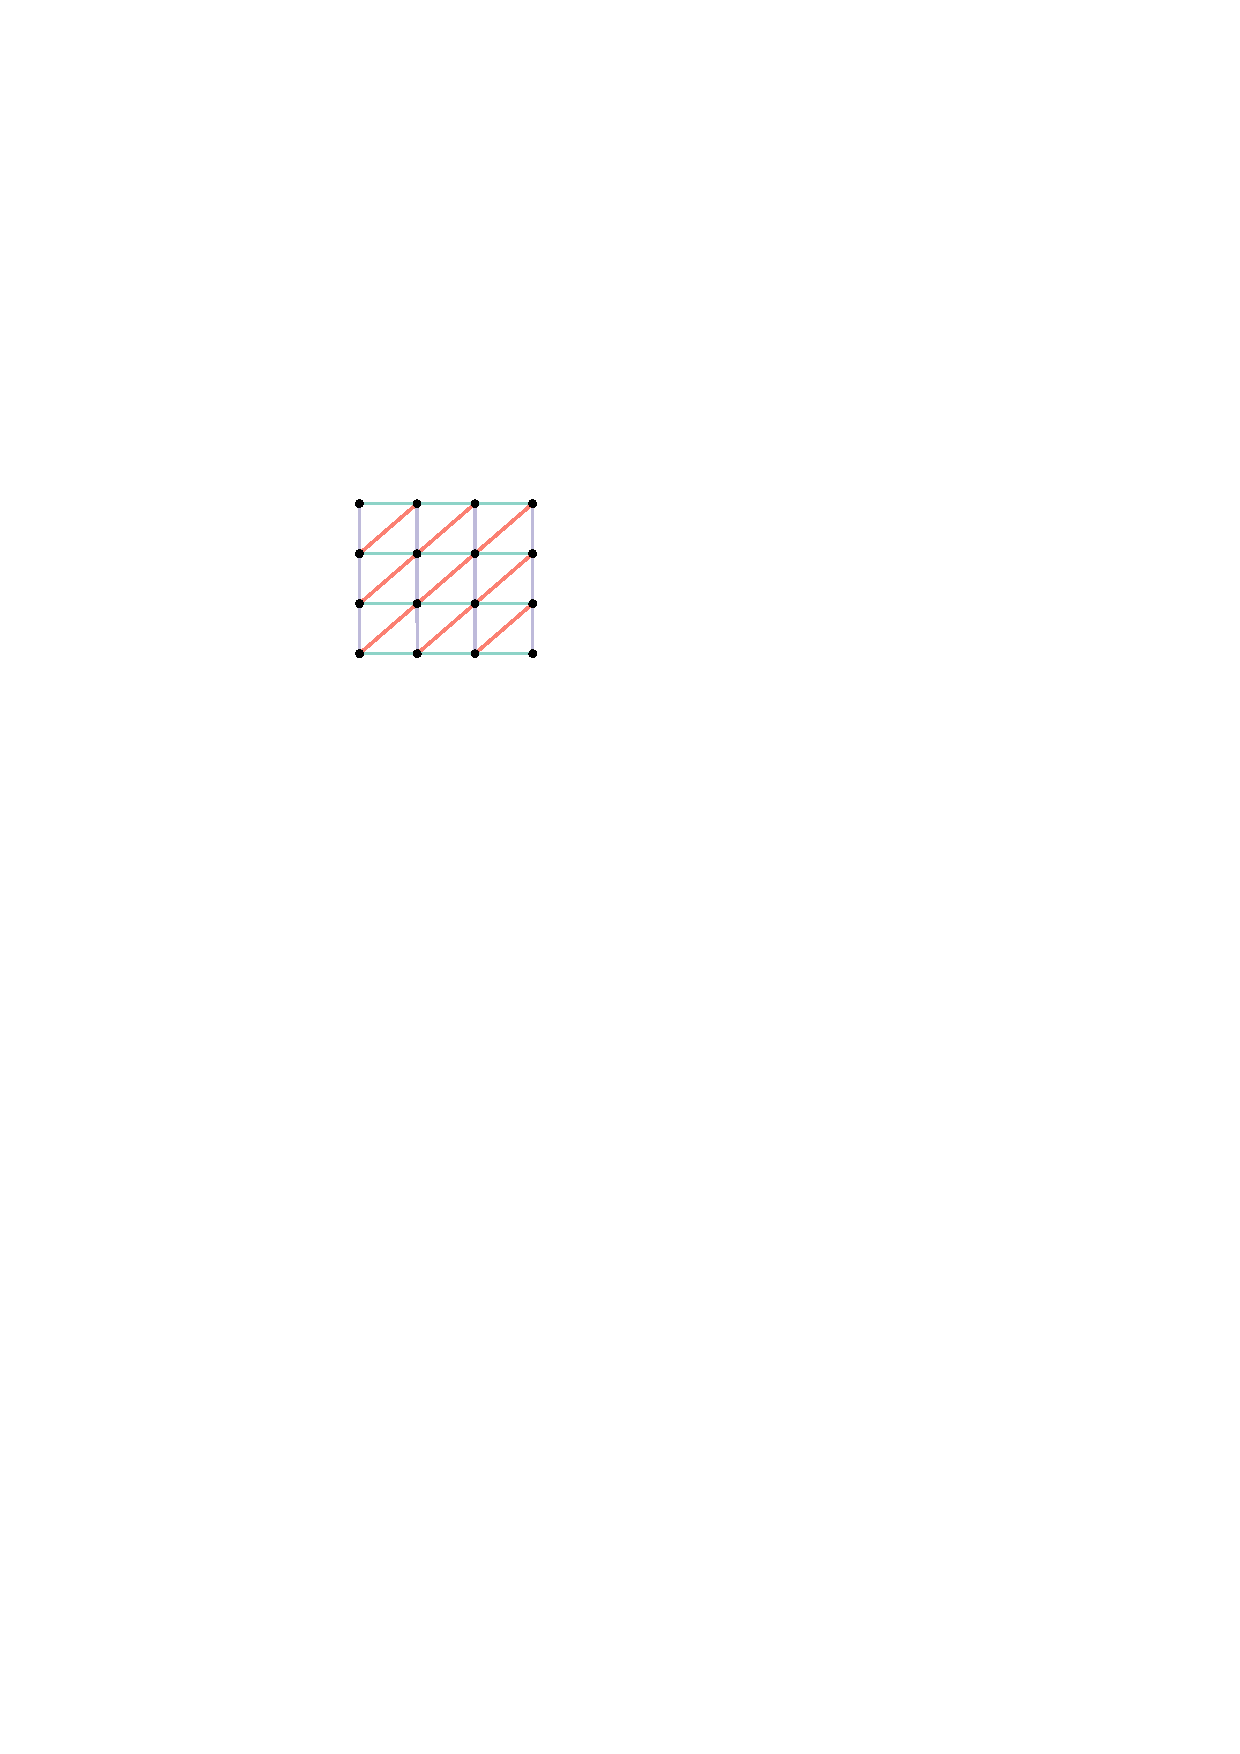
\includegraphics[width=.25\textwidth]{figs/q} & $=$
			& 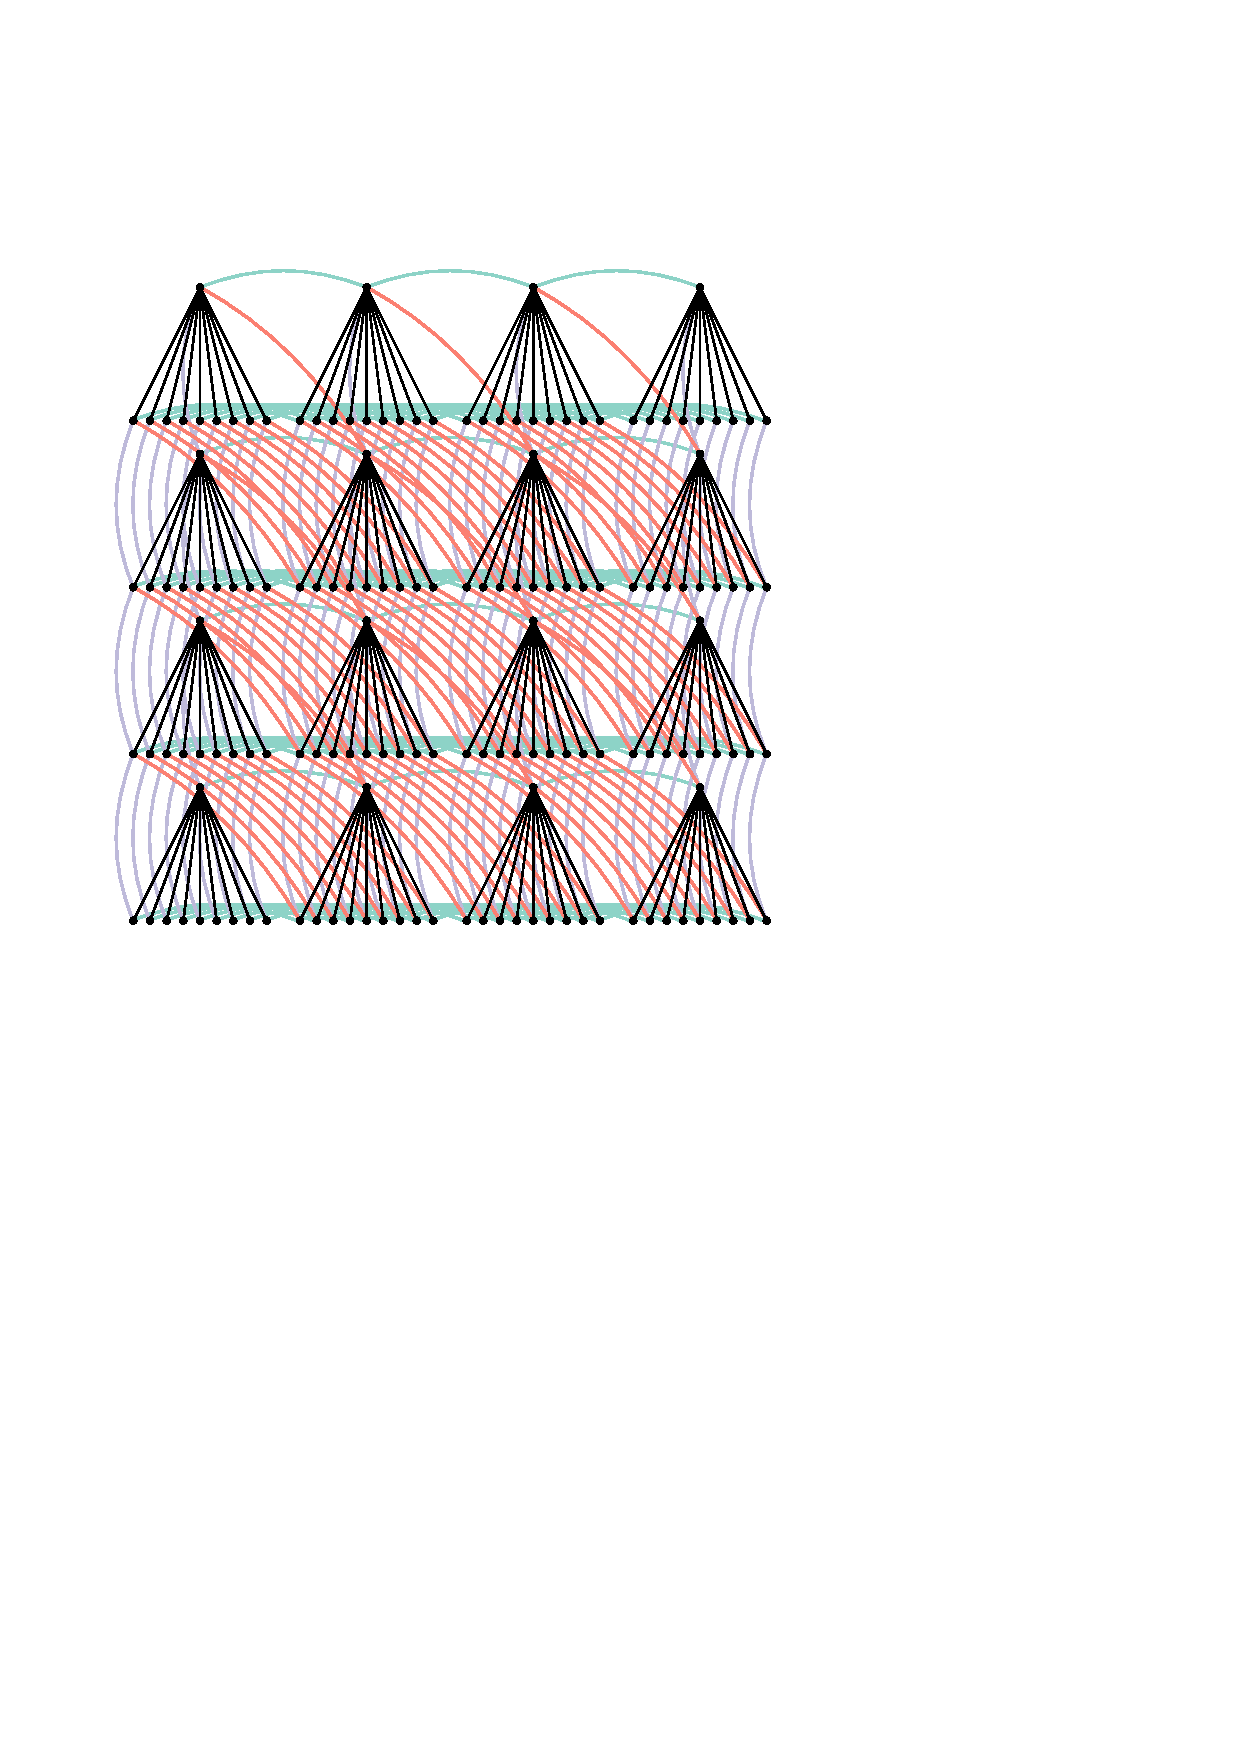
\includegraphics[width=.3\textwidth]{figs/product}
		\end{tabular}
	\end{center}
	% 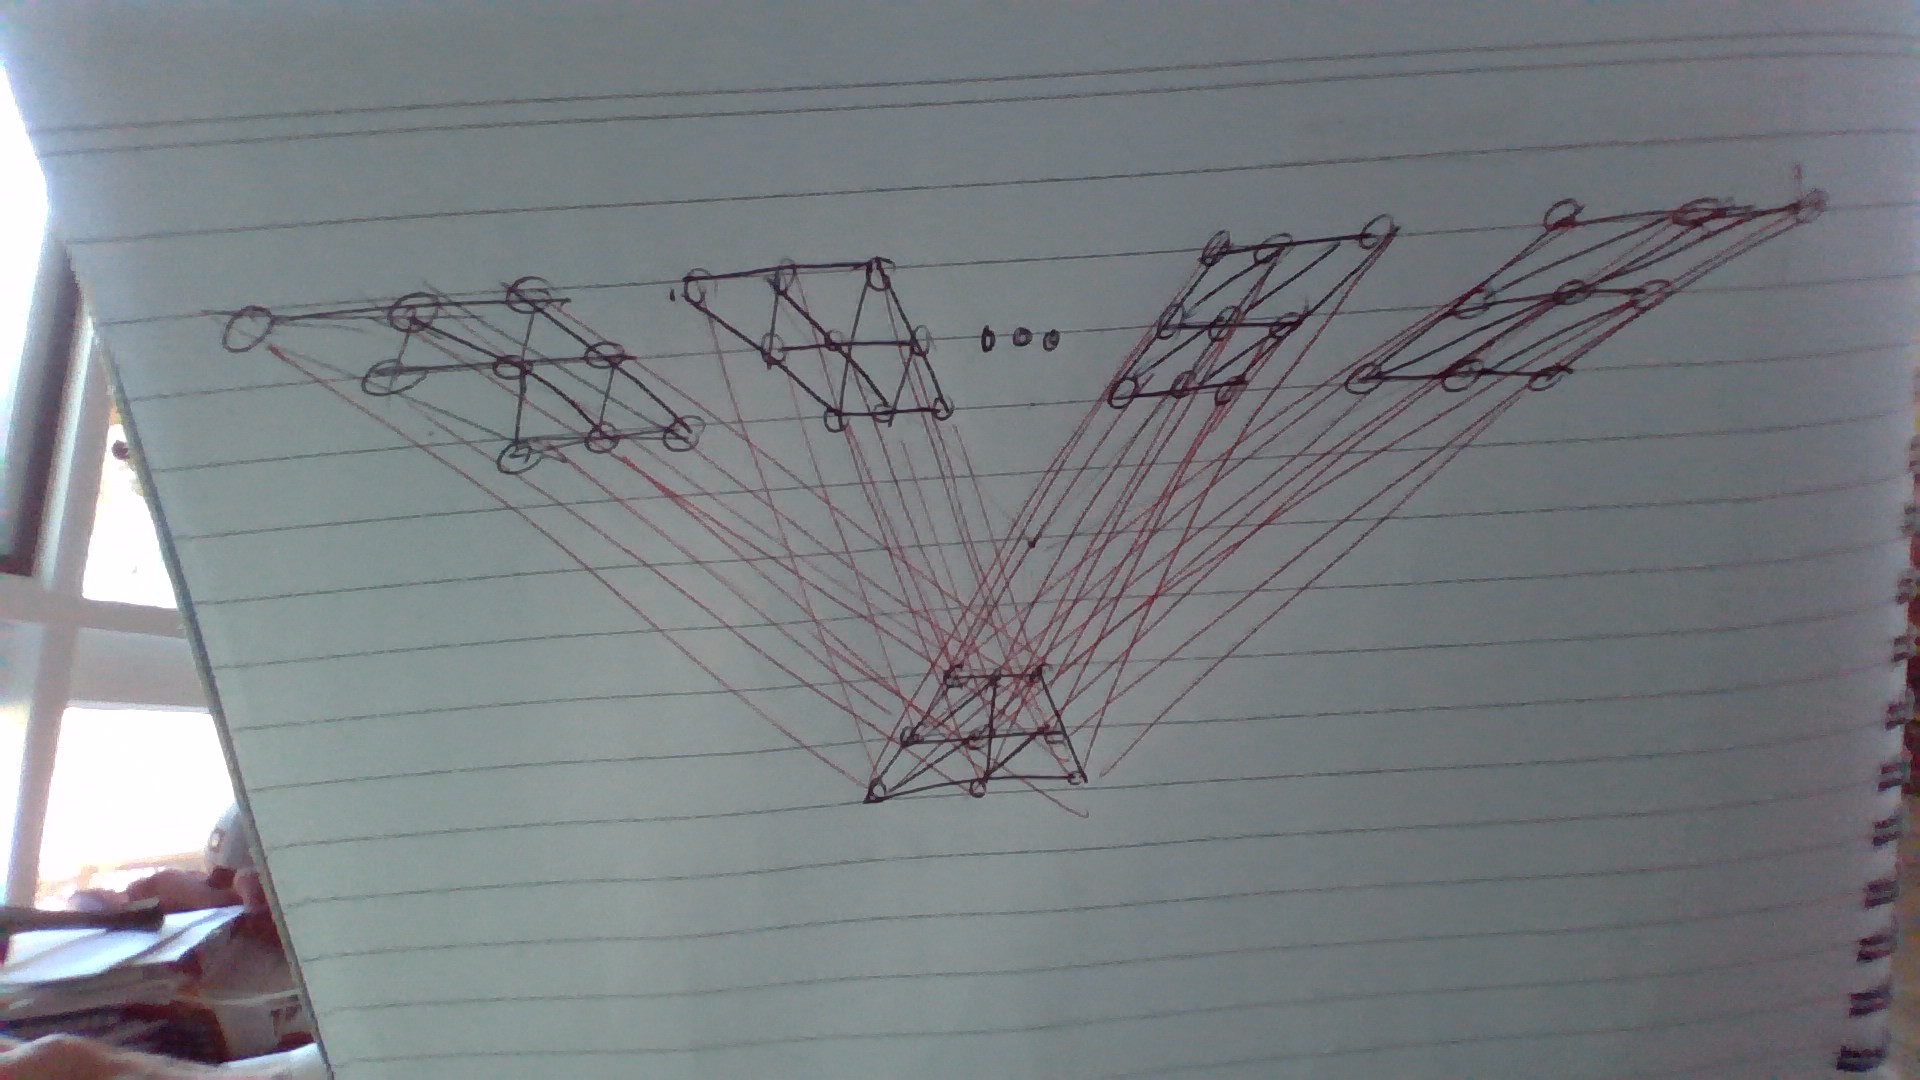
\includegraphics[width=\textwidth]{figs/figure}
	\caption{$S_9 \CartProd H_4$.}
	\label{graph}
\end{figure}


\subsection*{Subdivisions}

A noteworthy consequence of \Cref{family} is that it resolves a conjecture of \citet{BO99}. A graph $G'$ is a \textit{subdivision} of a graph $G$ if $G'$ can be obtained from $G$ by replacing the edges $vw$ of $G$ by internally disjoint paths $P_{vw}$ with endpoints $v$ and $w$. If each $P_{vw}$ has exactly $k$ internal vertices, then $G'$ is the \emph{$k$-subdivision} of $G$. If each $P_{vw}$ has at most $k$ internal vertices, then $G'$ is a \emph{$(\leq k)$-subdivision} of $G$. \citet{BO99} conjectured that the stack-number of $(\leq k)$-subdivisions ($k$ fixed)  is not much less than the stack-number of the original graph. More precisely:

\begin{conj}[\citep{BO99}]
\label{B_conj}
There exists a function $f$ such that for every graph $G$ and integer $k$, if $G'$ is any $(\leq k)$-subdivision of $G$, then $\sn(G) \leq f(\sn(G’),k)$.
\end{conj}

\citet{DujWoo05} established a connection between this conjecture and the question of whether stack-number is bounded by queue-number. In particular, they showed that if
\cref{B_conj} is true, then stack-number is bounded by queue-number. Since \cref{family} shows that stack-number is not bounded by queue-number, \cref{B_conj} is false. The proof of \citet{DujWoo05} is based on the folllowing key lemma: every graph $G$ has a $3$-stack subdivision with $1+2 \ceil{\log_2\qn(G)}$ division vertices per edge. Applying this result to the graph $G=S_b\CartProd H_n$ in \cref{family},
the $5$-subdivision of $S_b\CartProd H_n$ has a $3$-stack layout. If \cref{B_conj} was true, then $\sn(S_b\CartProd H_n) \leq f( 3,5)$, contradicting \cref{family}.

%Specifically,
%\[
%    \mathcal{F} := \{ S_b\square H_n : b,n\in\N\}
%\]
%where $S_b$ denotes the star with $b$ leaves and $H_n$ is the triangulated $n\times n$ grid.

%\todo[inline]{PM: Does anyone know if there is a standard box operator that is typeset like this $S\boxtimes H$ or $S\boxdot H$ instead of like this $S\square H$ or like this $S\Box H$?  I tried square and Box. DW: I defined \texttt{CartProd} which typesets okay $A \CartProd B$	.}


%The graph $G$ in \cref{family} is obtained as follows (See \figref{graph}): Let $S_b$ denote the star graph with root $r$ and $b$ leaves.  For an even positive integer $n$, let $H_n$ be the $n\times n$ triangulated grid, defined by $V(H_n):=\{1,\ldots,n\}^2$ and
%\begin{align*}
%E(H_n) & :=\{(x,y)(x+1,y):x\in\{1,\ldots,n-1\},\,y\in\{1,\ldots,n\}\} \\
%& \qquad \cup \{(x,y)(x,y+1):x\in\{1,\ldots,n\},\,y\in\{1,\ldots,n-1\}\} \\
%& \qquad \cup \{(x,y+1)(x+1,y):x,y\in\{1,\ldots,n-1\}\} \enspace .
%\end{align*}
%We consider the graph $G:=S_b\CartProd H_n$. That is, $V(G)=V(S_b)\times V(H_n)$ where vertices $(v_1,w_1),(v_2,w_2)\in V(G)$ are adjacent whenever $v_1=w_1$ and $v_2w_2\in E(H_n)$, or $v_1w_1\in E(S_b)$ and $v_2=w_2$.


%SAY SOMETHING ABOUT THE RESULTS OF \citet{Pupyrev20}. I EXPECT WE SOLVE SOME OPEN PROBLEM HERE.\todo{PM:Not really, his open problem is about $H\boxtimes P$ where $H$ has bounded treewidth.}

\subsection*{Is Queue-number Bounded by Stack-Number? }

It remains open whether queues are more powerful than stacks; that is, whether queue-number is bounded by stack-number. Several reults are known about this problem. \citet{HLR92} showed that every 1-stack graph has a 2-queue layout. \citet{DJMMUW20} showed that planar graphs have bounded queue-number. (Note that graph products also feature heavily in this proof.)\ Since 2-stack graphs are planar, this implies that 2-stack graphs have bounded queue-number. It is open whether 3-stack graphs have bounded queue-number. In fact, the case of three stacks is as hard as the general question. \citet{DujWoo05} proved that queue-number is bounded by stack-number if and only if 3-stack graphs have bounded queue-number. Moreover, if this is true then stack-number is bounded by a polynomial function of queue-number.


\section{Stack and Queue Layouts of Cartesian Products}

\todo[inline]{Add discussion of result of \citet{BK79}: $\sn(G\CartProd H) \leq \sn(G) + \dsn(H)$ for bipartite $H$. Highlight the key difference between stack and queue layouts is that we need $H$ to be bipartite here.}

\todo{mention results of \citet{Pupyrev20} about bipartite graphs?}

First we prove that $\qn(S_b\CartProd H_n)\leq 4$, as claimed in \cref{family}. We need the following definition due to \citet{Wood-Queue-DMTCS05}. A queue layout $(\varphi,\prec)$ is \emph{strict} if for every vertex $u\in V(G)$ and for all neighbours $v,w\in N_G(u)$, if $u\prec v,w$ or $v,w \prec u$, then $\varphi(uv)\neq \varphi(uw)$. Let $\sqn(G)$ be the minimum integer $k$ such that $G$ has a strict $k$-queue layout. To see that $\sqn(H_n) \leq 3$, order the vertices row-by-row and then left-to-right within a row, with vertical edges in one queue, horizontal edges in one queue, and diagonal edges in another queue.
\citet{Wood-Queue-DMTCS05} proved that $\qn(G\CartProd H) \leq \qn(G) + \sqn(H)$ for all graphs $G$ and $H$. Of course, $S_b$ has a 1-queue layout (since no two edges are nested for any vertex-ordering). Thus $\qn(S_b \CartProd H_n)\leq 4$.

\section{The Main Proof}

We now turn to the proof of our main result, the lower bound on $\sn(G)$, where $G:= S_b\CartProd H_n$. Consider a hypothetical $s$-stack layout $(\varphi,\prec)$ of $G$ where $n$ and $b$ are chosen sufficiently large compared to $s$ as detailed below. We begin with three lemmata that, for sufficiently large $b$, provide a large subgraph $S_d$ of $S_b$ for which the induced stack layout of $S_d\CartProd H_n$ is highly structured.

For each node $v$ of $S_b$, define $\pi_v$ as the permutation of $\{1,\ldots,n\}^2$ in which $(x_1,y_1)$ appears before $(x_2,y_2)$ if and only if $(v,(x_1,y_1))\prec (v,(x_2,y_2))$. The following lemma is an immediate consequence of the Pigeonhole Principle:

\begin{lem}\lemlabel{uniform_order}
    There exists a permutation $\pi$ of $\{1,\ldots,n\}^2$ and a set $L_1$ of leaves of $S_b$ of size $a\ge b/(n^2)!$ such that $\pi_{v}=\pi$ for each $v\in L_1$.
\end{lem}

% \todo[inline]{If we cared, we could improve this to $b/2^{cn^2}$ since we only use the weaker property (P3) in the final proof. DW: I don't care. }

For each leaf $v$ in $L_1$, let $\varphi_v$ be the edge colouring of $H_n$ defined by $\varphi_v(xy):=\varphi((v,x)(v,y))$ for each $xy\in E(H_n)$. Since $H_n$ has maximum degree $6$ and is not 6-regular, it has fewer than $3n^2$ edges.  Therefore there are fewer than $s^{3n^2}$ edge colourings of $H_n$ using $s$ colours.  Another application of the Pigeonhole Principle proves the following:

\begin{lem}\lemlabel{uniform_colour}
    There exists a subset $L_2\subseteq L_1$ of size $c\ge a/s^{3n^2}$
    and an edge colouring $\phi:E(H_n)\to\{1,\ldots,s\}$ such that $\varphi_v=\phi$ for each $v\in L_2$.
\end{lem}


Let $S_{c}$ be the subgraph of $S_b$ induced by $L_2\cup\{r\}$. The preceding two lemmata ensure that, for distinct leaves $v$ and $w$ of $S_{c}$, the stack layouts of the isomorphic graphs $G[\{(v,p):p\in V(H_n)\}]$ and $G[\{(w,p):p\in V(H_n)\}]$ are identical. The next lemma is a statement about the relationships between the stack layouts of $G[\{(v,p):v\in V(S_{c})\}]$ and $G[\{(v,q):v\in V(S_{c})\}]$ for  distinct $p,q\in V(H_n)$.  It does not assert that these two layouts are identical but it does state that they fall into one of two categories.

\begin{lem}\lemlabel{forward_or_backward}
    There exists a sequence $L_3:=u_1,\ldots,u_{d}$ with $\{u_1,\ldots,u_{d}\}\subseteq L_2$ of length $d\ge c^{1/2^{n^2-1}}$ such that, for each $p\in V(H_n)$, either  $(u_1,p)\prec (u_2,p)\prec\cdots\prec (u_{d},p)$ or $(u_1,p)\succ (u_2,p)\succ\cdots\succ (u_{d},p)$.
\end{lem}

\begin{proof}
    Let $p_1,\ldots,p_{n^2}$ denote the vertices of $H_n$ in any order.
    Begin with the sequence $S_1:=v_{1,1},\ldots,v_{1,c}$ that contains all $c$ elements of $L_2$ ordered so that $(v_{1,1},p_1)\prec\cdots\prec(v_{1,c},p_1)$.  For each $i\in\{2,\ldots,n^2\}$, the Erd\H{o}s-Szekeres Theorem~\citep{ES35} implies that $S_{i-1}$ contains a subsequence $S_i:=v_{i,1},\ldots,v_{i,|S_i|}$ of length $|S_i|\ge \sqrt{|S_{i-1}|}$ such that $(v_{i,1},p_i)\prec\cdots\prec(v_{i,|S_i|},p_i)$ or $(v_{i,1},p_i)\succ\cdots\succ(v_{i,|S_i|},p_i)$.  It is straightforward to verify by induction on $i$ that $|S_i| \ge c^{1/2^{i-1}}$ resulting in a final sequence $S_{n^2}=:L_3$ of length at least $c^{1/2^{n^2-1}}$.
\end{proof}

For the rest of the proof we will work with the star $S_d$ whose leaves are $u_1,\ldots,u_d$ described in \lemref{forward_or_backward}.  Consider the (improper) vertex colouring of $H_n$ obtained by colouring each vertex $p\in V(H_n)$ \emph{red} if $(u_1,p)\prec\cdots\prec (u_d,p)$ and colouring $p$ \emph{blue} if $(u_1,p)\succ\cdots\succ(u_d,p)$. We need the following famous Hex Lemma~\citep{Gale79}.

\begin{lem}[\citep{Gale79}] \label{hex_lemma}
Every red--blue vertex colouring of the graph $H_n$	contains an $n$-vertex path $R$ consisting entirely of red vertices or entirely of blue vertices.
\end{lem}

%\begin{proof}
%    The dual of $H_n$ is the board on which the game Hex is played.  The well-known \emph{Hex Lemma} states that any colouring of the vertices of $H_n$ with colours red and blue contains exactly one of the following \cite{Gale79}:
%    \begin{compactenum}
%        \item a path with endpoints $(x,1)$ and $(x',n)$ consisting entirely of red vertices, for some $x,x'\in\{1,\ldots,n\}$; or
%        \item a path with endpoints $(1,y)$ and $(n,y')$ consisting entirely of blue vertices, for some $y,y'\in\{1,\ldots,n\}$.
%    \end{compactenum}
%    In either case, the path contains at least $n$ vertices and therefore has a $n$-vertex subpath consisting entirely of red vertices or entirely of blue vertices.
%\end{proof}

Without loss of generality, assume that the path $R:=p_1,\ldots,p_n$ defined by \cref{hex_lemma} (with the above-defined colouring) consists entirely of red vertices, so that $(u_1,p_j)\prec\cdots\prec (u_d,p_j)$ for each $j\in\{1,\ldots,n\}$.  Recall that $(\varphi,\prec)$ is a hypothetical $s$-stack layout of $G$ and therefore it is also an $s$-stack layout of the subgraph $X:=S_d\CartProd R$. In particular, there is no set of greater than $s$ pairwise crossing edges in $X$. The following result finishes the proof by showing that such a set exists when $n> 2s$ and $d\ge (s+1)2^{n}$ (which is implied if $n=2s+1$ and $b \ge (n^2)!\, s^{3n^2}\, ((s+1)2^n)^{2^{n^2-1}} $).


\begin{lem}\lemlabel{twister}
    The graph $X$ contains a set of edges of size at least $\min\{\lfloor d/2^{n}\rfloor,\lceil n/2\rceil\}$ that are pairwise crossing with respect to $\prec$.
\end{lem}

\begin{proof}
	Extend the total order $\prec$ onto a partial order over subsets of $V(G)$ so that, for $V,W\subseteq V(G)$,  $V\prec W$ if and only if $v\prec w$ for each $v\in V$ and each $w\in W$.  We abuse notation slightly by using $\prec$ to compare elements of $V(G)$ and subsets of $V(G)$ so that, for $v\in V(G)$ and $V\subseteq V(G)$, $v\prec V$ denotes $\{v\}\prec V$.
    We will define sets $A_1\supseteq \cdots\supseteq A_{n}$ of leaves of $S_d$ so that each $A_i$ satisifies the following conditions:
    \begin{compactenum}[(C1)]
        \item $A_i$ contains $d_i\ge d/2^{i-1}$ leaves of $S_d$.
        \item Each leaf $v\in A_i$ defines an $i$-element vertex set $Z_{i,v}:=\{(v,p_j):j\in\{1,\ldots,i\}\}$.  For any distinct $v,w\in A_i$, the sets $Z_{i,v}$ and $Z_{i,w}$ are \emph{separated} with respect to $\prec$; that is, $Z_{i,v}\prec Z_{i,w}$ or $Z_{i,v}\succ Z_{i,w}$.
    \end{compactenum}

    Before defining $A_1,\ldots,A_n$ we first show how the existence of the set $A_n$ implies the lemma.  To avoid triple-subscripts, let $d':=d_n\ge d/2^{n-1}$.   The set $A_n$ defines vertex sets $Z_{n,v_1}\prec\cdots\prec Z_{n,v_{d'}}$.  Refer to \figref{twister}. Recall that $r$ is the root of $S_b$ so it is adjacent to each of $v_{1},\ldots,v_{d'}$ in $S_d$.  Therefore, for each $j\in\{1,\ldots,n\}$ and each $i\in\{1,\ldots,d'\}$, the edge $(r,p_j)(v_i,p_j)$ is in $X$. Therefore, $(r,p_j)$ is adjacent to an element of each of $Z_{n,v_1},\ldots,Z_{n,v_{d'}}$.
	\begin{figure}
		\begin{center}
			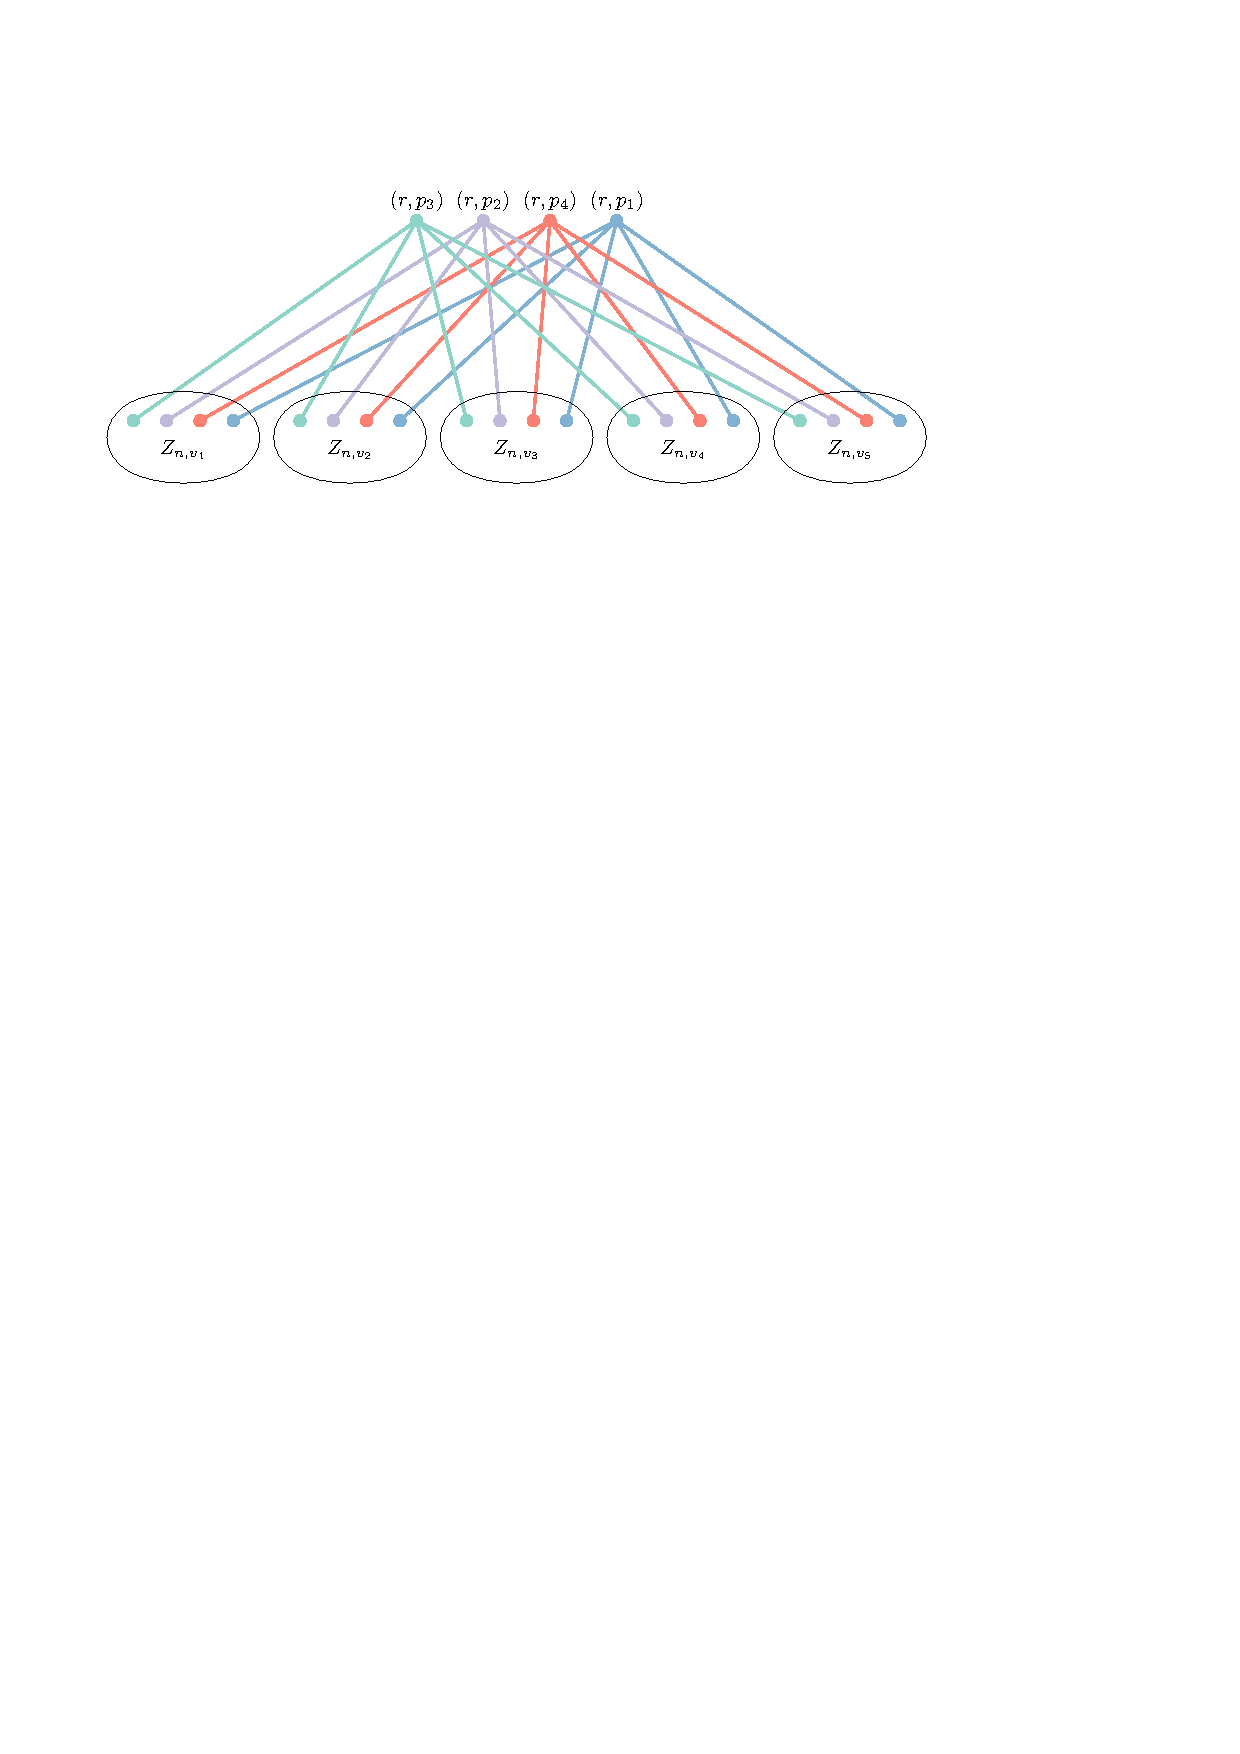
\includegraphics{figs/twister}
		\end{center}
		\caption{The sets $Z_{n,v_1},\ldots,Z_{n,v_{d'}}$ ($n=4$, $d'=5$).}
		\figlabel{twister}
	\end{figure}

    Since $Z_{n,v_1},\ldots,Z_{n,v_{d'}}$ are separated with respect to $\prec$, when viewed from afar, this situation looks like a complete bipartite graph $K_{n,d'}$ with the root vertices $L:=\{(r,p_j):j\in\{1,\ldots,n\}\}$ in one part and the groups $R:=Z_{n,v_1}\cup\cdots\cup Z_{n,v_{d'}}$ in the other part.  Any linear ordering of $K_{n,d'}$ has a large set of pairwise crossing edges so, intuitively, the induced subgraph $X[L\cup R]$ should also have a large set of pairwise crossing edges. We can formalize this as follows: Label the vertices in $L$ as $r_1,\ldots,r_n$ so that $r_1\prec \cdots\prec r_{n}$.  Then at least one of the following two cases applies (see \figref{median}):
    \begin{enumerate}
        \item $Z_{n,\lfloor d'/2\rfloor}\prec r_{\lceil n/2\rceil}$ in which case the graph between $r_{\lceil n/2\rceil},\ldots,r_{n}$ and $Z_{n,1},\ldots,Z_{n,\lfloor d'/2\rfloor}$ has a set of at least $\min\{\lfloor d'/2\rfloor,\lceil n/2\rceil\}$ pairwise-crossing edges.
        \item $r_{\lceil n/2\rceil}\prec Z_{\lceil d'/2\rceil+1}$ in which case the graph between $r_1,\ldots,r_{\lceil n/2\rceil}$ and $Z_{\lceil d'/2\rceil+1},\ldots,Z_{d'}$ has a set of $\min\{\lfloor d'/2\rfloor,\lceil n/2\rceil\}$ pairwise-crossing edges.
    \end{enumerate}
	\begin{figure}
		\begin{center}
			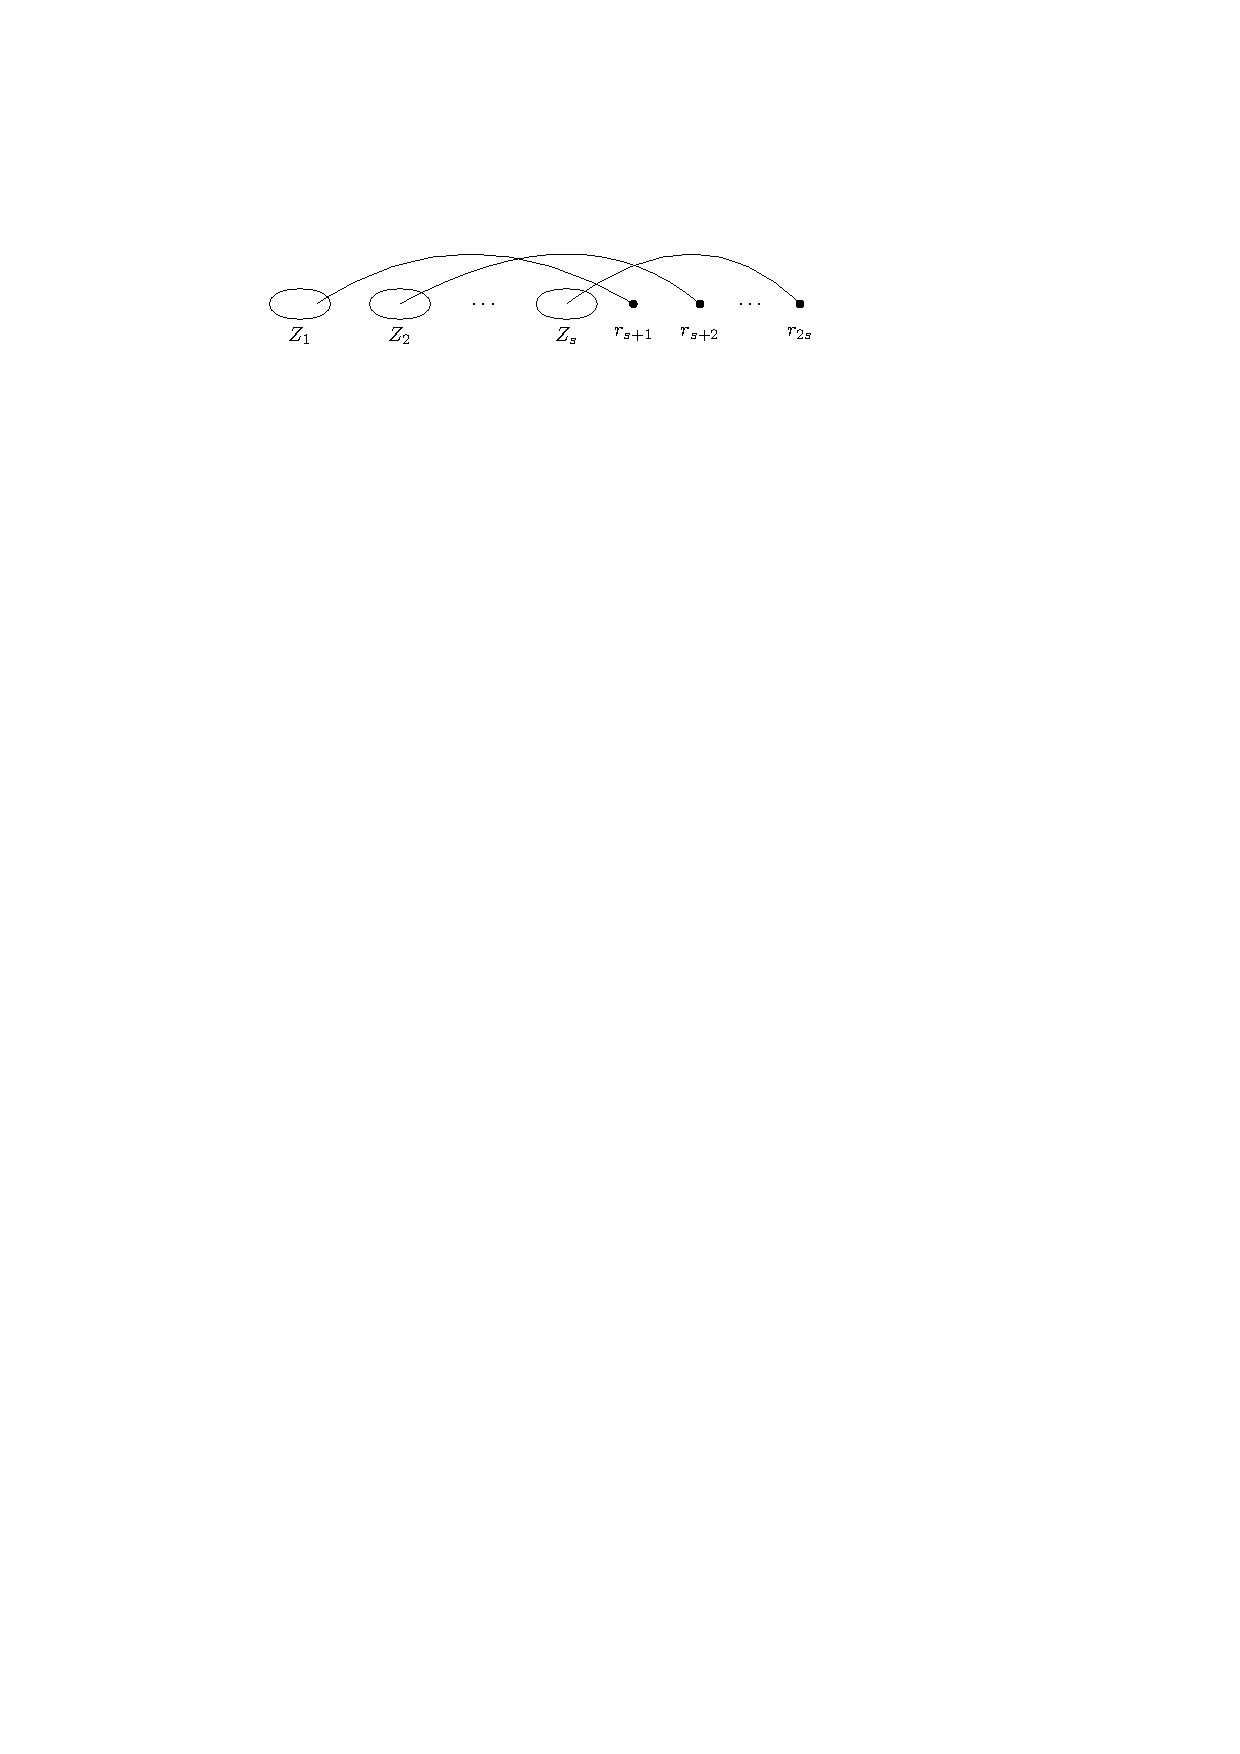
\includegraphics{figs/median-1} \\ 1 \\[2em]
			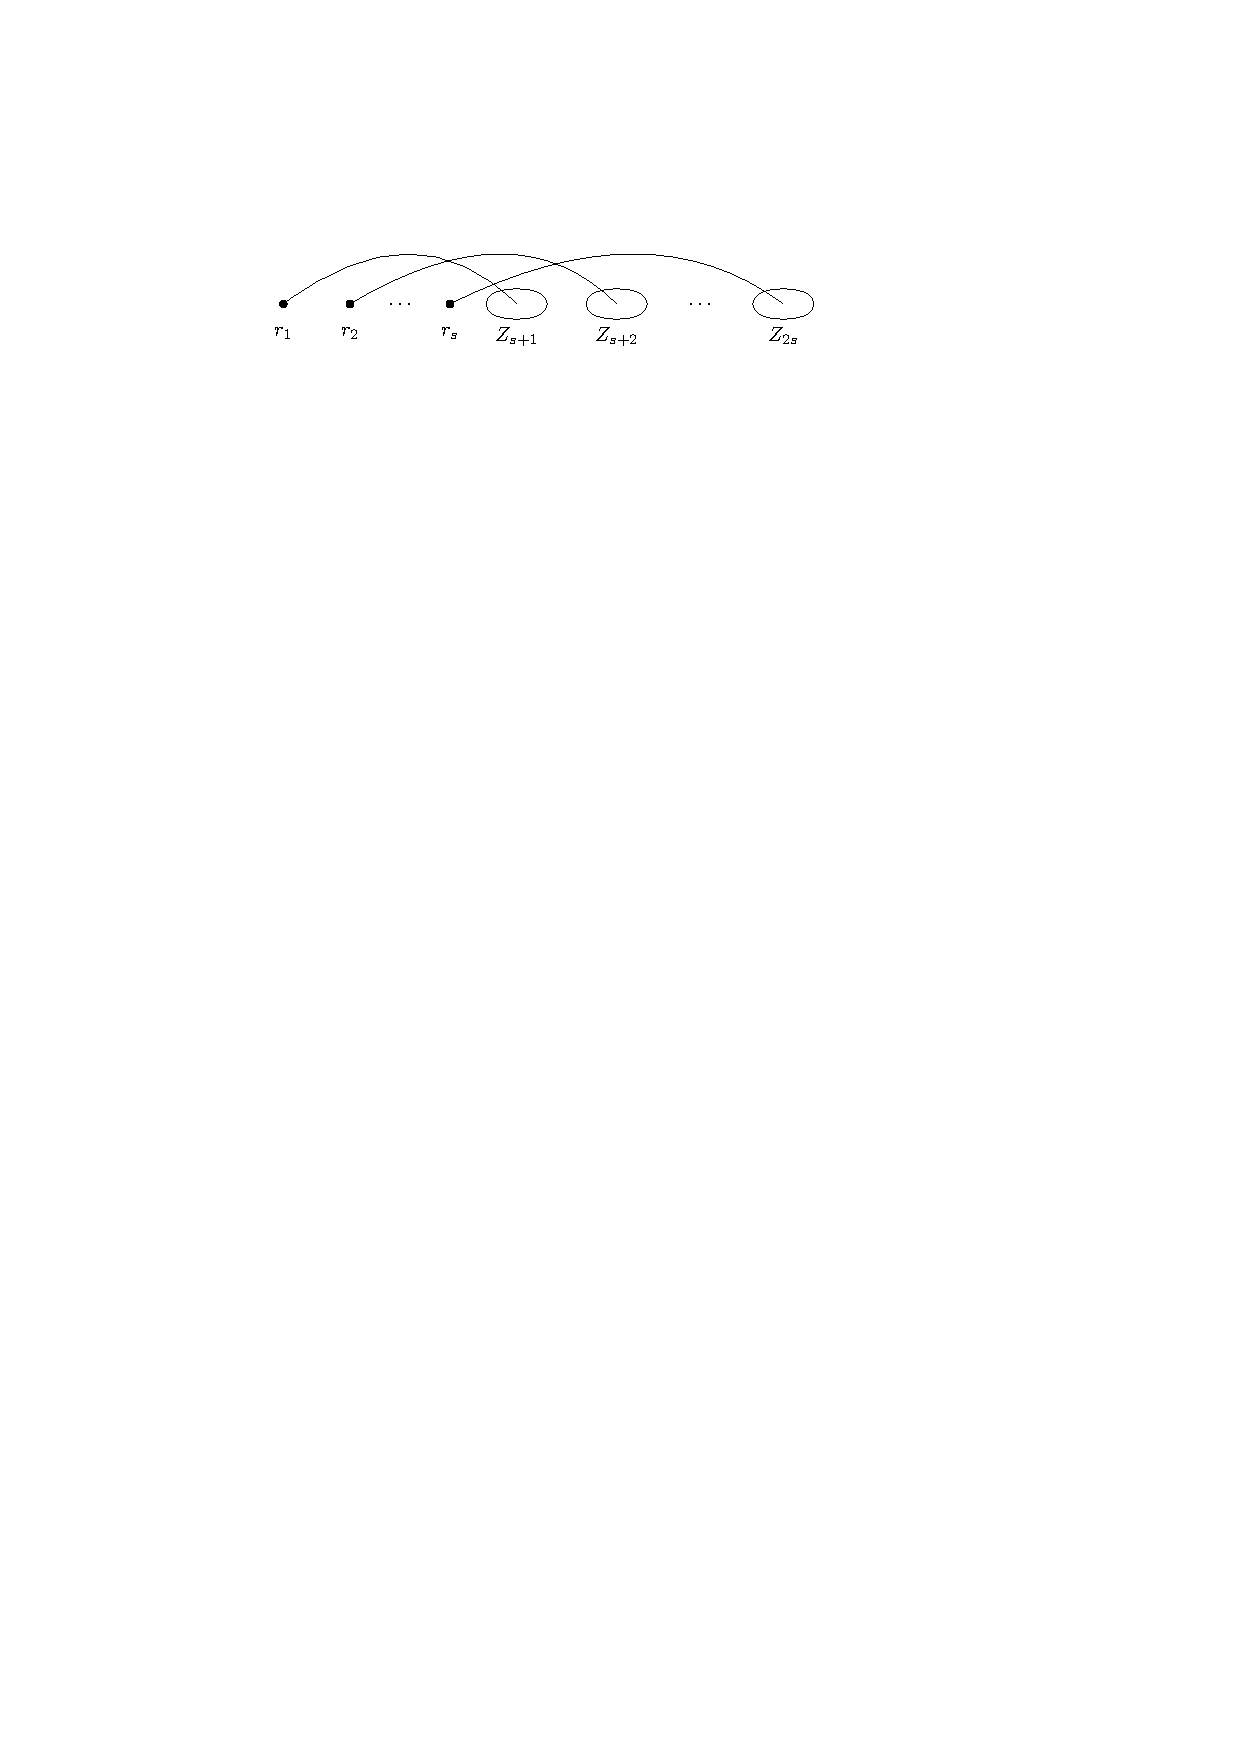
\includegraphics{figs/median-2} \\ 2
		\end{center}
		\caption{The two cases in the proof of \lemref{twister}.}
		\figlabel{median}
	\end{figure}
	Since, by (C1), $d'\ge d/2^{n-1}$, either case results in a set of pairwise-crossing edges of size at least $\min\{\lfloor d/2^n\rfloor,\lceil n/2\rceil\}$, as claimed.

    All that remains is to define the sets $A_1\supseteq\cdots\supseteq A_n$ that satisfy (C1) and (C2).  Let $A_1$ be the set of all the leaves of $S_d$.  For each $i\in\{2,\ldots,n\}$, the set $A_i$ is defined as follows:  Let $Z_1,\ldots,Z_{|A_{i-1}|}$ denote the sets $Z_{i-1, v}$ for each $v\in A_{i-1}$ ordered so that $Z_1\prec\cdots\prec Z_{|A_{i-1}|}$. By Property (C2), this is always possible.	Label the vertices of $A_{i-1}$ as $v_1,\ldots,v_{|A_{i-1}|}$ so that $(v_1,p_{i-1})\prec\cdots\prec (v_r,p_{i-1})$.   (This is equivalent to naming them so that $(v_j,p_{i-1})\in Z_j$ for each $j\in\{1,\ldots,|A_{i-1}|\}$.)  Define the set $A_i:=\{v_{2k+1}:k\in\{0,\ldots,\lfloor(|A_{i-1}|-1)/2\rfloor\}\}=\{v_{j}\in A_{i-1}:\text{$j$ is odd}\}$.  This completes the definition of $A_1,\ldots,A_n$.

	All that remains is to verify that $A_i$ satisfies (C1) and (C2) for each $i\in\{1,\ldots,n\}$.  We do this by induction on $i$. The base case $i=1$ is trivial so we assume from this point on that $i\in\{2,\ldots,n\}$.   To see that $A_i$ satisfies (C1) just observe that $|A_i|=\lceil |A_{i-1}|/2\rceil \ge |A_{i-1}|/2\ge d/2^{i-1}$, where the final inequality follows by applying the inductive hypothesis $|A_{i-1}|\ge d/2^{i-2}$.  Now all that remains is to show that $A_i$ satisfies (C2).

    Recall that, for each $v\in A_{i-1}$, the edge $e_v:=(v,p_{i-1})(v,p_i)$ is in $X$.  We have the following properties:
    \begin{compactenum}[(P1)]
        \item By \lemref{uniform_colour}, $\varphi(e_v)=\phi(p_{i-1}p_i)$ for each $v\in A_{i-1}$.
        \item Since $p_{i-1}$ and $p_i$ are both red, $(v,p_{i-1})\prec (w,p_{i-1})$ if and only if $(v,p_{i})\prec (w,p_{i})$ for each $v,w\in A_{i-1}$.
        \item By \lemref{uniform_order}, $(v,p_{i-1})\prec (v,p_i)$ for every $v\in A_{i-1}$ or $(v,p_{i-1})\succ (v,p_i)$ for every $v\in A_{i-1}$.
    \end{compactenum}
    We claim that these three conditions imply that the vertex sets $\{(v,p_{i-1}):v\in A_{i-1}\}$ and $\{(v,p_i):v\in A_{i-1}\}$ interleave perfectly with respect to $\prec$. More precisely:
	\begin{clm}\clmlabel{interleave} $(v_1,p_{i-1+t})\prec (v_1,p_{i-t}) \prec (v_2,p_{i-1+t}) \prec (v_2,p_{i-t}) \cdots \prec (v_r,p_{i-1+t}) \prec (v_r,p_{i-t})$ for some $t\in\{0,1\}$.
	\end{clm}
	\begin{proof}[Proof of \clmref{interleave}]
		By (P3) we may assume, without loss of generality, that $(v,p_{i-1})\prec (v,p_i)$ for each $v\in A_{i-1}$, in which case we are trying to prove the claim for $t=0$.  Therefore, it is sufficient to show that $(v_j,p_i)\prec (v_{j+1},p_{i-1})$ for each $j\in\{1,\ldots,r-1\}$.  For the sake of contradiction, suppose $(v_j,p_{i})\succ (v_{j+1},p_{i-1})$ for some $j\in\{1,\ldots,r-1\}$. By the labelling of $A_{i-1}$,  $(v_j,p_{i-1})\prec (v_{j+1},p_{i-1})$ so, by (P2),  $(v_{j},p_i) \prec (v_{j+1},p_i)$.  Therefore
		\[
			(v_j,p_{i-1})\prec (v_{j+1},p_{i-1})\prec(v_{j},p_i) \prec
		   (v_{j+1}, p_i) \enspace .
	   	\]
		Therefore the edges $e_{v_j}=(v_j,p_{i-1})(v_j,p_{i})$ and $e_{v_{j+1}}=(v_{j+1},p_{i-1})(v_{j+1},p_i)$ cross with respect to $\prec$.  But this is a contradiction since, by (P1),  $\varphi(e_{v_j}) =\varphi(e_{v_{j+1}})=\phi(p_{i-1}p_i)$.
		This contradiction completes the proof of \clmref{interleave}.
	\end{proof}

% \todo{DW: Why are these $\prec$'s red?  PM: Just me keeping track of which one was the assumption, they don't need to be red.}

We now complete the proof that $A_i$ satisfies (C2). Apply \clmref{interleave} and assume without loss of generality that $t=0$, so that
	\[
		(v_1,p_{i-1})\prec (v_1,p_{i}) \prec (v_2,p_{i-1}) \prec (v_2,p_{i}) \cdots \prec (v_r,p_{i-1}) \prec (v_r,p_{i}) \enspace .
	\]

    For each $j\in\{1,\ldots,r-2\}$, we have $(v_{j+1},p_{i-1})\in Z_{j+1}\prec Z_{j+2}$, so  $(v_j,p_i)\prec (v_{j+1},p_{i-1}) \prec Z_{j+2}$.  Therefore $Z_j\cup\{(v_j,p_i)\} \prec Z_{j+2}$.  By a symmetric argument, $Z_j\cup\{(v_j,p_i)\} \succ Z_{j-2}$ for each  $j\in\{3,\ldots,r\}$.  Finally, since $(v_{j},p_i)\prec (v_{j+2},p_i)$ for each odd $i\in\{1,\ldots,r\}$, we have $Z_{j}\cup\{(v_j,p_i)\} \prec Z_{j+2}\cup\{(v_{j+2},p_i)\}$ for each odd $j\in\{1,\ldots,r-2\}$.  Thus $A_i$ satisifies (C2) since the sets $Z_1\cup\{(v_1,p_i)\},Z_3\cup\{(v_3,p_i)\},\ldots,Z_{2\lfloor (r-1)/2\rfloor+1} \cup (v_{2\lfloor (r-1)/2\rfloor+1},p_i)$ are precisely the sets $Z_{i,1},\ldots,Z_{i,d_i}$ determined by our choice of $A_i$.
\end{proof}

% \begin{lem}\lemlabel{twister}
%     Let $G$ be any graph, let $\prec$ be any linear ordering of $V(G)$,  let $Z_{1}\prec\cdots\prec Z_{2s}$ be subsets of $V(G)$, and let $r_1\prec\cdots\prec r_{2s}$ be vertices of $G$ such that, for each $i,j\in\{1,\ldots,2s\}$, $G$ contains an edge $r_iz_j$ with $z_j\in Z_j$. Then $G$ contains a set of $s$ edges that are pairwise crossing with respect to $\prec$. \todo[inline]{I think we should not re-use $s$ in this lemma. More importantly, do we really need Lemma 6? It could be easily merged into the proof of Lemma 5 where Lemma 6 is used, and this would avoid having to translate notation. It took me a while to realise that $r_1,\dots,r_{2s}$ corresponds to $L$ in Lemma 5.}
% \end{lem}
%
% \begin{proof}
% \end{proof}
%
\section{Open Problems}

Recall that every 1-queue graph has a 2-stack layout \citep{HLR92} and we proved that there are 4-queue graphs with unbounded stack-number. The following questions remain open: Do 2-queue graphs have bounded stack-number? Do 3-queue graphs have bounded stack-number?

Given the role of cartesian products in our proof, it is natural to ask when is $\sn(G_1\CartProd G_2)$ bounded? Note that $H_n$ is a subgraph of a planar Hamiltonian graph (namely, $H_{2n}$), so $\sn(H_n) \leq 2$. So $\sn(G_1\CartProd G_2)$ can be unbounded even when $G_1$ is a star and $\sn(G_2)\leq 2$.
Since $\sn(G_2)\leq 1$ if and only if $G_2$ is outerplanar, the following question naturally arises: Is $\sn(S \CartProd H)$ bounded for every star $S$ and outerplanar graph $H$ with bounded degree? Is $\sn(T \CartProd H)$ bounded for every tree $T$ and outerplanar graph $H$ with bounded degree? The assumption that $H$ has bounded degree is needed since $S_n \CartProd S_n$ contain the 1-subdivision of $K_{n,n}$, which has unbounded stack-number~\citep{Blankenship-PhD03}.

Since $H_n\subseteq P \boxtimes P$\todo{$\boxtimes$ is not defined} where $P$ is the $n$-vertex path, \cref{family} implies that $\sn(S\boxtimes P\boxtimes P)$ is unbounded for stars $S$ and paths $P$. It is easily seen that $\sn(S\boxtimes P)$ is bounded~\citep{Pupyrev20}. The following question naturally arises (independently asked by \citet{Pupyrev20}):
Is $\sn(T \boxtimes P)$ bounded for every tree $T$ and path $P$? We conjecture the answer is ``no''.

\let\oldthebibliography=\thebibliography
\let\endoldthebibliography=\endthebibliography
\renewenvironment{thebibliography}[1]{%
\begin{oldthebibliography}{#1}%
\setlength{\parskip}{0ex}%
\setlength{\itemsep}{0ex}%
}{\end{oldthebibliography}}

%\documentclass[kpfonts]{patmorin}
\usepackage{pat}
\usepackage{paralist,graphicx}
\usepackage{array,longtable}

\usepackage[utf8]{inputenc}
\usepackage{todonotes}

\usepackage[noabbrev,capitalise]{cleveref}
\crefname{lem}{Lemma}{Lemmas}
\crefname{thm}{Theorem}{Theorems}
\crefname{cor}{Corollary}{Corollaries}
\crefname{prop}{Proposition}{Propositions}
\crefname{conj}{Conjecture}{Conjectures}
\crefname{open}{Open Problem}{Open Problems}
\crefname{obs}{Observation}{Observations}

\crefformat{equation}{(#2#1#3)}
\Crefformat{equation}{Equation #2(#1)#3}

\usepackage[numbers,sort&compress]{natbib}
\usepackage{hypernat}
\makeatletter
\def\NAT@spacechar{~}
\makeatother

\setlength{\parskip}{1ex}
\setlength{\parindent}{0ex}

\newtheorem{property}{Property}
\newcommand{\plabel}[1]{\label{prop:#1}}
\newcommand{\pref}[1]{Property~\ref{prop:#1}}

\DeclareMathOperator{\sn}{sn}
\DeclareMathOperator{\qn}{qn}
\DeclareMathOperator{\sqn}{sqn}
\DeclareMathOperator{\dsn}{dsn}
\DeclareMathOperator{\tw}{tw}

\renewcommand{\SS}{\mathcal{S}}

\renewcommand{\le}{\leqslant}
\renewcommand{\leq}{\leqslant}
\renewcommand{\ge}{\geqslant}
\renewcommand{\geq}{\geqslant}

\newcommand{\CartProd}{\mathbin{\square}}

\title{\MakeUppercase{Stack-Number is not Bounded by Queue-Number}}

\author{%
	Vida Dujmovi\'c,\!\!%
	\thanks{School of Computer Science and Electrical Engineering,
		University of Ottawa, Ottawa, Canada (\texttt{vida.dujmovic@uottawa.ca}).
		Research supported by NSERC.}
	\,\,
	Robert Hickingbotham,\!\!%
	\thanks{School of Mathematics, Monash University, Melbourne, Australia (\texttt{robert.hickingbotham@monash.edu}).}
	\,\,
	Pat Morin,\!\!%
	\thanks{School of Computer Science, Carleton University, Ottawa, Canada (\texttt{morin@scs.carleton.ca}). Research  supported by NSERC.}
	\,\,
	David R. Wood\thanks{School of Mathematics, Monash University, Melbourne, Australia (\texttt{david.wood@monash.edu}). Research supported by the Australian Research Council.}
}

\author{TBD}

\begin{document}
\maketitle

\begin{abstract}
We describe a family of graphs with queue-number at most 4 but unbounded stack-number. This resolves open problems of Heath, Leighton and Rosenberg (1992) and Blankenship and Oporwoski (1999).
\end{abstract}

\bigskip

\section{Introduction}

Stacks and queues are fundamental data structures in computer science, but which is more powerful? In 1992, Heath, Leighton and Rosenberg~\cite{HLR92,HR92} introduced an approach for answering this question by defining the graph parameters \textit{stack-number} and \textit{queue-number} (defined below), which respectively measure the power of stacks and queues for representing graphs. The following fundamental problems, implicit in \citep{HLR92,HR92}, were made explicit by \citet{DujWoo05}\footnote{A \emph{graph parameter} is a function $\alpha$ such that $\alpha(G)\in\mathbb{R}$ for every graph $G$ and such that $\alpha(G_1)=\alpha(G_2)$ for all isomorphic graphs $G_1$ and $G_2$. A graph parameter $\alpha$ is \textit{bounded} by a graph parameter $\beta$ if there exists a function $f$ such that $\alpha(G) \leq f(\beta(G))$ for every graph $G$.}:
\begin{compactitem}
	\item Is stack-number bounded by queue-number?
	\item Is queue-number bounded by stack-number?
\end{compactitem}

If stack-number is bounded by queue-number but queue-number is not bounded by stack-number, then stacks would be considered to be more powerful than queues. Similarly, if the converse holds, then queues would be considered to be more powerful than stacks. Despite extensive research on stack- and queue-numbers, these fundamental questions have remained unsolved.

We now formally define stack- and queue-number.
Let $G$ be a graph and let $\prec$ be a total order on $V(G)$.  Two disjoint edges $vw,xy\in E(G)$ with $v\prec w$ and $x\prec y$ \emph{cross} with respect to $\prec$ if $v\prec x\prec w\prec y$ or $x\prec v\prec y\prec w$, and \emph{nest} with respect to $\prec$ if $v\prec x\prec y\prec w$ or $x\prec v\prec w\prec y$.
%A set of $k$ pairwise nested edges is called a \emph{$k$-rainbow} and a set of $k$ pairwise crossing edges is called a \emph{$k$-twist}. A set of $k$ edges, no pair of which nest and no pair of which cross is called a \emph{hopper}.
Let $\varphi:E(G)\to\{1,\ldots,k\}$ for some integer $k\ge 1$.  Then $(\prec,\varphi)$ is a \emph{$k$-stack layout} of $G$ if, for every pair of edges $vw,xy\in E(G)$, if $\varphi(vw) = \varphi(xy)$ then $vw$ and $xy$ do not cross.\todo{PM: Suggestion: Replace second if then with $\varphi(vw)\neq\varphi(xy)$ or $vw$ and $xy$ do not cross.} Similarly, the pair $(\prec,\varphi)$ is a \emph{$k$-queue layout} of $G$ if, for every pair of edges $vw,xy\in E(G)$, if $\varphi(vw)=\varphi(xy)$ then  $vw$ and $xy$ do not nest. The smallest integer $s$ for which $G$ has an $s$-stack layout is called the \emph{stack-number} of $G$, denoted  $\sn(G)$. The smallest integer $q$ for which $G$ has a $q$-queue layout is called the \emph{queue-number} of $G$, denoted $\qn(G)$. Note that stack layouts are equivalent to book embeddings (first defined by \citet{Ollmann73}), and stack-number is also known as \emph{page-number}, \emph{book-thickness} or \emph{fixed outer-thickness}. See \citep{BK79,DujWoo04,DujWoo-DCG07,DJMMUW20,DFP13,BFGMMRU19,Yannakakis89,Yann20,MBKPRU20} and the references therein for work on stack- and queue-layouts.

Given a $k$-stack layout $(\prec,\varphi)$ of a graph $G$, for each $i\in\{1,\dots,k\}$, the set $\varphi^{-1}(i)$ behaves like a stack, in the sense that each edge $vw \in \varphi^{-1}(i)$ with $v\prec w$ corresponds to an element in a sequence of stack operations, such that if we traverse the vertices in the order of $\prec$, then $vw$ is pushed onto the stack at $v$ and popped off the stack at $w$. Similarly, each set $\varphi^{-1}(i)$ in a queue layout  behaves like a queue. In this way, the stack-number and queue-number  respectively measure the power of stacks and queues to represent graphs.


\subsection*{Is Stack-Number Bounded by Queue-number?}

This paper considers the first of the above questions. In a positive direction, \citet{HLR92}  showed that every 1-queue graph has a $2$-stack layout. On the other hand, they described graphs that need exponentially more stacks than queues. In particular, $n$-vertex ternary hypercubes have queue-number $O(\log n)$ and stack-number $\Omega(n^{1/9-\epsilon})$ for any $\epsilon>0$.

%Note that, in an $s$-stack layout, $(\prec,\varphi)$, $\varphi$ is a proper $s$-colouring of the auxilliary graph $H$ with vertex set $V(H)=E(G)$ and in which the edge $ef$ if present if and only if $e$ and $f$ cross with respect to $\varphi$.  Any $k$-twist in $G$ with respect to $\prec$ corresponds to a $k$-clique $H$.  Since the chromatic number of any graph is bounded by its clique number, the following observation is trivial:

%\begin{obs}\obslabel{no-s-twist}
%If $(\prec,\varphi)$ is an $s$-stack layout of a graph $G$ then $E(G)$ does not contain any $k$-twist for any $k>s$.
%\end{obs}

%We now formally define stack and queue layouts of graphs. Let $G=(V,E)$ be a graph with disjoint edges $vw, xy$ and a linear ordering $\leq$ of the vertices. Without loss of generality, we may assume that $v < w$, $x <y$ and $v < x$. We say that $vw$ and $xy$ \textit{cross} if $v<x<w<y$,  \textit{nest} if $v <x <y < w$, and are \textit{disjoint} if $v <w<x<y$. \todo{DW: Do we  need ``disjoint''?} A \textit{stack} is a set of pairwise non-crossing edges and a \textit{queue} is a set of pairwise non-nesting edges. A $k$-queue layout of $G$ consist of a linear ordering $\leq$ of its vertices and a partition $E_1,E_2, \dots, E_k$, of its edges into queues with respect to $\leq$. The stack-number of a graph $G$, $\sn(G)$, is the minimum integer $k$ such that $G$ has a $k$-stack layout. Similarly, the queue-number of a graph $G$, $\qn(G)$, is the minimum integer $k$ such that $G$ has a $k$-queue layout. We note that stack layouts of graphs are related to book embeddings of graph and that stack-number is also known as \textit{page-number}, \textit{book-thickness}, or \textit{fixed outer-thickness}.

%Note that stacks and queues are closely related to breadth-first search (BFS) and depth-first search (DFS) layouts of graphs. It can be easily shown that a BFS vertex ordering of a tree admits a $1$-queue layout and a DFS vertex ordering of a tree admits a $1$-stack layout.

%\citet{HLR92} showed that every 1-queue graph has a 2-stack layout. \citet{HLR92} showed that the ternary hypercubes requires exponentially more stacks than queues. In particular, $n$-vertex ternary hypercubes have queue-number at most $2 \log_3 n$, but stack-number at least $\Omega(n^{1/9-\epsilon})$ for any $\epsilon>0$. We prove the following theorem, which shows that stack-number is not bounded by queue-number.

Our key contribution is the following theorem, which shows that stack-number is not bounded by queue-number. This demonstrates that stacks are not more powerful than queues for representing graphs.

\begin{thm}\label{family}
	%  There exists a family $\mathcal{F}$ of graphs for which $\qn(G)\le 4$ for every $G\in\mathcal{F}$, and for every $s\in\N$, there exists $G\in\mathcal{F}$ for which $\sn(G)>s$.
	For every $s\in \N$ there exists a graph $G$ with $\qn(G)\le 4$ and $\sn(G)>s$.
\end{thm}

As illustrated in \cref{graph}, the graph $G$ in \cref{family} is the cartesian product\footnote{For graphs $G_1$ and $G_2$, the \emph{cartesian product} $G_1\CartProd G_2$ is the graph with vertex set $\{(v_1,v_2): v_1 \in V(G_1), v_2 \in V(G_2)\}$, where $(v_1,v_2)(w_1,w_2)\in E(G_1\CartProd G_2)$ if $v_1=w_1$ and $v_2w_2\in E(G_2)$, or $v_1w_1\in E(G_1)$ and $v_2=w_2$.} $S_b\CartProd H_n$, where $S_b$ is the star graph with root $r$ and $b$ leaves, and $H_n$ is the dual of the hexagonal grid, defined by
\begin{align*}
V(H_n)  :=\{1,\ldots,n\}^2 \quad \text{ and } \quad
E(H_n) & :=  \{(x,y)(x+1,y):x\in\{1,\ldots,n-1\},\,y\in\{1,\ldots,n\}\} \\
& \qquad \cup \{(x,y)(x,y+1):x\in\{1,\ldots,n\},\,y\in\{1,\ldots,n-1\}\} \\
& \qquad \cup \{(x,y)(x+1,y+1):x,y\in\{1,\ldots,n-1\}\} \enspace .
\end{align*}
In \cref{family}, $b$ and $n$ are chosen to be sufficiently large compared to $s$.
%Note that the Hex graph corresponds to the board used in the game \textit{Hex} which was invented by the  Peit Hein in 1942. In this paper, we prove \Cref{family} with the graph $G:= S_b \square H_n$ where $b$ and $n$ are large compared to $s$.
Note that \citet{Pupyrev20} independently suggested using graph products to show that stack-number is not bounded by queue-number.

\begin{figure}[!h]
	\begin{center}
		\begin{tabular}{m{.25\textwidth}m{2ex}m{.25\textwidth}m{2ex}m{.3\textwidth}}
			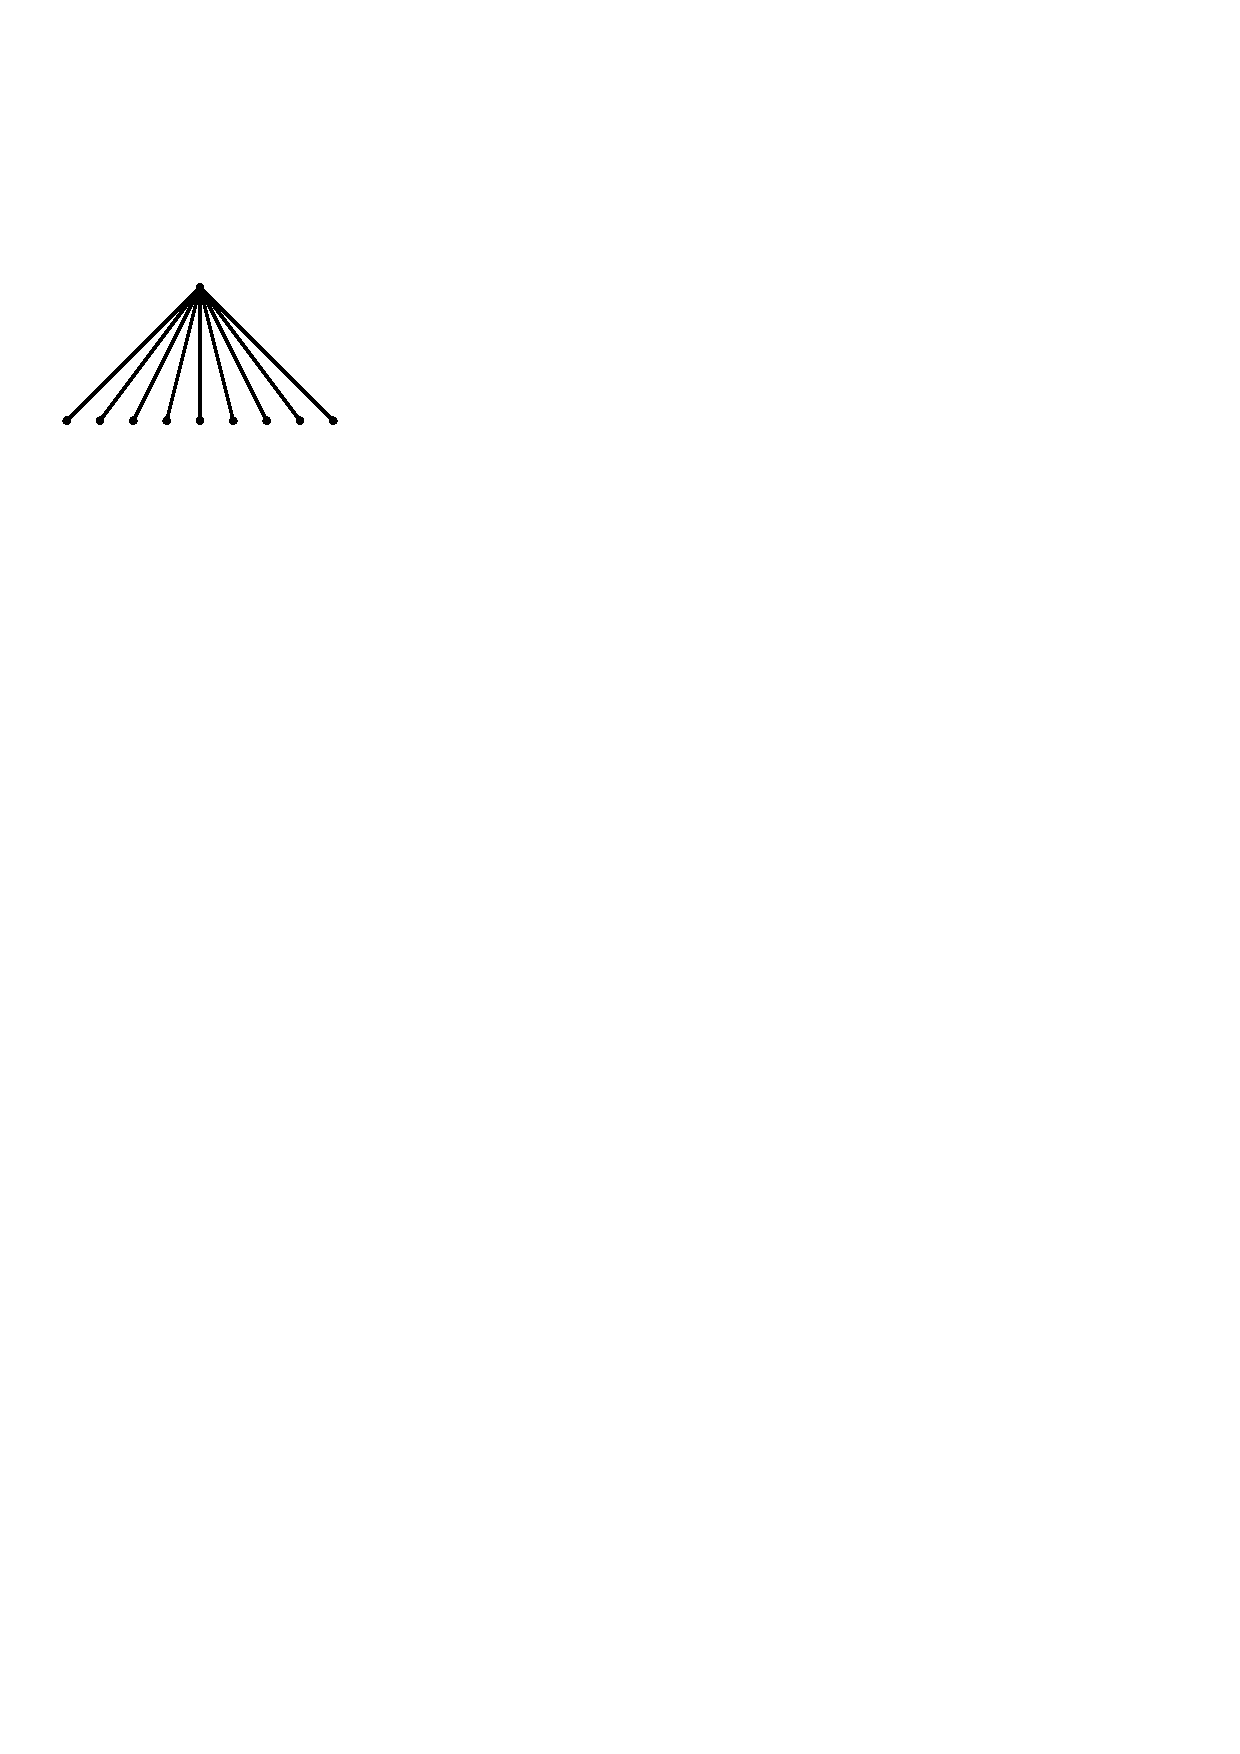
\includegraphics[width=.25\textwidth]{figs/s} & $\CartProd$ & 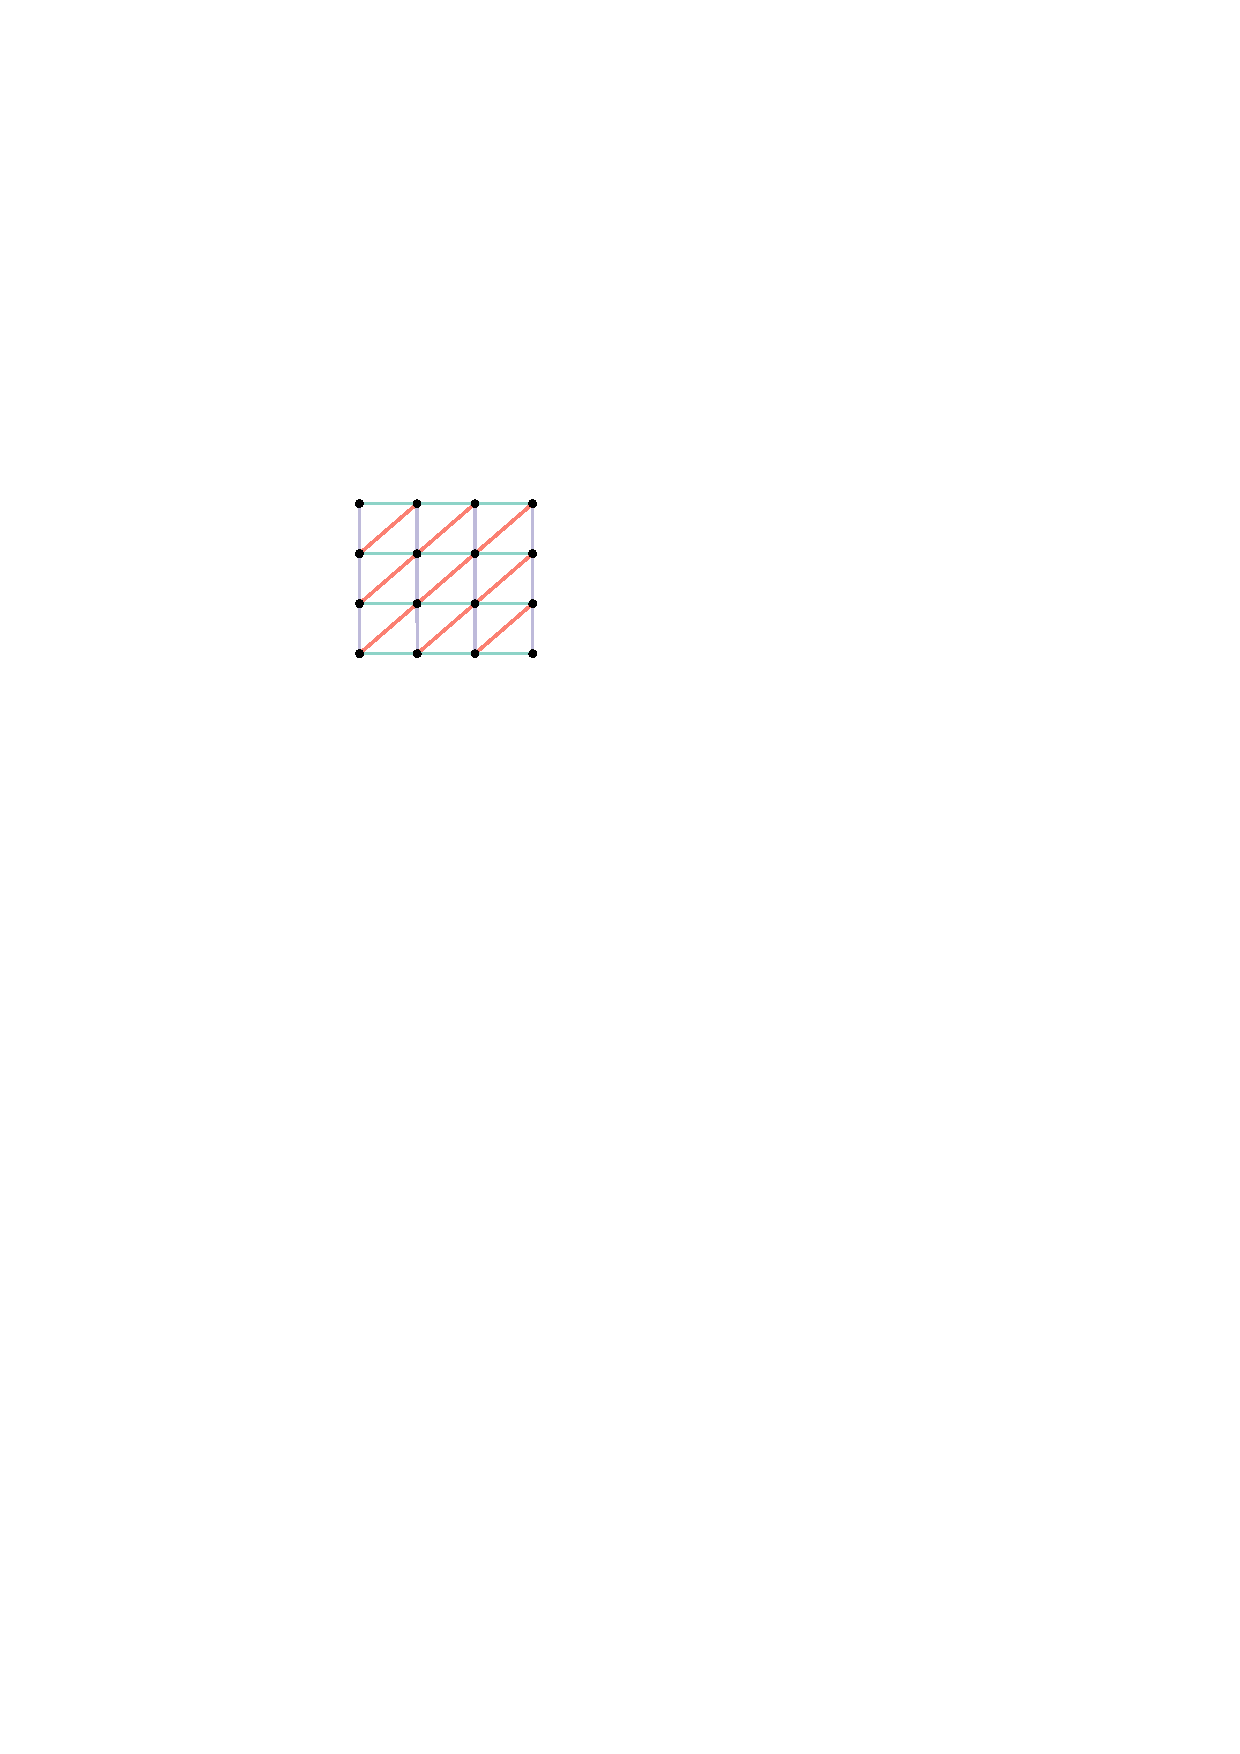
\includegraphics[width=.25\textwidth]{figs/q} & $=$
			& 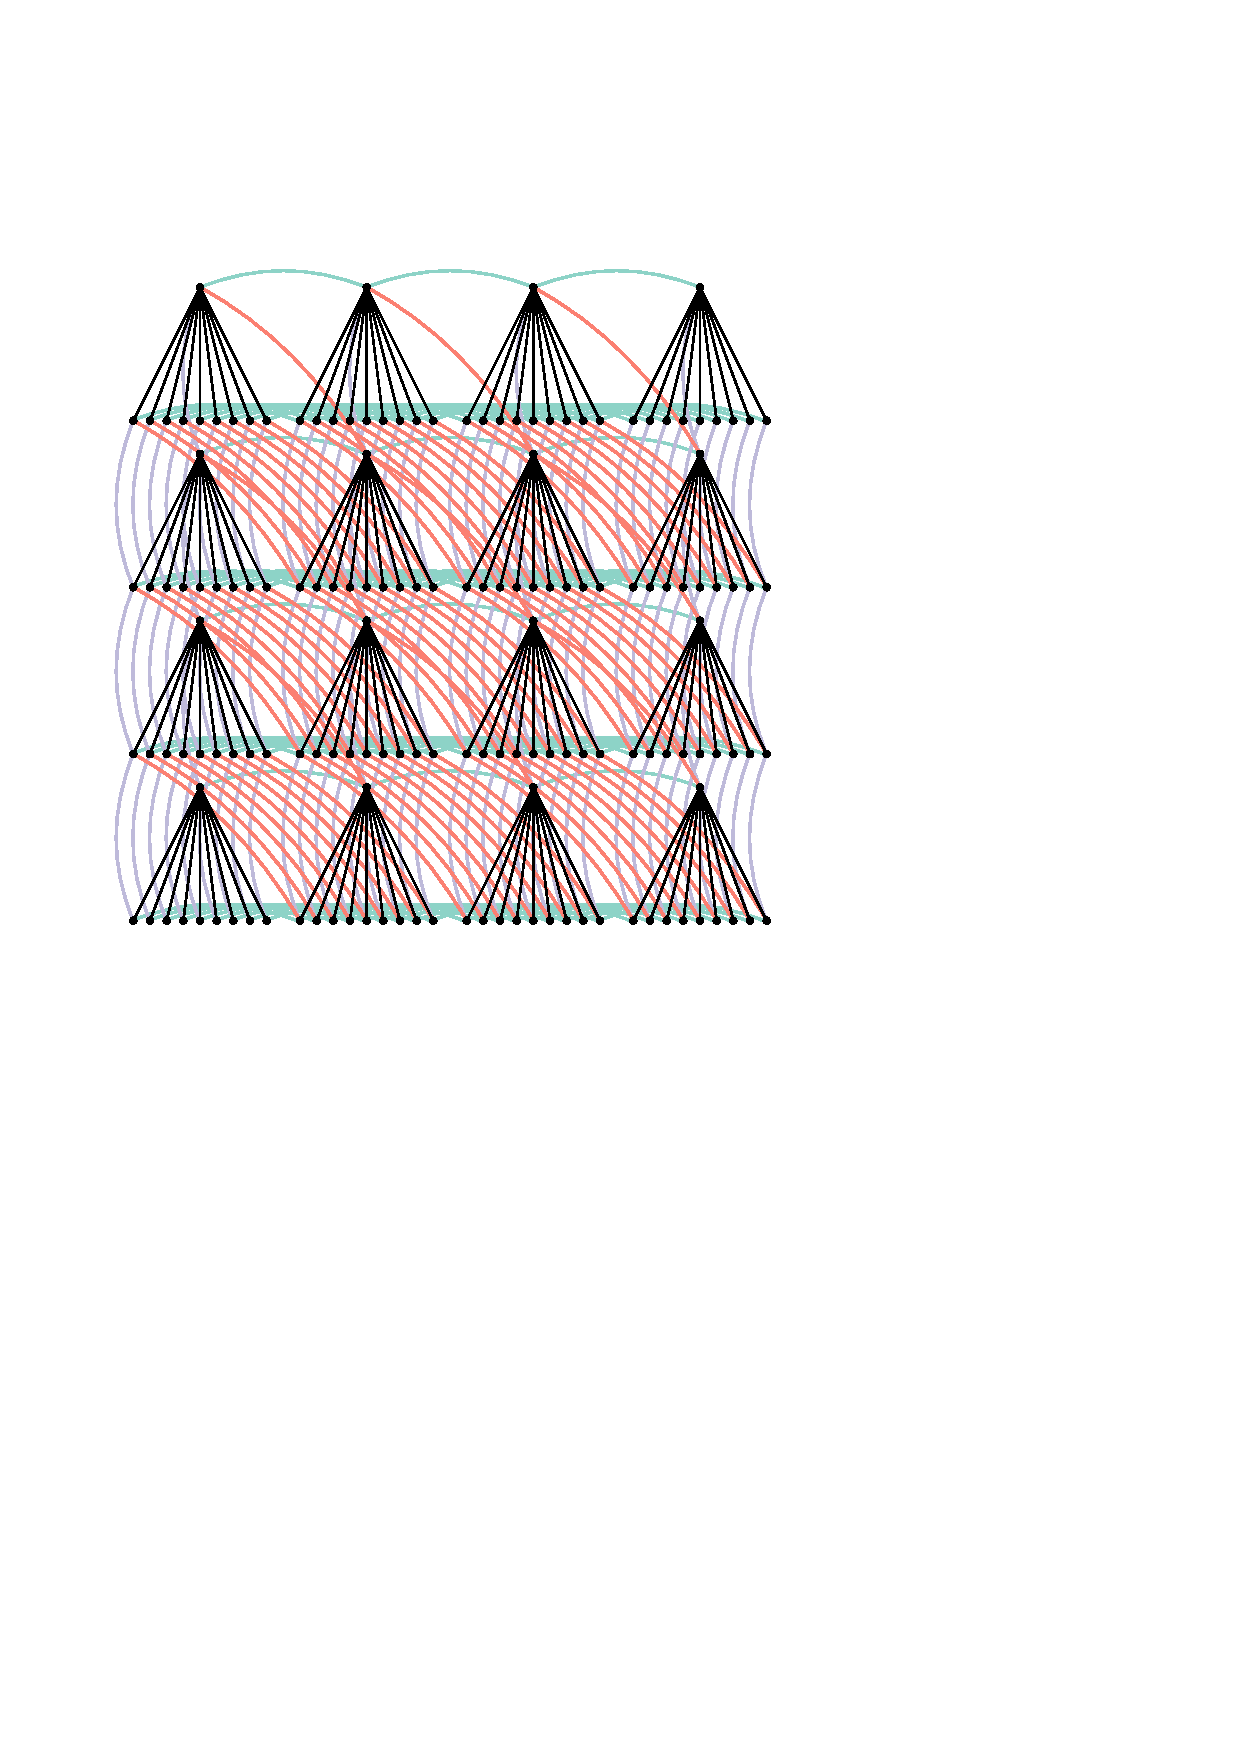
\includegraphics[width=.3\textwidth]{figs/product}
		\end{tabular}
	\end{center}
	% 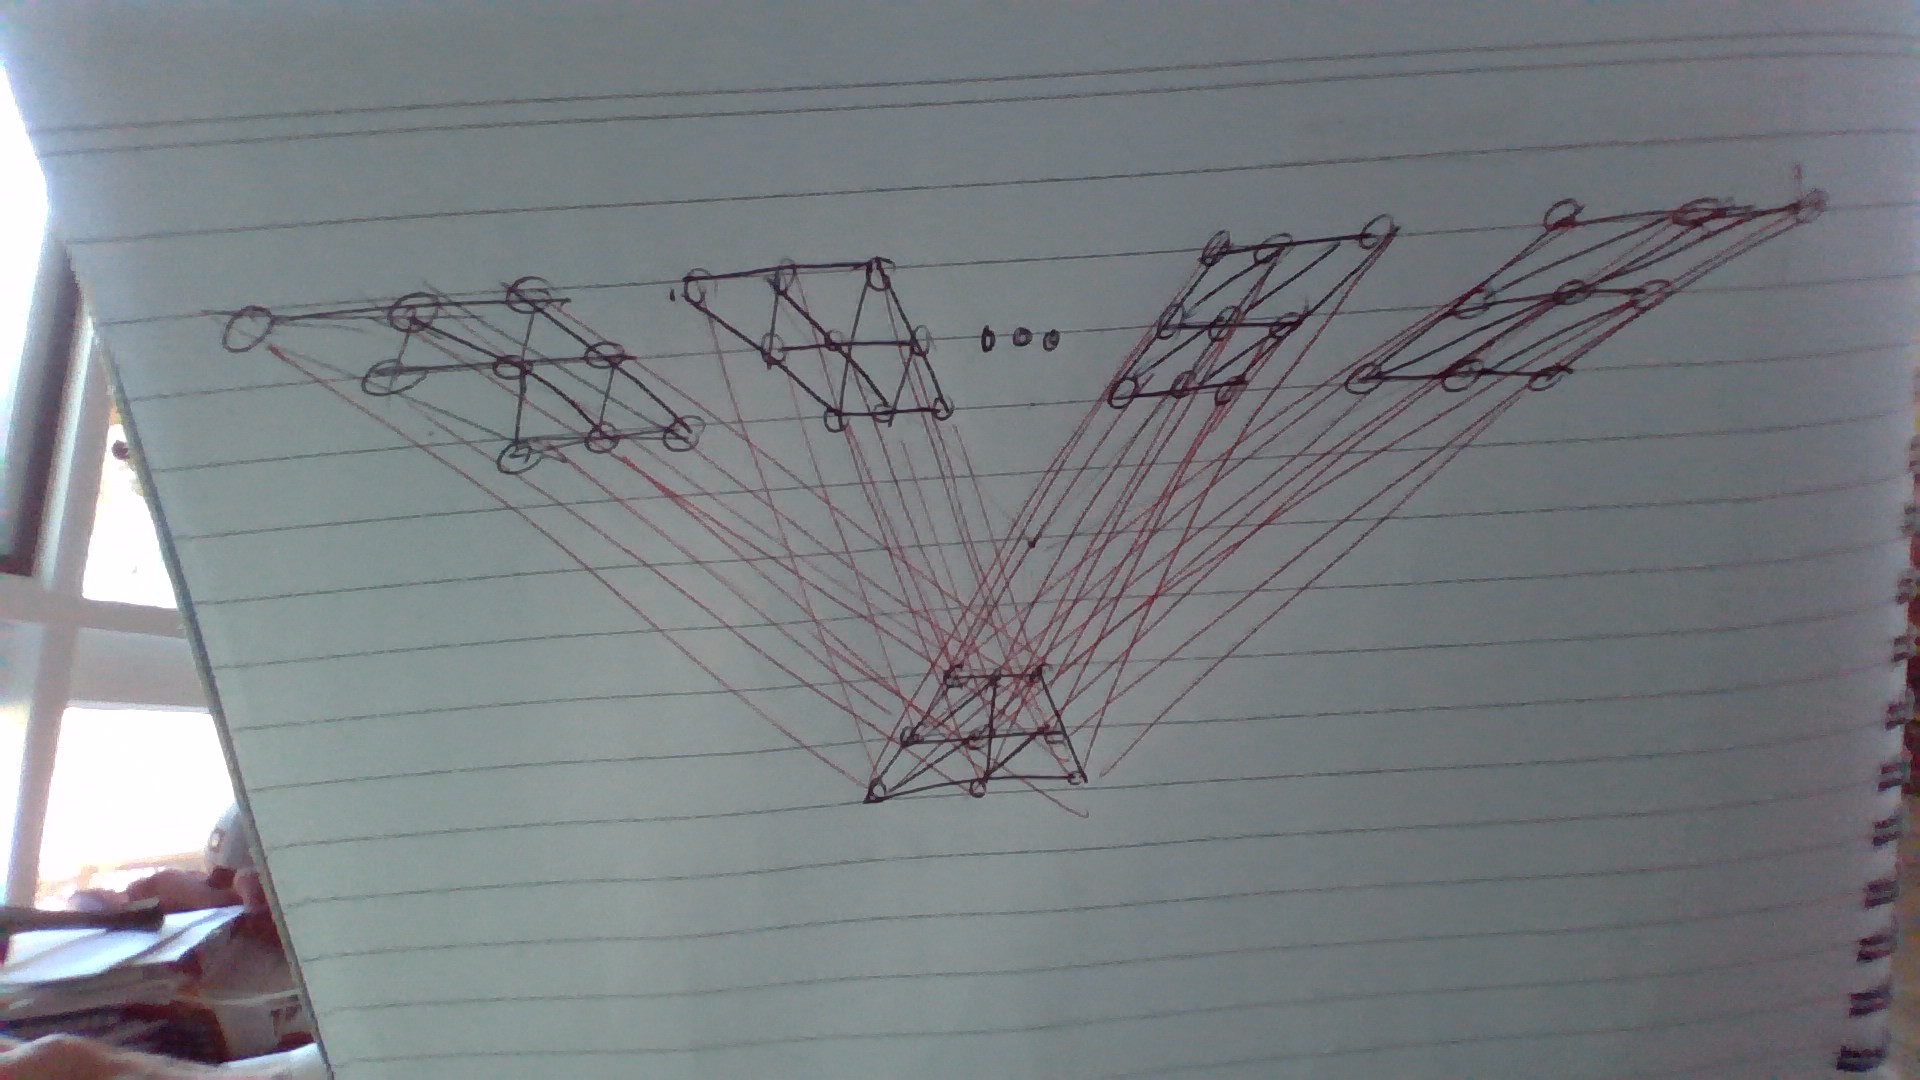
\includegraphics[width=\textwidth]{figs/figure}
	\caption{$S_9 \CartProd H_4$.}
	\label{graph}
\end{figure}


\subsection*{Subdivisions}

A noteworthy consequence of \Cref{family} is that it resolves a conjecture of \citet{BO99}. A graph $G'$ is a \textit{subdivision} of a graph $G$ if $G'$ can be obtained from $G$ by replacing the edges $vw$ of $G$ by internally disjoint paths $P_{vw}$ with endpoints $v$ and $w$. If each $P_{vw}$ has exactly $k$ internal vertices, then $G'$ is the \emph{$k$-subdivision} of $G$. If each $P_{vw}$ has at most $k$ internal vertices, then $G'$ is a \emph{$(\leq k)$-subdivision} of $G$. \citet{BO99} conjectured that the stack-number of $(\leq k)$-subdivisions ($k$ fixed)  is not much less than the stack-number of the original graph. More precisely:

\begin{conj}[\citep{BO99}]
\label{B_conj}
There exists a function $f$ such that for every graph $G$ and integer $k$, if $G'$ is any $(\leq k)$-subdivision of $G$, then $\sn(G) \leq f(\sn(G’),k)$.
\end{conj}

\citet{DujWoo05} established a connection between this conjecture and the question of whether stack-number is bounded by queue-number. In particular, they showed that if
\cref{B_conj} is true, then stack-number is bounded by queue-number. Since \cref{family} shows that stack-number is not bounded by queue-number, \cref{B_conj} is false. The proof of \citet{DujWoo05} is based on the folllowing key lemma: every graph $G$ has a $3$-stack subdivision with $1+2 \ceil{\log_2\qn(G)}$ division vertices per edge. Applying this result to the graph $G=S_b\CartProd H_n$ in \cref{family},
the $5$-subdivision of $S_b\CartProd H_n$ has a $3$-stack layout. If \cref{B_conj} was true, then $\sn(S_b\CartProd H_n) \leq f( 3,5)$, contradicting \cref{family}.

%Specifically,
%\[
%    \mathcal{F} := \{ S_b\square H_n : b,n\in\N\}
%\]
%where $S_b$ denotes the star with $b$ leaves and $H_n$ is the triangulated $n\times n$ grid.

%\todo[inline]{PM: Does anyone know if there is a standard box operator that is typeset like this $S\boxtimes H$ or $S\boxdot H$ instead of like this $S\square H$ or like this $S\Box H$?  I tried square and Box. DW: I defined \texttt{CartProd} which typesets okay $A \CartProd B$	.}


%The graph $G$ in \cref{family} is obtained as follows (See \figref{graph}): Let $S_b$ denote the star graph with root $r$ and $b$ leaves.  For an even positive integer $n$, let $H_n$ be the $n\times n$ triangulated grid, defined by $V(H_n):=\{1,\ldots,n\}^2$ and
%\begin{align*}
%E(H_n) & :=\{(x,y)(x+1,y):x\in\{1,\ldots,n-1\},\,y\in\{1,\ldots,n\}\} \\
%& \qquad \cup \{(x,y)(x,y+1):x\in\{1,\ldots,n\},\,y\in\{1,\ldots,n-1\}\} \\
%& \qquad \cup \{(x,y+1)(x+1,y):x,y\in\{1,\ldots,n-1\}\} \enspace .
%\end{align*}
%We consider the graph $G:=S_b\CartProd H_n$. That is, $V(G)=V(S_b)\times V(H_n)$ where vertices $(v_1,w_1),(v_2,w_2)\in V(G)$ are adjacent whenever $v_1=w_1$ and $v_2w_2\in E(H_n)$, or $v_1w_1\in E(S_b)$ and $v_2=w_2$.


%SAY SOMETHING ABOUT THE RESULTS OF \citet{Pupyrev20}. I EXPECT WE SOLVE SOME OPEN PROBLEM HERE.\todo{PM:Not really, his open problem is about $H\boxtimes P$ where $H$ has bounded treewidth.}

\subsection*{Is Queue-number Bounded by Stack-Number? }

It remains open whether queues are more powerful than stacks; that is, whether queue-number is bounded by stack-number. Several reults are known about this problem. \citet{HLR92} showed that every 1-stack graph has a 2-queue layout. \citet{DJMMUW20} showed that planar graphs have bounded queue-number. (Note that graph products also feature heavily in this proof.)\ Since 2-stack graphs are planar, this implies that 2-stack graphs have bounded queue-number. It is open whether 3-stack graphs have bounded queue-number. In fact, the case of three stacks is as hard as the general question. \citet{DujWoo05} proved that queue-number is bounded by stack-number if and only if 3-stack graphs have bounded queue-number. Moreover, if this is true then stack-number is bounded by a polynomial function of queue-number.


\section{Stack and Queue Layouts of Cartesian Products}

\todo[inline]{Add discussion of result of \citet{BK79}: $\sn(G\CartProd H) \leq \sn(G) + \dsn(H)$ for bipartite $H$. Highlight the key difference between stack and queue layouts is that we need $H$ to be bipartite here.}

\todo{mention results of \citet{Pupyrev20} about bipartite graphs?}

First we prove that $\qn(S_b\CartProd H_n)\leq 4$, as claimed in \cref{family}. We need the following definition due to \citet{Wood-Queue-DMTCS05}. A queue layout $(\varphi,\prec)$ is \emph{strict} if for every vertex $u\in V(G)$ and for all neighbours $v,w\in N_G(u)$, if $u\prec v,w$ or $v,w \prec u$, then $\varphi(uv)\neq \varphi(uw)$. Let $\sqn(G)$ be the minimum integer $k$ such that $G$ has a strict $k$-queue layout. To see that $\sqn(H_n) \leq 3$, order the vertices row-by-row and then left-to-right within a row, with vertical edges in one queue, horizontal edges in one queue, and diagonal edges in another queue.
\citet{Wood-Queue-DMTCS05} proved that $\qn(G\CartProd H) \leq \qn(G) + \sqn(H)$ for all graphs $G$ and $H$. Of course, $S_b$ has a 1-queue layout (since no two edges are nested for any vertex-ordering). Thus $\qn(S_b \CartProd H_n)\leq 4$.

\section{The Main Proof}

We now turn to the proof of our main result, the lower bound on $\sn(G)$, where $G:= S_b\CartProd H_n$. Consider a hypothetical $s$-stack layout $(\varphi,\prec)$ of $G$ where $n$ and $b$ are chosen sufficiently large compared to $s$ as detailed below. We begin with three lemmata that, for sufficiently large $b$, provide a large subgraph $S_d$ of $S_b$ for which the induced stack layout of $S_d\CartProd H_n$ is highly structured.

For each node $v$ of $S_b$, define $\pi_v$ as the permutation of $\{1,\ldots,n\}^2$ in which $(x_1,y_1)$ appears before $(x_2,y_2)$ if and only if $(v,(x_1,y_1))\prec (v,(x_2,y_2))$. The following lemma is an immediate consequence of the Pigeonhole Principle:

\begin{lem}\lemlabel{uniform_order}
    There exists a permutation $\pi$ of $\{1,\ldots,n\}^2$ and a set $L_1$ of leaves of $S_b$ of size $a\ge b/(n^2)!$ such that $\pi_{v}=\pi$ for each $v\in L_1$.
\end{lem}

% \todo[inline]{If we cared, we could improve this to $b/2^{cn^2}$ since we only use the weaker property (P3) in the final proof. DW: I don't care. }

For each leaf $v$ in $L_1$, let $\varphi_v$ be the edge colouring of $H_n$ defined by $\varphi_v(xy):=\varphi((v,x)(v,y))$ for each $xy\in E(H_n)$. Since $H_n$ has maximum degree $6$ and is not 6-regular, it has fewer than $3n^2$ edges.  Therefore there are fewer than $s^{3n^2}$ edge colourings of $H_n$ using $s$ colours.  Another application of the Pigeonhole Principle proves the following:

\begin{lem}\lemlabel{uniform_colour}
    There exists a subset $L_2\subseteq L_1$ of size $c\ge a/s^{3n^2}$
    and an edge colouring $\phi:E(H_n)\to\{1,\ldots,s\}$ such that $\varphi_v=\phi$ for each $v\in L_2$.
\end{lem}


Let $S_{c}$ be the subgraph of $S_b$ induced by $L_2\cup\{r\}$. The preceding two lemmata ensure that, for distinct leaves $v$ and $w$ of $S_{c}$, the stack layouts of the isomorphic graphs $G[\{(v,p):p\in V(H_n)\}]$ and $G[\{(w,p):p\in V(H_n)\}]$ are identical. The next lemma is a statement about the relationships between the stack layouts of $G[\{(v,p):v\in V(S_{c})\}]$ and $G[\{(v,q):v\in V(S_{c})\}]$ for  distinct $p,q\in V(H_n)$.  It does not assert that these two layouts are identical but it does state that they fall into one of two categories.

\begin{lem}\lemlabel{forward_or_backward}
    There exists a sequence $L_3:=u_1,\ldots,u_{d}$ with $\{u_1,\ldots,u_{d}\}\subseteq L_2$ of length $d\ge c^{1/2^{n^2-1}}$ such that, for each $p\in V(H_n)$, either  $(u_1,p)\prec (u_2,p)\prec\cdots\prec (u_{d},p)$ or $(u_1,p)\succ (u_2,p)\succ\cdots\succ (u_{d},p)$.
\end{lem}

\begin{proof}
    Let $p_1,\ldots,p_{n^2}$ denote the vertices of $H_n$ in any order.
    Begin with the sequence $S_1:=v_{1,1},\ldots,v_{1,c}$ that contains all $c$ elements of $L_2$ ordered so that $(v_{1,1},p_1)\prec\cdots\prec(v_{1,c},p_1)$.  For each $i\in\{2,\ldots,n^2\}$, the Erd\H{o}s-Szekeres Theorem~\citep{ES35} implies that $S_{i-1}$ contains a subsequence $S_i:=v_{i,1},\ldots,v_{i,|S_i|}$ of length $|S_i|\ge \sqrt{|S_{i-1}|}$ such that $(v_{i,1},p_i)\prec\cdots\prec(v_{i,|S_i|},p_i)$ or $(v_{i,1},p_i)\succ\cdots\succ(v_{i,|S_i|},p_i)$.  It is straightforward to verify by induction on $i$ that $|S_i| \ge c^{1/2^{i-1}}$ resulting in a final sequence $S_{n^2}=:L_3$ of length at least $c^{1/2^{n^2-1}}$.
\end{proof}

For the rest of the proof we will work with the star $S_d$ whose leaves are $u_1,\ldots,u_d$ described in \lemref{forward_or_backward}.  Consider the (improper) vertex colouring of $H_n$ obtained by colouring each vertex $p\in V(H_n)$ \emph{red} if $(u_1,p)\prec\cdots\prec (u_d,p)$ and colouring $p$ \emph{blue} if $(u_1,p)\succ\cdots\succ(u_d,p)$. We need the following famous Hex Lemma~\citep{Gale79}.

\begin{lem}[\citep{Gale79}] \label{hex_lemma}
Every red--blue vertex colouring of the graph $H_n$	contains an $n$-vertex path $R$ consisting entirely of red vertices or entirely of blue vertices.
\end{lem}

%\begin{proof}
%    The dual of $H_n$ is the board on which the game Hex is played.  The well-known \emph{Hex Lemma} states that any colouring of the vertices of $H_n$ with colours red and blue contains exactly one of the following \cite{Gale79}:
%    \begin{compactenum}
%        \item a path with endpoints $(x,1)$ and $(x',n)$ consisting entirely of red vertices, for some $x,x'\in\{1,\ldots,n\}$; or
%        \item a path with endpoints $(1,y)$ and $(n,y')$ consisting entirely of blue vertices, for some $y,y'\in\{1,\ldots,n\}$.
%    \end{compactenum}
%    In either case, the path contains at least $n$ vertices and therefore has a $n$-vertex subpath consisting entirely of red vertices or entirely of blue vertices.
%\end{proof}

Without loss of generality, assume that the path $R:=p_1,\ldots,p_n$ defined by \cref{hex_lemma} (with the above-defined colouring) consists entirely of red vertices, so that $(u_1,p_j)\prec\cdots\prec (u_d,p_j)$ for each $j\in\{1,\ldots,n\}$.  Recall that $(\varphi,\prec)$ is a hypothetical $s$-stack layout of $G$ and therefore it is also an $s$-stack layout of the subgraph $X:=S_d\CartProd R$. In particular, there is no set of greater than $s$ pairwise crossing edges in $X$. The following result finishes the proof by showing that such a set exists when $n> 2s$ and $d\ge (s+1)2^{n}$ (which is implied if $n=2s+1$ and $b \ge (n^2)!\, s^{3n^2}\, ((s+1)2^n)^{2^{n^2-1}} $).


\begin{lem}\lemlabel{twister}
    The graph $X$ contains a set of edges of size at least $\min\{\lfloor d/2^{n}\rfloor,\lceil n/2\rceil\}$ that are pairwise crossing with respect to $\prec$.
\end{lem}

\begin{proof}
	Extend the total order $\prec$ onto a partial order over subsets of $V(G)$ so that, for $V,W\subseteq V(G)$,  $V\prec W$ if and only if $v\prec w$ for each $v\in V$ and each $w\in W$.  We abuse notation slightly by using $\prec$ to compare elements of $V(G)$ and subsets of $V(G)$ so that, for $v\in V(G)$ and $V\subseteq V(G)$, $v\prec V$ denotes $\{v\}\prec V$.
    We will define sets $A_1\supseteq \cdots\supseteq A_{n}$ of leaves of $S_d$ so that each $A_i$ satisifies the following conditions:
    \begin{compactenum}[(C1)]
        \item $A_i$ contains $d_i\ge d/2^{i-1}$ leaves of $S_d$.
        \item Each leaf $v\in A_i$ defines an $i$-element vertex set $Z_{i,v}:=\{(v,p_j):j\in\{1,\ldots,i\}\}$.  For any distinct $v,w\in A_i$, the sets $Z_{i,v}$ and $Z_{i,w}$ are \emph{separated} with respect to $\prec$; that is, $Z_{i,v}\prec Z_{i,w}$ or $Z_{i,v}\succ Z_{i,w}$.
    \end{compactenum}

    Before defining $A_1,\ldots,A_n$ we first show how the existence of the set $A_n$ implies the lemma.  To avoid triple-subscripts, let $d':=d_n\ge d/2^{n-1}$.   The set $A_n$ defines vertex sets $Z_{n,v_1}\prec\cdots\prec Z_{n,v_{d'}}$.  Refer to \figref{twister}. Recall that $r$ is the root of $S_b$ so it is adjacent to each of $v_{1},\ldots,v_{d'}$ in $S_d$.  Therefore, for each $j\in\{1,\ldots,n\}$ and each $i\in\{1,\ldots,d'\}$, the edge $(r,p_j)(v_i,p_j)$ is in $X$. Therefore, $(r,p_j)$ is adjacent to an element of each of $Z_{n,v_1},\ldots,Z_{n,v_{d'}}$.
	\begin{figure}
		\begin{center}
			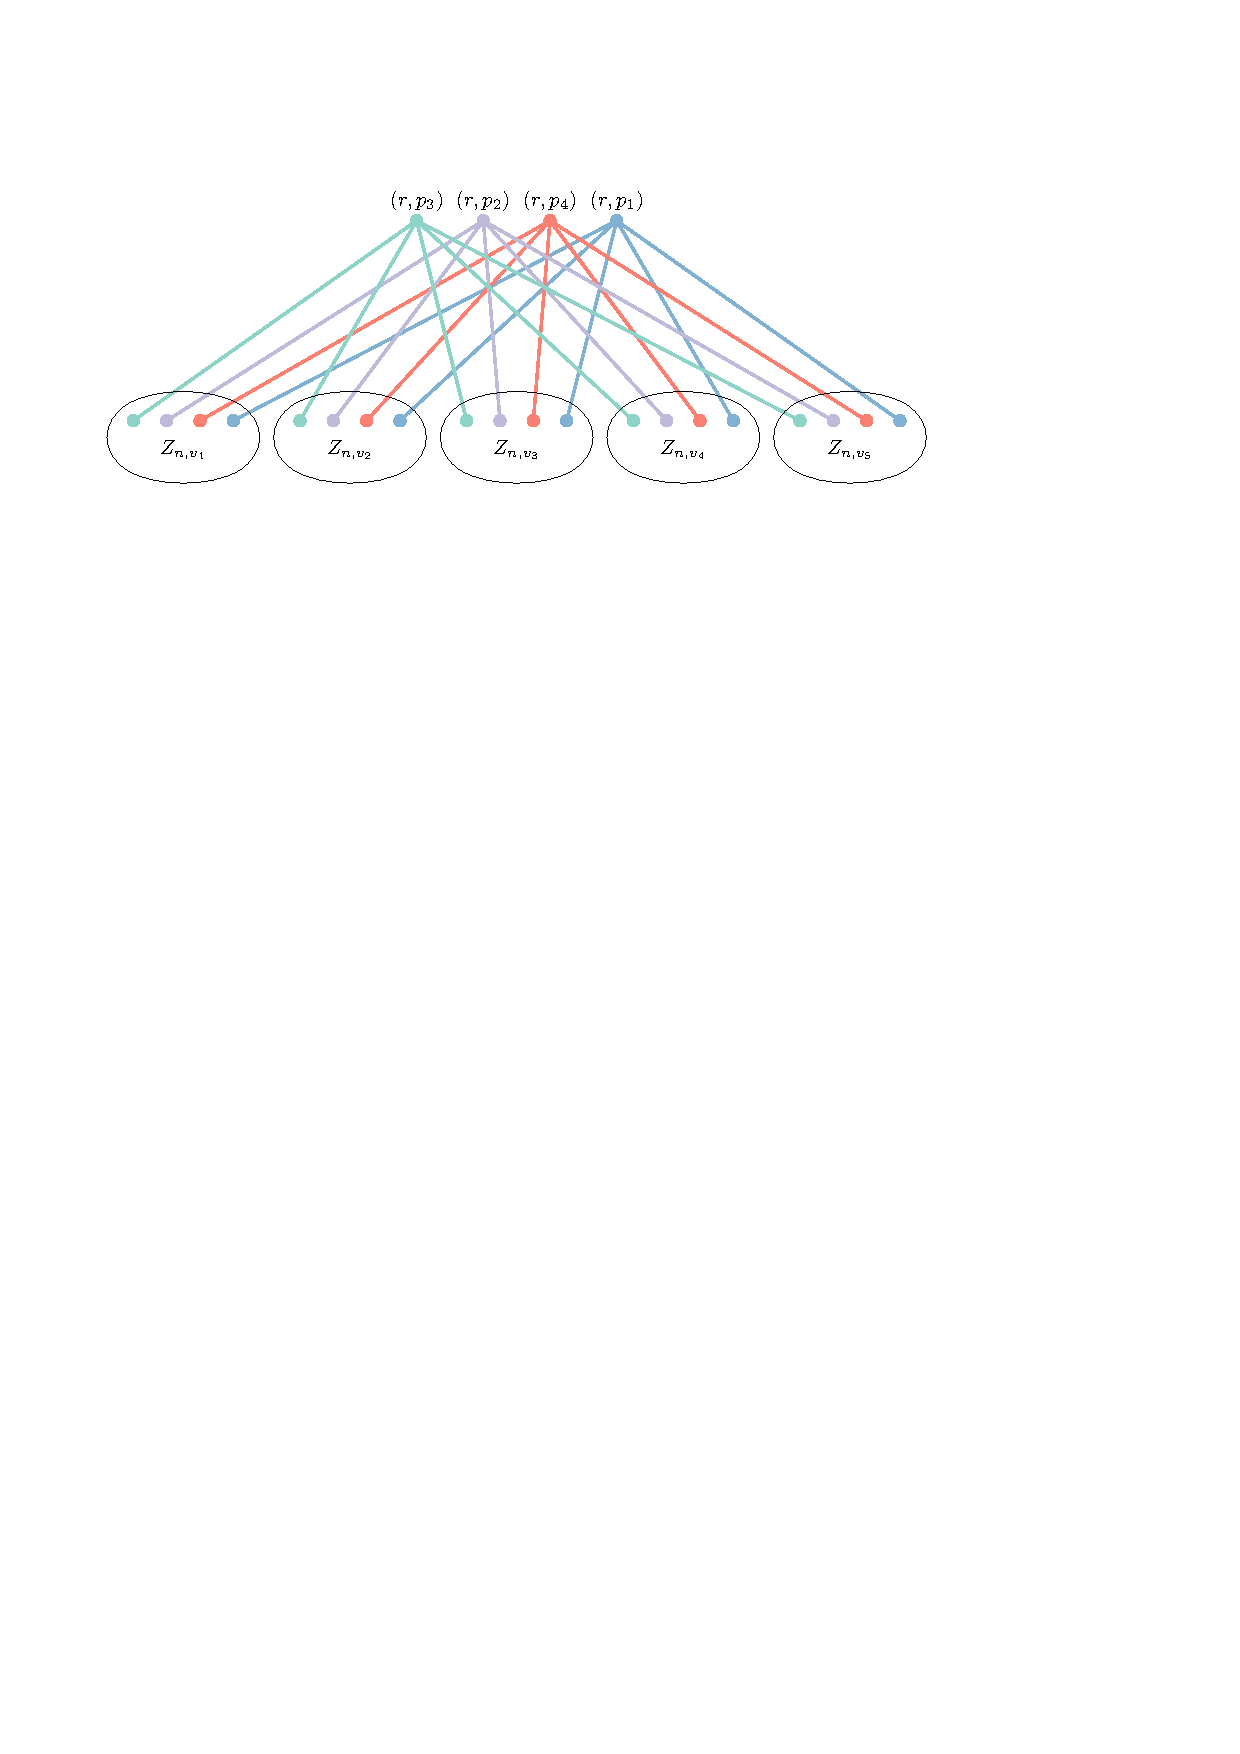
\includegraphics{figs/twister}
		\end{center}
		\caption{The sets $Z_{n,v_1},\ldots,Z_{n,v_{d'}}$ ($n=4$, $d'=5$).}
		\figlabel{twister}
	\end{figure}

    Since $Z_{n,v_1},\ldots,Z_{n,v_{d'}}$ are separated with respect to $\prec$, when viewed from afar, this situation looks like a complete bipartite graph $K_{n,d'}$ with the root vertices $L:=\{(r,p_j):j\in\{1,\ldots,n\}\}$ in one part and the groups $R:=Z_{n,v_1}\cup\cdots\cup Z_{n,v_{d'}}$ in the other part.  Any linear ordering of $K_{n,d'}$ has a large set of pairwise crossing edges so, intuitively, the induced subgraph $X[L\cup R]$ should also have a large set of pairwise crossing edges. We can formalize this as follows: Label the vertices in $L$ as $r_1,\ldots,r_n$ so that $r_1\prec \cdots\prec r_{n}$.  Then at least one of the following two cases applies (see \figref{median}):
    \begin{enumerate}
        \item $Z_{n,\lfloor d'/2\rfloor}\prec r_{\lceil n/2\rceil}$ in which case the graph between $r_{\lceil n/2\rceil},\ldots,r_{n}$ and $Z_{n,1},\ldots,Z_{n,\lfloor d'/2\rfloor}$ has a set of at least $\min\{\lfloor d'/2\rfloor,\lceil n/2\rceil\}$ pairwise-crossing edges.
        \item $r_{\lceil n/2\rceil}\prec Z_{\lceil d'/2\rceil+1}$ in which case the graph between $r_1,\ldots,r_{\lceil n/2\rceil}$ and $Z_{\lceil d'/2\rceil+1},\ldots,Z_{d'}$ has a set of $\min\{\lfloor d'/2\rfloor,\lceil n/2\rceil\}$ pairwise-crossing edges.
    \end{enumerate}
	\begin{figure}
		\begin{center}
			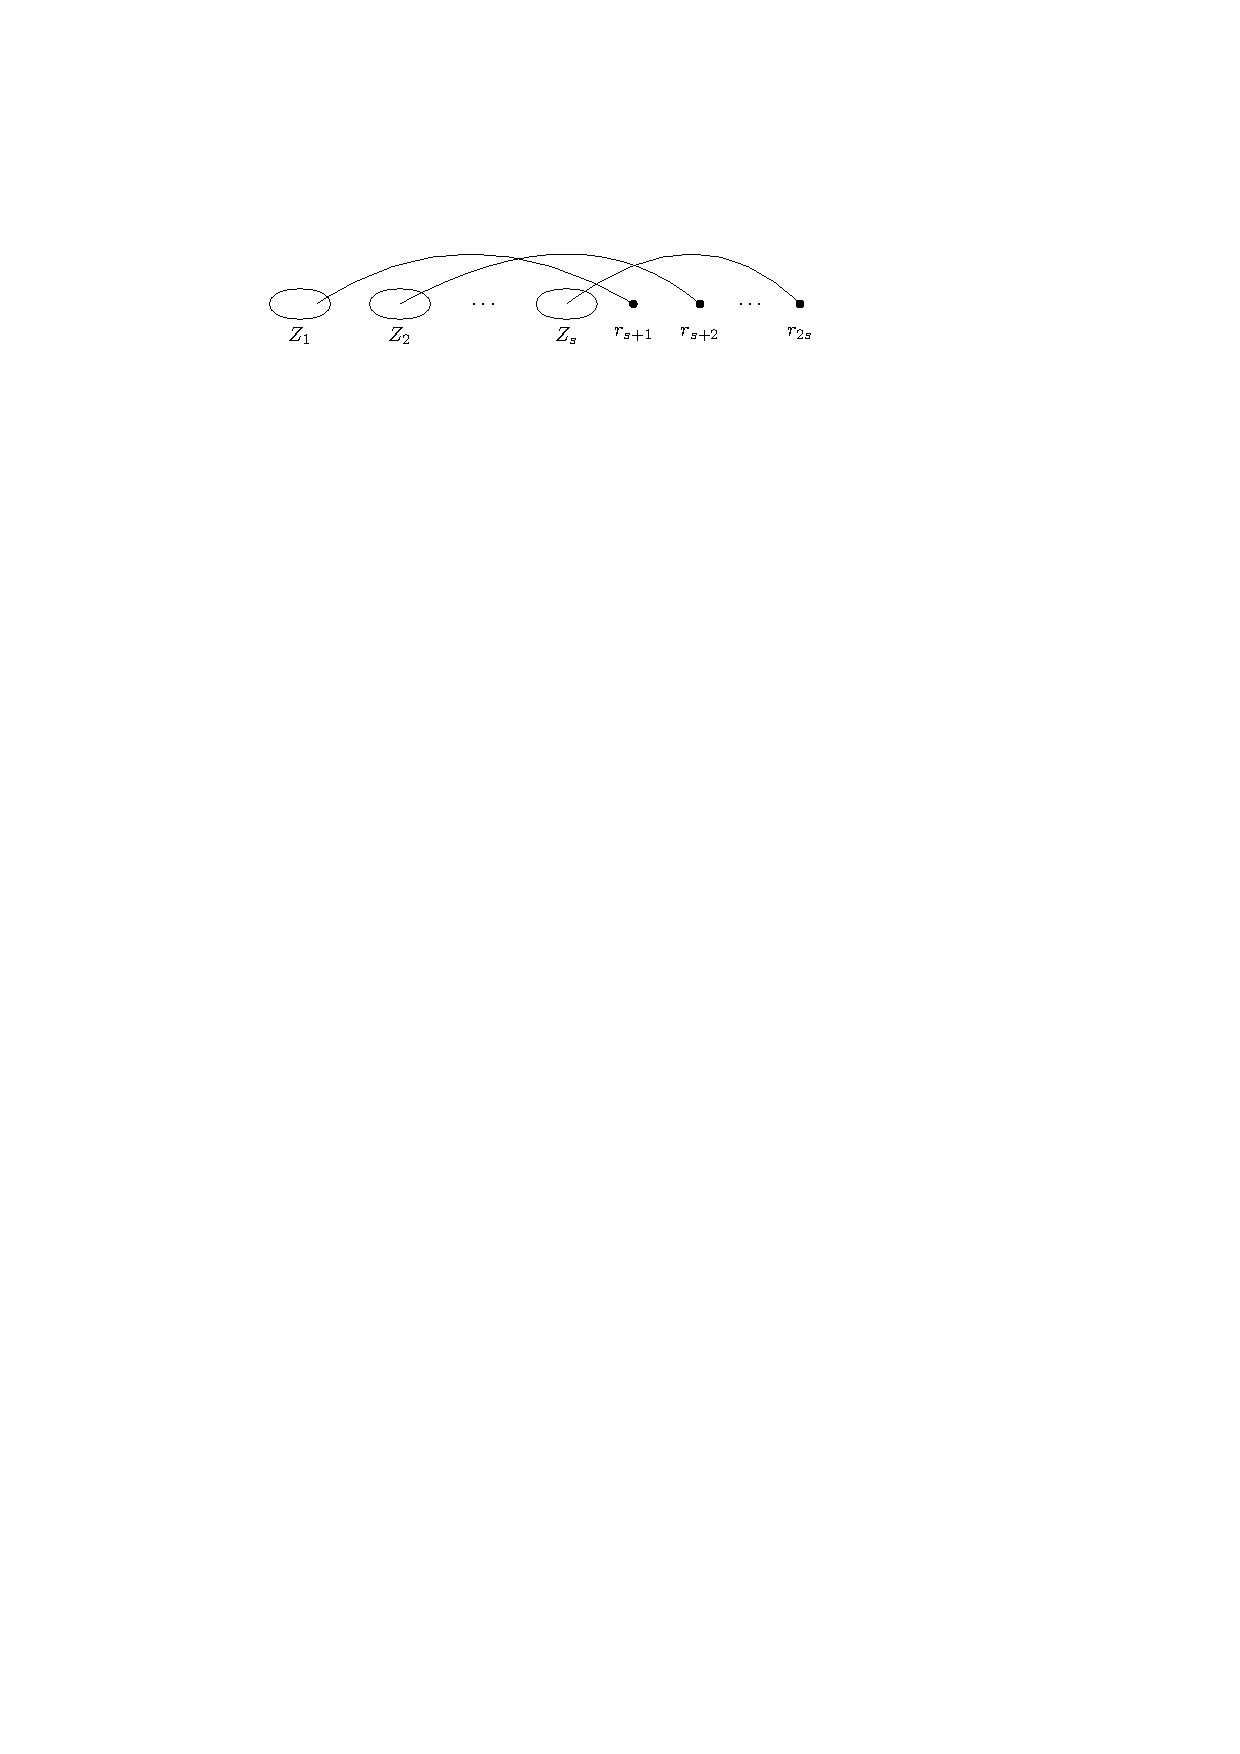
\includegraphics{figs/median-1} \\ 1 \\[2em]
			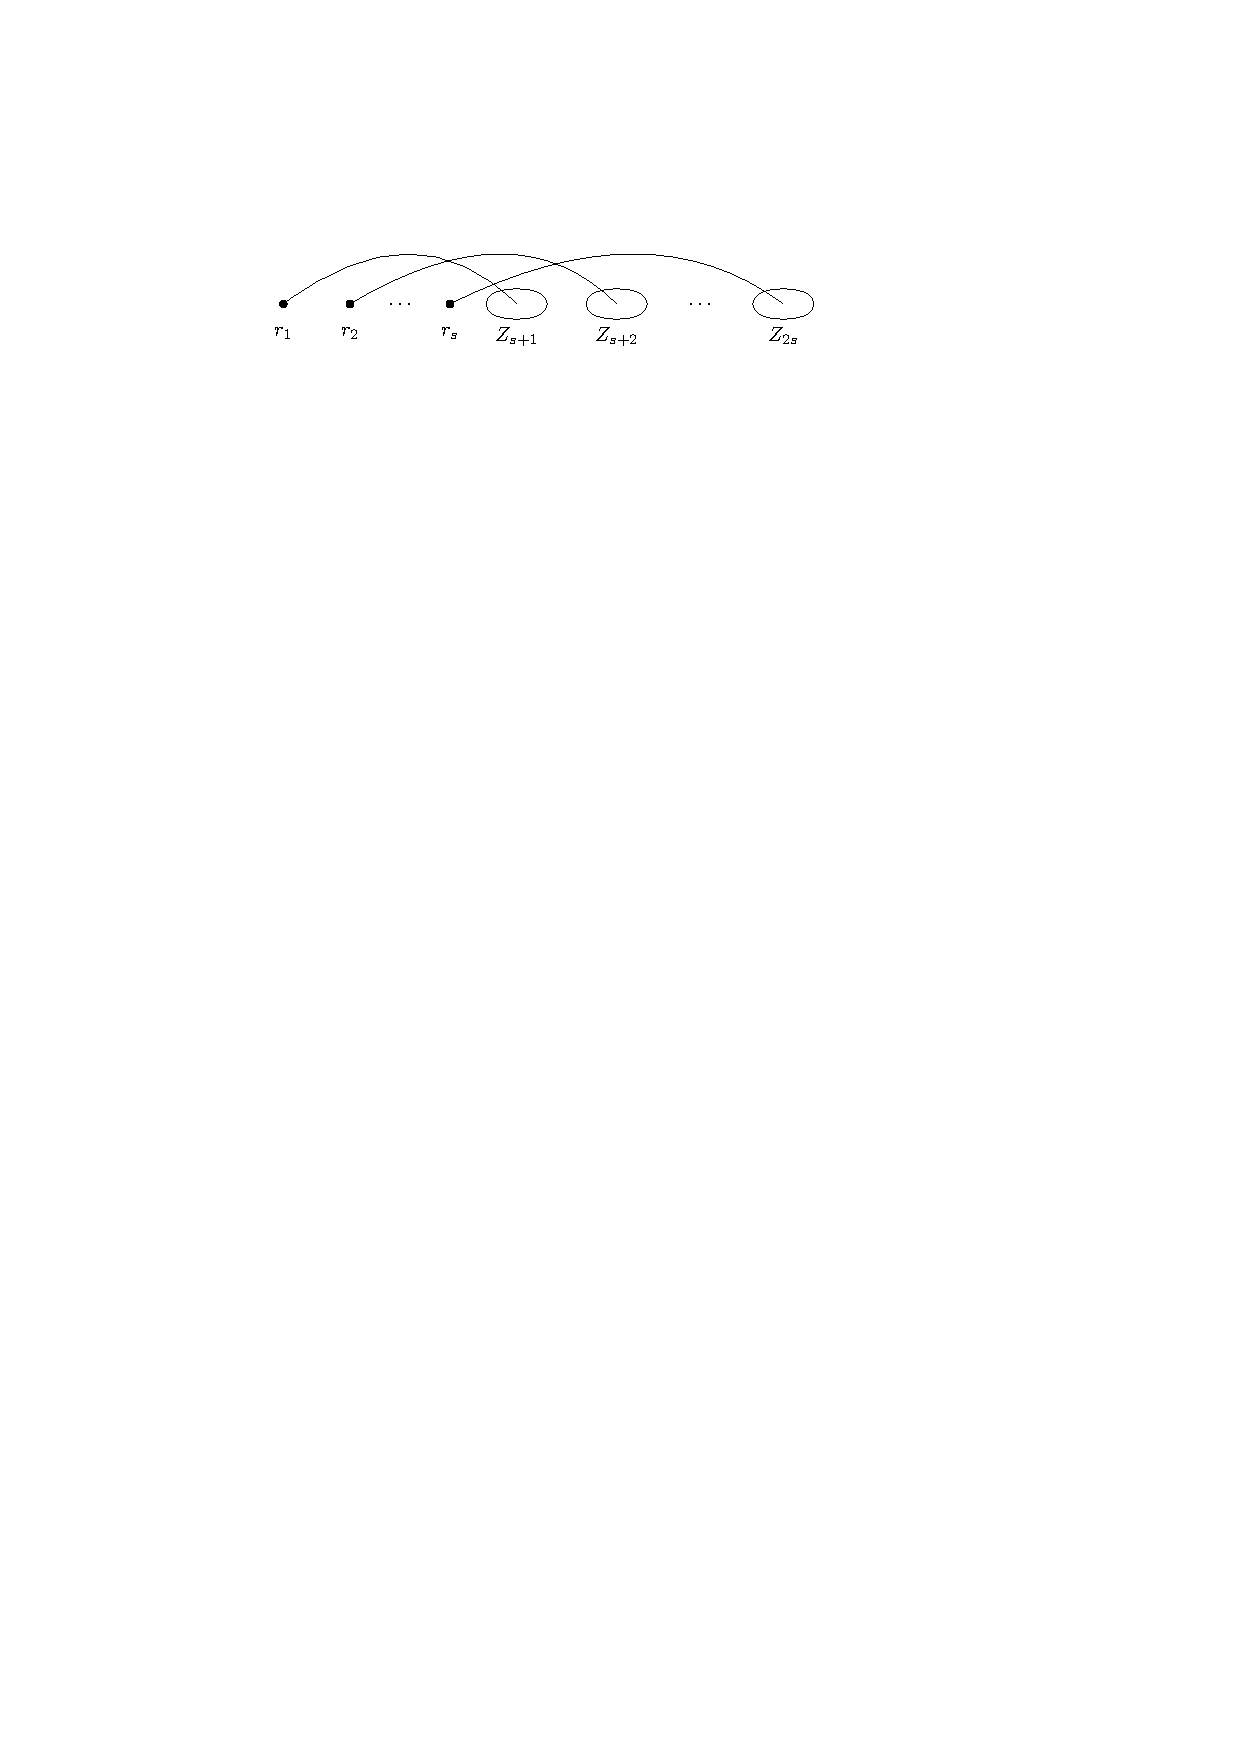
\includegraphics{figs/median-2} \\ 2
		\end{center}
		\caption{The two cases in the proof of \lemref{twister}.}
		\figlabel{median}
	\end{figure}
	Since, by (C1), $d'\ge d/2^{n-1}$, either case results in a set of pairwise-crossing edges of size at least $\min\{\lfloor d/2^n\rfloor,\lceil n/2\rceil\}$, as claimed.

    All that remains is to define the sets $A_1\supseteq\cdots\supseteq A_n$ that satisfy (C1) and (C2).  Let $A_1$ be the set of all the leaves of $S_d$.  For each $i\in\{2,\ldots,n\}$, the set $A_i$ is defined as follows:  Let $Z_1,\ldots,Z_{|A_{i-1}|}$ denote the sets $Z_{i-1, v}$ for each $v\in A_{i-1}$ ordered so that $Z_1\prec\cdots\prec Z_{|A_{i-1}|}$. By Property (C2), this is always possible.	Label the vertices of $A_{i-1}$ as $v_1,\ldots,v_{|A_{i-1}|}$ so that $(v_1,p_{i-1})\prec\cdots\prec (v_r,p_{i-1})$.   (This is equivalent to naming them so that $(v_j,p_{i-1})\in Z_j$ for each $j\in\{1,\ldots,|A_{i-1}|\}$.)  Define the set $A_i:=\{v_{2k+1}:k\in\{0,\ldots,\lfloor(|A_{i-1}|-1)/2\rfloor\}\}=\{v_{j}\in A_{i-1}:\text{$j$ is odd}\}$.  This completes the definition of $A_1,\ldots,A_n$.

	All that remains is to verify that $A_i$ satisfies (C1) and (C2) for each $i\in\{1,\ldots,n\}$.  We do this by induction on $i$. The base case $i=1$ is trivial so we assume from this point on that $i\in\{2,\ldots,n\}$.   To see that $A_i$ satisfies (C1) just observe that $|A_i|=\lceil |A_{i-1}|/2\rceil \ge |A_{i-1}|/2\ge d/2^{i-1}$, where the final inequality follows by applying the inductive hypothesis $|A_{i-1}|\ge d/2^{i-2}$.  Now all that remains is to show that $A_i$ satisfies (C2).

    Recall that, for each $v\in A_{i-1}$, the edge $e_v:=(v,p_{i-1})(v,p_i)$ is in $X$.  We have the following properties:
    \begin{compactenum}[(P1)]
        \item By \lemref{uniform_colour}, $\varphi(e_v)=\phi(p_{i-1}p_i)$ for each $v\in A_{i-1}$.
        \item Since $p_{i-1}$ and $p_i$ are both red, $(v,p_{i-1})\prec (w,p_{i-1})$ if and only if $(v,p_{i})\prec (w,p_{i})$ for each $v,w\in A_{i-1}$.
        \item By \lemref{uniform_order}, $(v,p_{i-1})\prec (v,p_i)$ for every $v\in A_{i-1}$ or $(v,p_{i-1})\succ (v,p_i)$ for every $v\in A_{i-1}$.
    \end{compactenum}
    We claim that these three conditions imply that the vertex sets $\{(v,p_{i-1}):v\in A_{i-1}\}$ and $\{(v,p_i):v\in A_{i-1}\}$ interleave perfectly with respect to $\prec$. More precisely:
	\begin{clm}\clmlabel{interleave} $(v_1,p_{i-1+t})\prec (v_1,p_{i-t}) \prec (v_2,p_{i-1+t}) \prec (v_2,p_{i-t}) \cdots \prec (v_r,p_{i-1+t}) \prec (v_r,p_{i-t})$ for some $t\in\{0,1\}$.
	\end{clm}
	\begin{proof}[Proof of \clmref{interleave}]
		By (P3) we may assume, without loss of generality, that $(v,p_{i-1})\prec (v,p_i)$ for each $v\in A_{i-1}$, in which case we are trying to prove the claim for $t=0$.  Therefore, it is sufficient to show that $(v_j,p_i)\prec (v_{j+1},p_{i-1})$ for each $j\in\{1,\ldots,r-1\}$.  For the sake of contradiction, suppose $(v_j,p_{i})\succ (v_{j+1},p_{i-1})$ for some $j\in\{1,\ldots,r-1\}$. By the labelling of $A_{i-1}$,  $(v_j,p_{i-1})\prec (v_{j+1},p_{i-1})$ so, by (P2),  $(v_{j},p_i) \prec (v_{j+1},p_i)$.  Therefore
		\[
			(v_j,p_{i-1})\prec (v_{j+1},p_{i-1})\prec(v_{j},p_i) \prec
		   (v_{j+1}, p_i) \enspace .
	   	\]
		Therefore the edges $e_{v_j}=(v_j,p_{i-1})(v_j,p_{i})$ and $e_{v_{j+1}}=(v_{j+1},p_{i-1})(v_{j+1},p_i)$ cross with respect to $\prec$.  But this is a contradiction since, by (P1),  $\varphi(e_{v_j}) =\varphi(e_{v_{j+1}})=\phi(p_{i-1}p_i)$.
		This contradiction completes the proof of \clmref{interleave}.
	\end{proof}

% \todo{DW: Why are these $\prec$'s red?  PM: Just me keeping track of which one was the assumption, they don't need to be red.}

We now complete the proof that $A_i$ satisfies (C2). Apply \clmref{interleave} and assume without loss of generality that $t=0$, so that
	\[
		(v_1,p_{i-1})\prec (v_1,p_{i}) \prec (v_2,p_{i-1}) \prec (v_2,p_{i}) \cdots \prec (v_r,p_{i-1}) \prec (v_r,p_{i}) \enspace .
	\]

    For each $j\in\{1,\ldots,r-2\}$, we have $(v_{j+1},p_{i-1})\in Z_{j+1}\prec Z_{j+2}$, so  $(v_j,p_i)\prec (v_{j+1},p_{i-1}) \prec Z_{j+2}$.  Therefore $Z_j\cup\{(v_j,p_i)\} \prec Z_{j+2}$.  By a symmetric argument, $Z_j\cup\{(v_j,p_i)\} \succ Z_{j-2}$ for each  $j\in\{3,\ldots,r\}$.  Finally, since $(v_{j},p_i)\prec (v_{j+2},p_i)$ for each odd $i\in\{1,\ldots,r\}$, we have $Z_{j}\cup\{(v_j,p_i)\} \prec Z_{j+2}\cup\{(v_{j+2},p_i)\}$ for each odd $j\in\{1,\ldots,r-2\}$.  Thus $A_i$ satisifies (C2) since the sets $Z_1\cup\{(v_1,p_i)\},Z_3\cup\{(v_3,p_i)\},\ldots,Z_{2\lfloor (r-1)/2\rfloor+1} \cup (v_{2\lfloor (r-1)/2\rfloor+1},p_i)$ are precisely the sets $Z_{i,1},\ldots,Z_{i,d_i}$ determined by our choice of $A_i$.
\end{proof}

% \begin{lem}\lemlabel{twister}
%     Let $G$ be any graph, let $\prec$ be any linear ordering of $V(G)$,  let $Z_{1}\prec\cdots\prec Z_{2s}$ be subsets of $V(G)$, and let $r_1\prec\cdots\prec r_{2s}$ be vertices of $G$ such that, for each $i,j\in\{1,\ldots,2s\}$, $G$ contains an edge $r_iz_j$ with $z_j\in Z_j$. Then $G$ contains a set of $s$ edges that are pairwise crossing with respect to $\prec$. \todo[inline]{I think we should not re-use $s$ in this lemma. More importantly, do we really need Lemma 6? It could be easily merged into the proof of Lemma 5 where Lemma 6 is used, and this would avoid having to translate notation. It took me a while to realise that $r_1,\dots,r_{2s}$ corresponds to $L$ in Lemma 5.}
% \end{lem}
%
% \begin{proof}
% \end{proof}
%
\section{Open Problems}

Recall that every 1-queue graph has a 2-stack layout \citep{HLR92} and we proved that there are 4-queue graphs with unbounded stack-number. The following questions remain open: Do 2-queue graphs have bounded stack-number? Do 3-queue graphs have bounded stack-number?

Given the role of cartesian products in our proof, it is natural to ask when is $\sn(G_1\CartProd G_2)$ bounded? Note that $H_n$ is a subgraph of a planar Hamiltonian graph (namely, $H_{2n}$), so $\sn(H_n) \leq 2$. So $\sn(G_1\CartProd G_2)$ can be unbounded even when $G_1$ is a star and $\sn(G_2)\leq 2$.
Since $\sn(G_2)\leq 1$ if and only if $G_2$ is outerplanar, the following question naturally arises: Is $\sn(S \CartProd H)$ bounded for every star $S$ and outerplanar graph $H$ with bounded degree? Is $\sn(T \CartProd H)$ bounded for every tree $T$ and outerplanar graph $H$ with bounded degree? The assumption that $H$ has bounded degree is needed since $S_n \CartProd S_n$ contain the 1-subdivision of $K_{n,n}$, which has unbounded stack-number~\citep{Blankenship-PhD03}.

Since $H_n\subseteq P \boxtimes P$\todo{$\boxtimes$ is not defined} where $P$ is the $n$-vertex path, \cref{family} implies that $\sn(S\boxtimes P\boxtimes P)$ is unbounded for stars $S$ and paths $P$. It is easily seen that $\sn(S\boxtimes P)$ is bounded~\citep{Pupyrev20}. The following question naturally arises (independently asked by \citet{Pupyrev20}):
Is $\sn(T \boxtimes P)$ bounded for every tree $T$ and path $P$? We conjecture the answer is ``no''.

\let\oldthebibliography=\thebibliography
\let\endoldthebibliography=\endthebibliography
\renewenvironment{thebibliography}[1]{%
\begin{oldthebibliography}{#1}%
\setlength{\parskip}{0ex}%
\setlength{\itemsep}{0ex}%
}{\end{oldthebibliography}}

%\documentclass[kpfonts]{patmorin}
\usepackage{pat}
\usepackage{paralist,graphicx}
\usepackage{array,longtable}

\usepackage[utf8]{inputenc}
\usepackage{todonotes}

\usepackage[noabbrev,capitalise]{cleveref}
\crefname{lem}{Lemma}{Lemmas}
\crefname{thm}{Theorem}{Theorems}
\crefname{cor}{Corollary}{Corollaries}
\crefname{prop}{Proposition}{Propositions}
\crefname{conj}{Conjecture}{Conjectures}
\crefname{open}{Open Problem}{Open Problems}
\crefname{obs}{Observation}{Observations}

\crefformat{equation}{(#2#1#3)}
\Crefformat{equation}{Equation #2(#1)#3}

\usepackage[numbers,sort&compress]{natbib}
\usepackage{hypernat}
\makeatletter
\def\NAT@spacechar{~}
\makeatother

\setlength{\parskip}{1ex}
\setlength{\parindent}{0ex}

\newtheorem{property}{Property}
\newcommand{\plabel}[1]{\label{prop:#1}}
\newcommand{\pref}[1]{Property~\ref{prop:#1}}

\DeclareMathOperator{\sn}{sn}
\DeclareMathOperator{\qn}{qn}
\DeclareMathOperator{\sqn}{sqn}
\DeclareMathOperator{\dsn}{dsn}
\DeclareMathOperator{\tw}{tw}

\renewcommand{\SS}{\mathcal{S}}

\renewcommand{\le}{\leqslant}
\renewcommand{\leq}{\leqslant}
\renewcommand{\ge}{\geqslant}
\renewcommand{\geq}{\geqslant}

\newcommand{\CartProd}{\mathbin{\square}}

\title{\MakeUppercase{Stack-Number is not Bounded by Queue-Number}}

\author{%
	Vida Dujmovi\'c,\!\!%
	\thanks{School of Computer Science and Electrical Engineering,
		University of Ottawa, Ottawa, Canada (\texttt{vida.dujmovic@uottawa.ca}).
		Research supported by NSERC.}
	\,\,
	Robert Hickingbotham,\!\!%
	\thanks{School of Mathematics, Monash University, Melbourne, Australia (\texttt{robert.hickingbotham@monash.edu}).}
	\,\,
	Pat Morin,\!\!%
	\thanks{School of Computer Science, Carleton University, Ottawa, Canada (\texttt{morin@scs.carleton.ca}). Research  supported by NSERC.}
	\,\,
	David R. Wood\thanks{School of Mathematics, Monash University, Melbourne, Australia (\texttt{david.wood@monash.edu}). Research supported by the Australian Research Council.}
}

\author{TBD}

\begin{document}
\maketitle

\begin{abstract}
We describe a family of graphs with queue-number at most 4 but unbounded stack-number. This resolves open problems of Heath, Leighton and Rosenberg (1992) and Blankenship and Oporwoski (1999).
\end{abstract}

\bigskip

\section{Introduction}

Stacks and queues are fundamental data structures in computer science, but which is more powerful? In 1992, Heath, Leighton and Rosenberg~\cite{HLR92,HR92} introduced an approach for answering this question by defining the graph parameters \textit{stack-number} and \textit{queue-number} (defined below), which respectively measure the power of stacks and queues for representing graphs. The following fundamental problems, implicit in \citep{HLR92,HR92}, were made explicit by \citet{DujWoo05}\footnote{A \emph{graph parameter} is a function $\alpha$ such that $\alpha(G)\in\mathbb{R}$ for every graph $G$ and such that $\alpha(G_1)=\alpha(G_2)$ for all isomorphic graphs $G_1$ and $G_2$. A graph parameter $\alpha$ is \textit{bounded} by a graph parameter $\beta$ if there exists a function $f$ such that $\alpha(G) \leq f(\beta(G))$ for every graph $G$.}:
\begin{compactitem}
	\item Is stack-number bounded by queue-number?
	\item Is queue-number bounded by stack-number?
\end{compactitem}

If stack-number is bounded by queue-number but queue-number is not bounded by stack-number, then stacks would be considered to be more powerful than queues. Similarly, if the converse holds, then queues would be considered to be more powerful than stacks. Despite extensive research on stack- and queue-numbers, these fundamental questions have remained unsolved.

We now formally define stack- and queue-number.
Let $G$ be a graph and let $\prec$ be a total order on $V(G)$.  Two disjoint edges $vw,xy\in E(G)$ with $v\prec w$ and $x\prec y$ \emph{cross} with respect to $\prec$ if $v\prec x\prec w\prec y$ or $x\prec v\prec y\prec w$, and \emph{nest} with respect to $\prec$ if $v\prec x\prec y\prec w$ or $x\prec v\prec w\prec y$.
%A set of $k$ pairwise nested edges is called a \emph{$k$-rainbow} and a set of $k$ pairwise crossing edges is called a \emph{$k$-twist}. A set of $k$ edges, no pair of which nest and no pair of which cross is called a \emph{hopper}.
Let $\varphi:E(G)\to\{1,\ldots,k\}$ for some integer $k\ge 1$.  Then $(\prec,\varphi)$ is a \emph{$k$-stack layout} of $G$ if, for every pair of edges $vw,xy\in E(G)$, if $\varphi(vw) = \varphi(xy)$ then $vw$ and $xy$ do not cross.\todo{PM: Suggestion: Replace second if then with $\varphi(vw)\neq\varphi(xy)$ or $vw$ and $xy$ do not cross.} Similarly, the pair $(\prec,\varphi)$ is a \emph{$k$-queue layout} of $G$ if, for every pair of edges $vw,xy\in E(G)$, if $\varphi(vw)=\varphi(xy)$ then  $vw$ and $xy$ do not nest. The smallest integer $s$ for which $G$ has an $s$-stack layout is called the \emph{stack-number} of $G$, denoted  $\sn(G)$. The smallest integer $q$ for which $G$ has a $q$-queue layout is called the \emph{queue-number} of $G$, denoted $\qn(G)$. Note that stack layouts are equivalent to book embeddings (first defined by \citet{Ollmann73}), and stack-number is also known as \emph{page-number}, \emph{book-thickness} or \emph{fixed outer-thickness}. See \citep{BK79,DujWoo04,DujWoo-DCG07,DJMMUW20,DFP13,BFGMMRU19,Yannakakis89,Yann20,MBKPRU20} and the references therein for work on stack- and queue-layouts.

Given a $k$-stack layout $(\prec,\varphi)$ of a graph $G$, for each $i\in\{1,\dots,k\}$, the set $\varphi^{-1}(i)$ behaves like a stack, in the sense that each edge $vw \in \varphi^{-1}(i)$ with $v\prec w$ corresponds to an element in a sequence of stack operations, such that if we traverse the vertices in the order of $\prec$, then $vw$ is pushed onto the stack at $v$ and popped off the stack at $w$. Similarly, each set $\varphi^{-1}(i)$ in a queue layout  behaves like a queue. In this way, the stack-number and queue-number  respectively measure the power of stacks and queues to represent graphs.


\subsection*{Is Stack-Number Bounded by Queue-number?}

This paper considers the first of the above questions. In a positive direction, \citet{HLR92}  showed that every 1-queue graph has a $2$-stack layout. On the other hand, they described graphs that need exponentially more stacks than queues. In particular, $n$-vertex ternary hypercubes have queue-number $O(\log n)$ and stack-number $\Omega(n^{1/9-\epsilon})$ for any $\epsilon>0$.

%Note that, in an $s$-stack layout, $(\prec,\varphi)$, $\varphi$ is a proper $s$-colouring of the auxilliary graph $H$ with vertex set $V(H)=E(G)$ and in which the edge $ef$ if present if and only if $e$ and $f$ cross with respect to $\varphi$.  Any $k$-twist in $G$ with respect to $\prec$ corresponds to a $k$-clique $H$.  Since the chromatic number of any graph is bounded by its clique number, the following observation is trivial:

%\begin{obs}\obslabel{no-s-twist}
%If $(\prec,\varphi)$ is an $s$-stack layout of a graph $G$ then $E(G)$ does not contain any $k$-twist for any $k>s$.
%\end{obs}

%We now formally define stack and queue layouts of graphs. Let $G=(V,E)$ be a graph with disjoint edges $vw, xy$ and a linear ordering $\leq$ of the vertices. Without loss of generality, we may assume that $v < w$, $x <y$ and $v < x$. We say that $vw$ and $xy$ \textit{cross} if $v<x<w<y$,  \textit{nest} if $v <x <y < w$, and are \textit{disjoint} if $v <w<x<y$. \todo{DW: Do we  need ``disjoint''?} A \textit{stack} is a set of pairwise non-crossing edges and a \textit{queue} is a set of pairwise non-nesting edges. A $k$-queue layout of $G$ consist of a linear ordering $\leq$ of its vertices and a partition $E_1,E_2, \dots, E_k$, of its edges into queues with respect to $\leq$. The stack-number of a graph $G$, $\sn(G)$, is the minimum integer $k$ such that $G$ has a $k$-stack layout. Similarly, the queue-number of a graph $G$, $\qn(G)$, is the minimum integer $k$ such that $G$ has a $k$-queue layout. We note that stack layouts of graphs are related to book embeddings of graph and that stack-number is also known as \textit{page-number}, \textit{book-thickness}, or \textit{fixed outer-thickness}.

%Note that stacks and queues are closely related to breadth-first search (BFS) and depth-first search (DFS) layouts of graphs. It can be easily shown that a BFS vertex ordering of a tree admits a $1$-queue layout and a DFS vertex ordering of a tree admits a $1$-stack layout.

%\citet{HLR92} showed that every 1-queue graph has a 2-stack layout. \citet{HLR92} showed that the ternary hypercubes requires exponentially more stacks than queues. In particular, $n$-vertex ternary hypercubes have queue-number at most $2 \log_3 n$, but stack-number at least $\Omega(n^{1/9-\epsilon})$ for any $\epsilon>0$. We prove the following theorem, which shows that stack-number is not bounded by queue-number.

Our key contribution is the following theorem, which shows that stack-number is not bounded by queue-number. This demonstrates that stacks are not more powerful than queues for representing graphs.

\begin{thm}\label{family}
	%  There exists a family $\mathcal{F}$ of graphs for which $\qn(G)\le 4$ for every $G\in\mathcal{F}$, and for every $s\in\N$, there exists $G\in\mathcal{F}$ for which $\sn(G)>s$.
	For every $s\in \N$ there exists a graph $G$ with $\qn(G)\le 4$ and $\sn(G)>s$.
\end{thm}

As illustrated in \cref{graph}, the graph $G$ in \cref{family} is the cartesian product\footnote{For graphs $G_1$ and $G_2$, the \emph{cartesian product} $G_1\CartProd G_2$ is the graph with vertex set $\{(v_1,v_2): v_1 \in V(G_1), v_2 \in V(G_2)\}$, where $(v_1,v_2)(w_1,w_2)\in E(G_1\CartProd G_2)$ if $v_1=w_1$ and $v_2w_2\in E(G_2)$, or $v_1w_1\in E(G_1)$ and $v_2=w_2$.} $S_b\CartProd H_n$, where $S_b$ is the star graph with root $r$ and $b$ leaves, and $H_n$ is the dual of the hexagonal grid, defined by
\begin{align*}
V(H_n)  :=\{1,\ldots,n\}^2 \quad \text{ and } \quad
E(H_n) & :=  \{(x,y)(x+1,y):x\in\{1,\ldots,n-1\},\,y\in\{1,\ldots,n\}\} \\
& \qquad \cup \{(x,y)(x,y+1):x\in\{1,\ldots,n\},\,y\in\{1,\ldots,n-1\}\} \\
& \qquad \cup \{(x,y)(x+1,y+1):x,y\in\{1,\ldots,n-1\}\} \enspace .
\end{align*}
In \cref{family}, $b$ and $n$ are chosen to be sufficiently large compared to $s$.
%Note that the Hex graph corresponds to the board used in the game \textit{Hex} which was invented by the  Peit Hein in 1942. In this paper, we prove \Cref{family} with the graph $G:= S_b \square H_n$ where $b$ and $n$ are large compared to $s$.
Note that \citet{Pupyrev20} independently suggested using graph products to show that stack-number is not bounded by queue-number.

\begin{figure}[!h]
	\begin{center}
		\begin{tabular}{m{.25\textwidth}m{2ex}m{.25\textwidth}m{2ex}m{.3\textwidth}}
			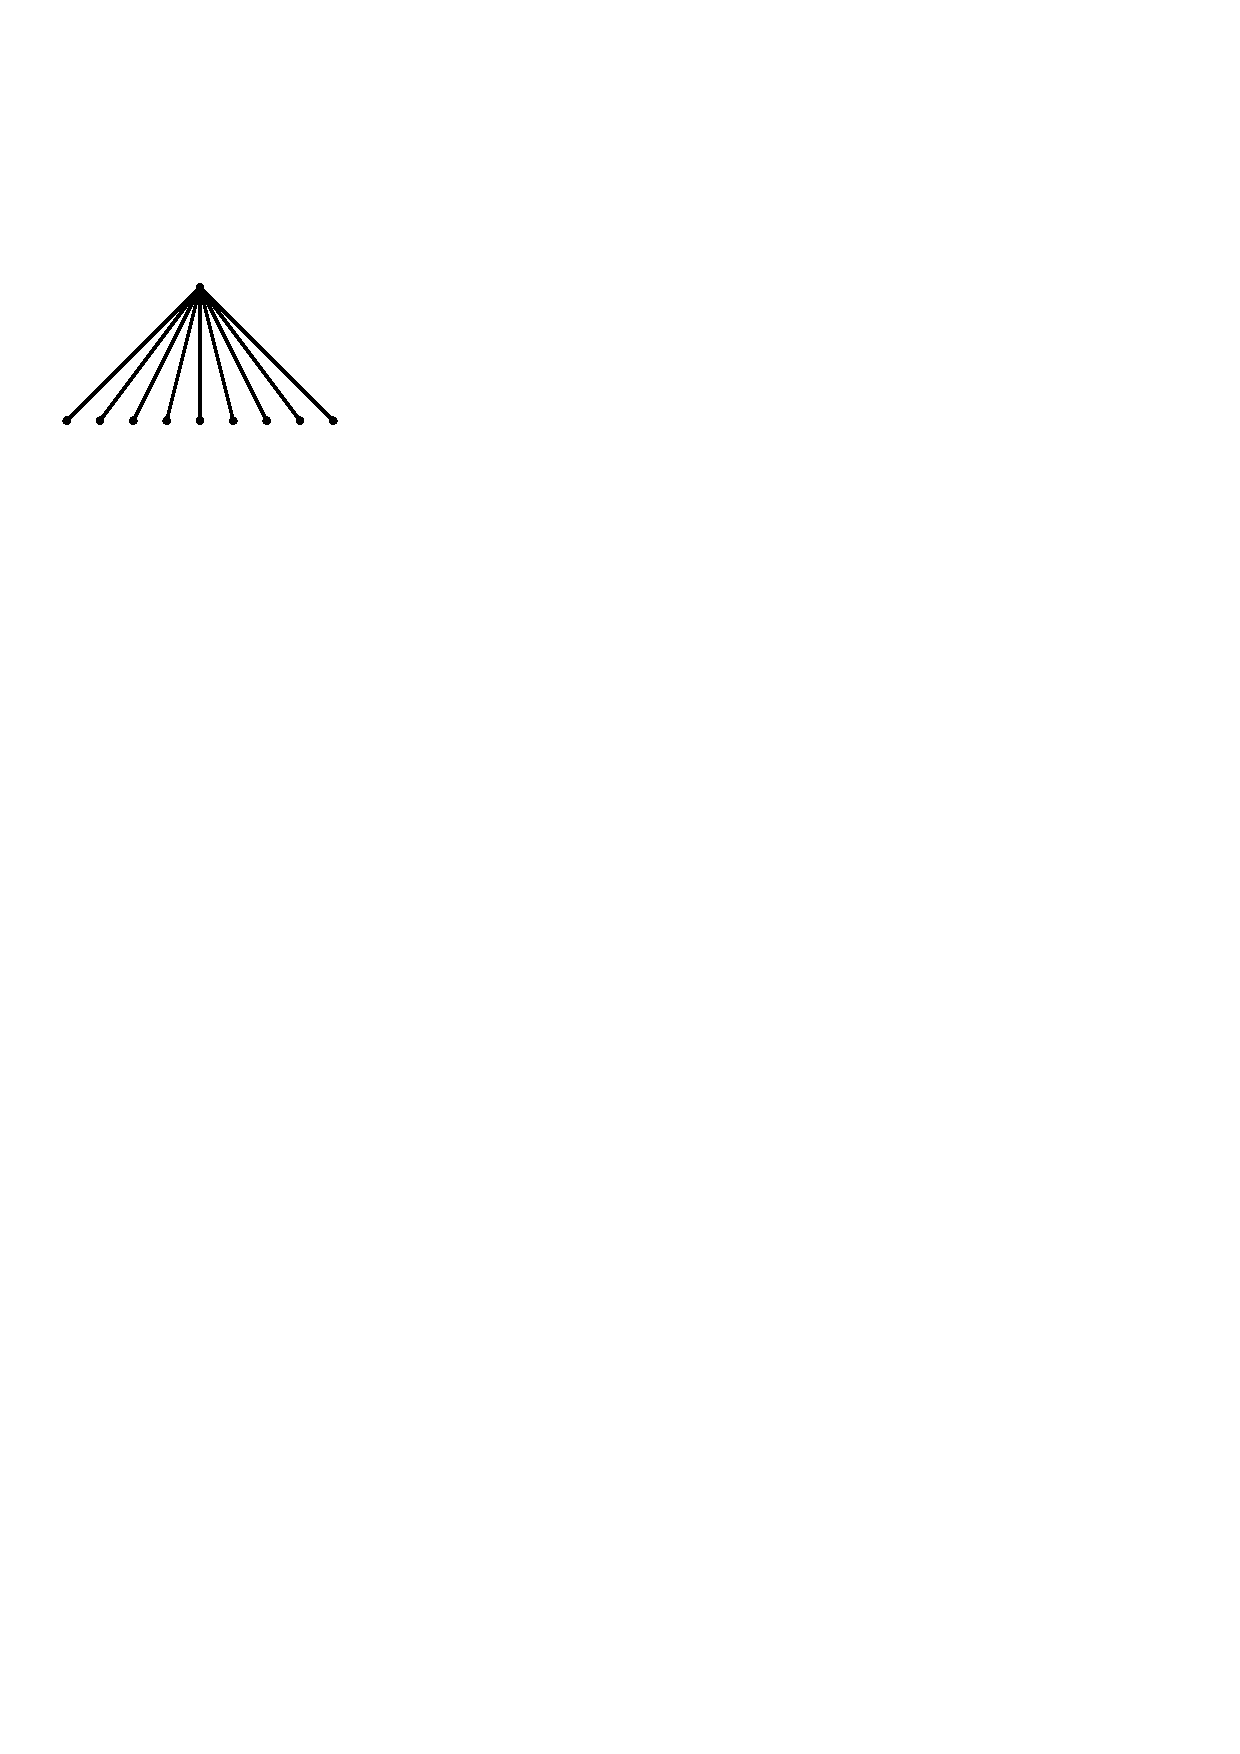
\includegraphics[width=.25\textwidth]{figs/s} & $\CartProd$ & 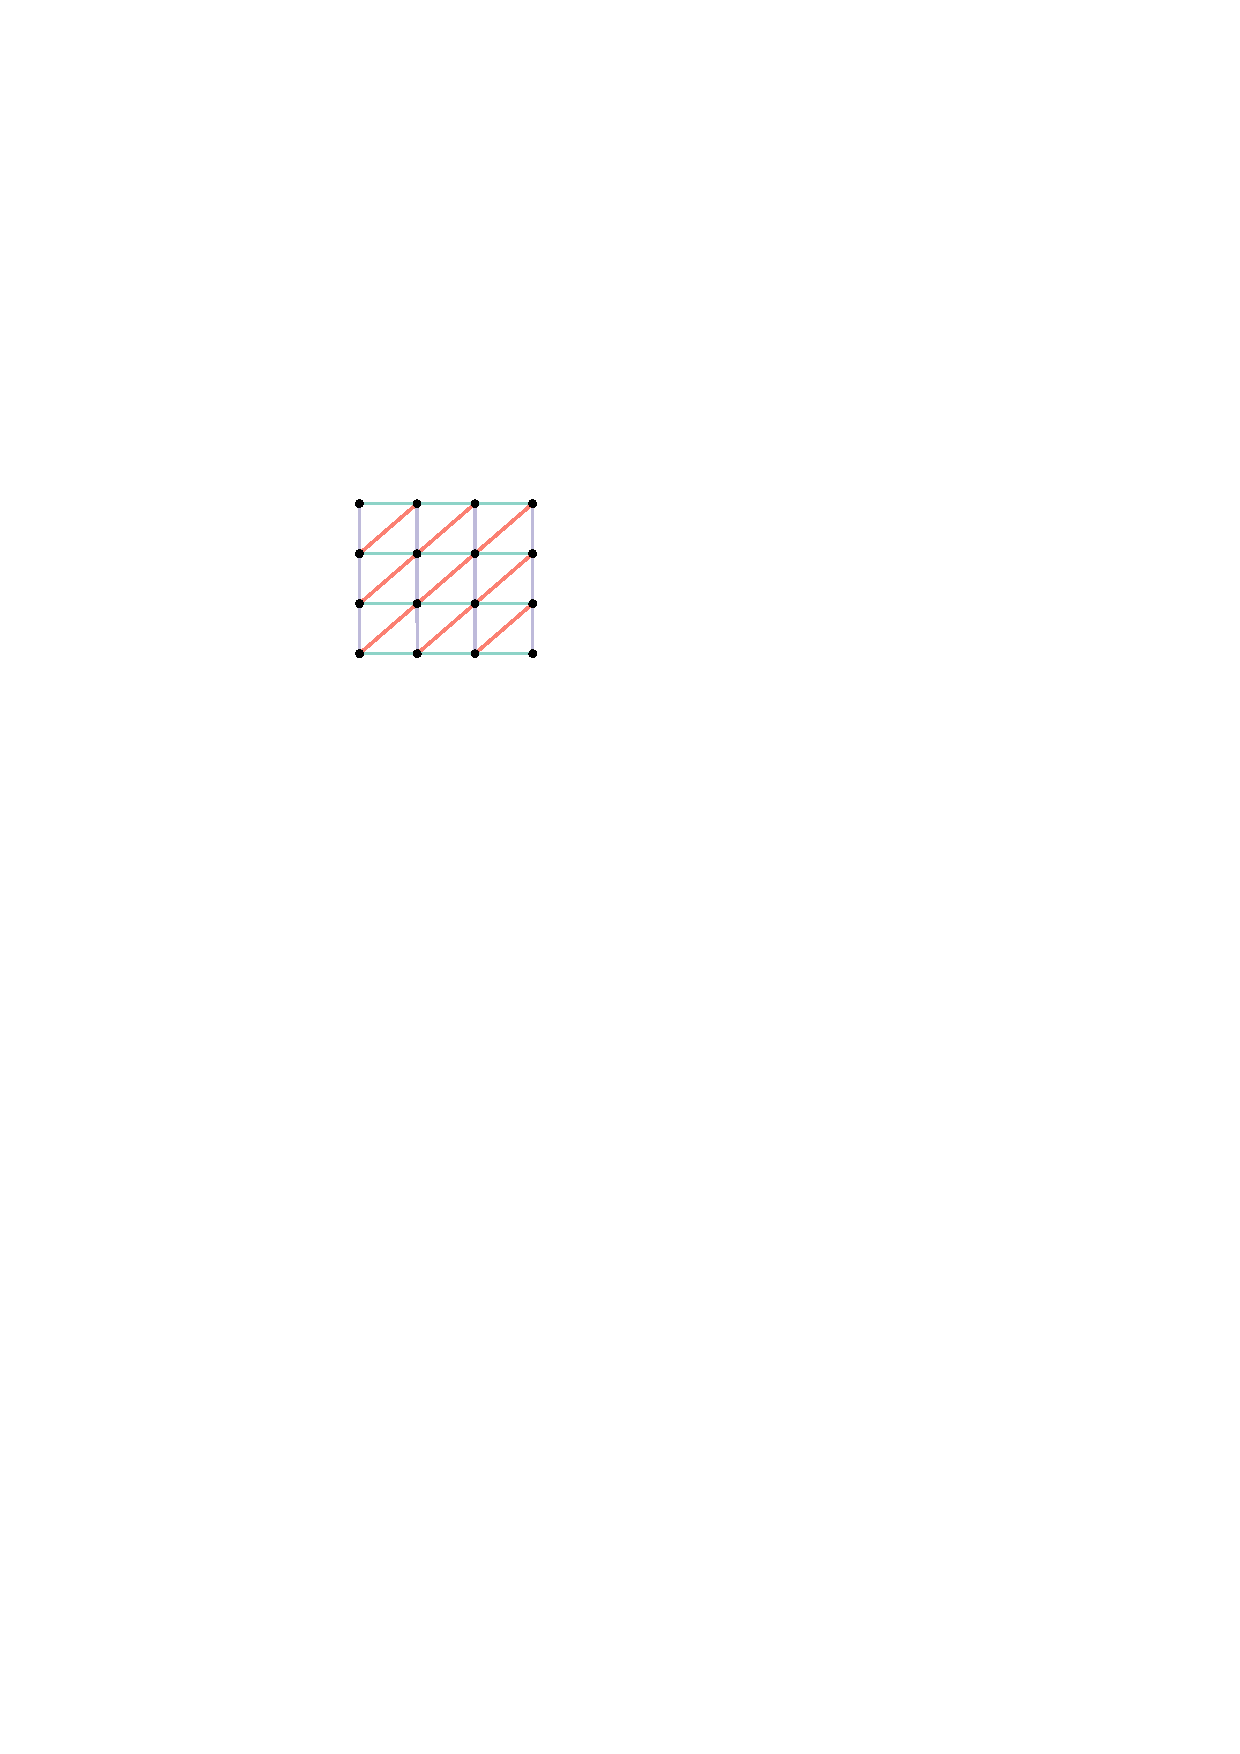
\includegraphics[width=.25\textwidth]{figs/q} & $=$
			& 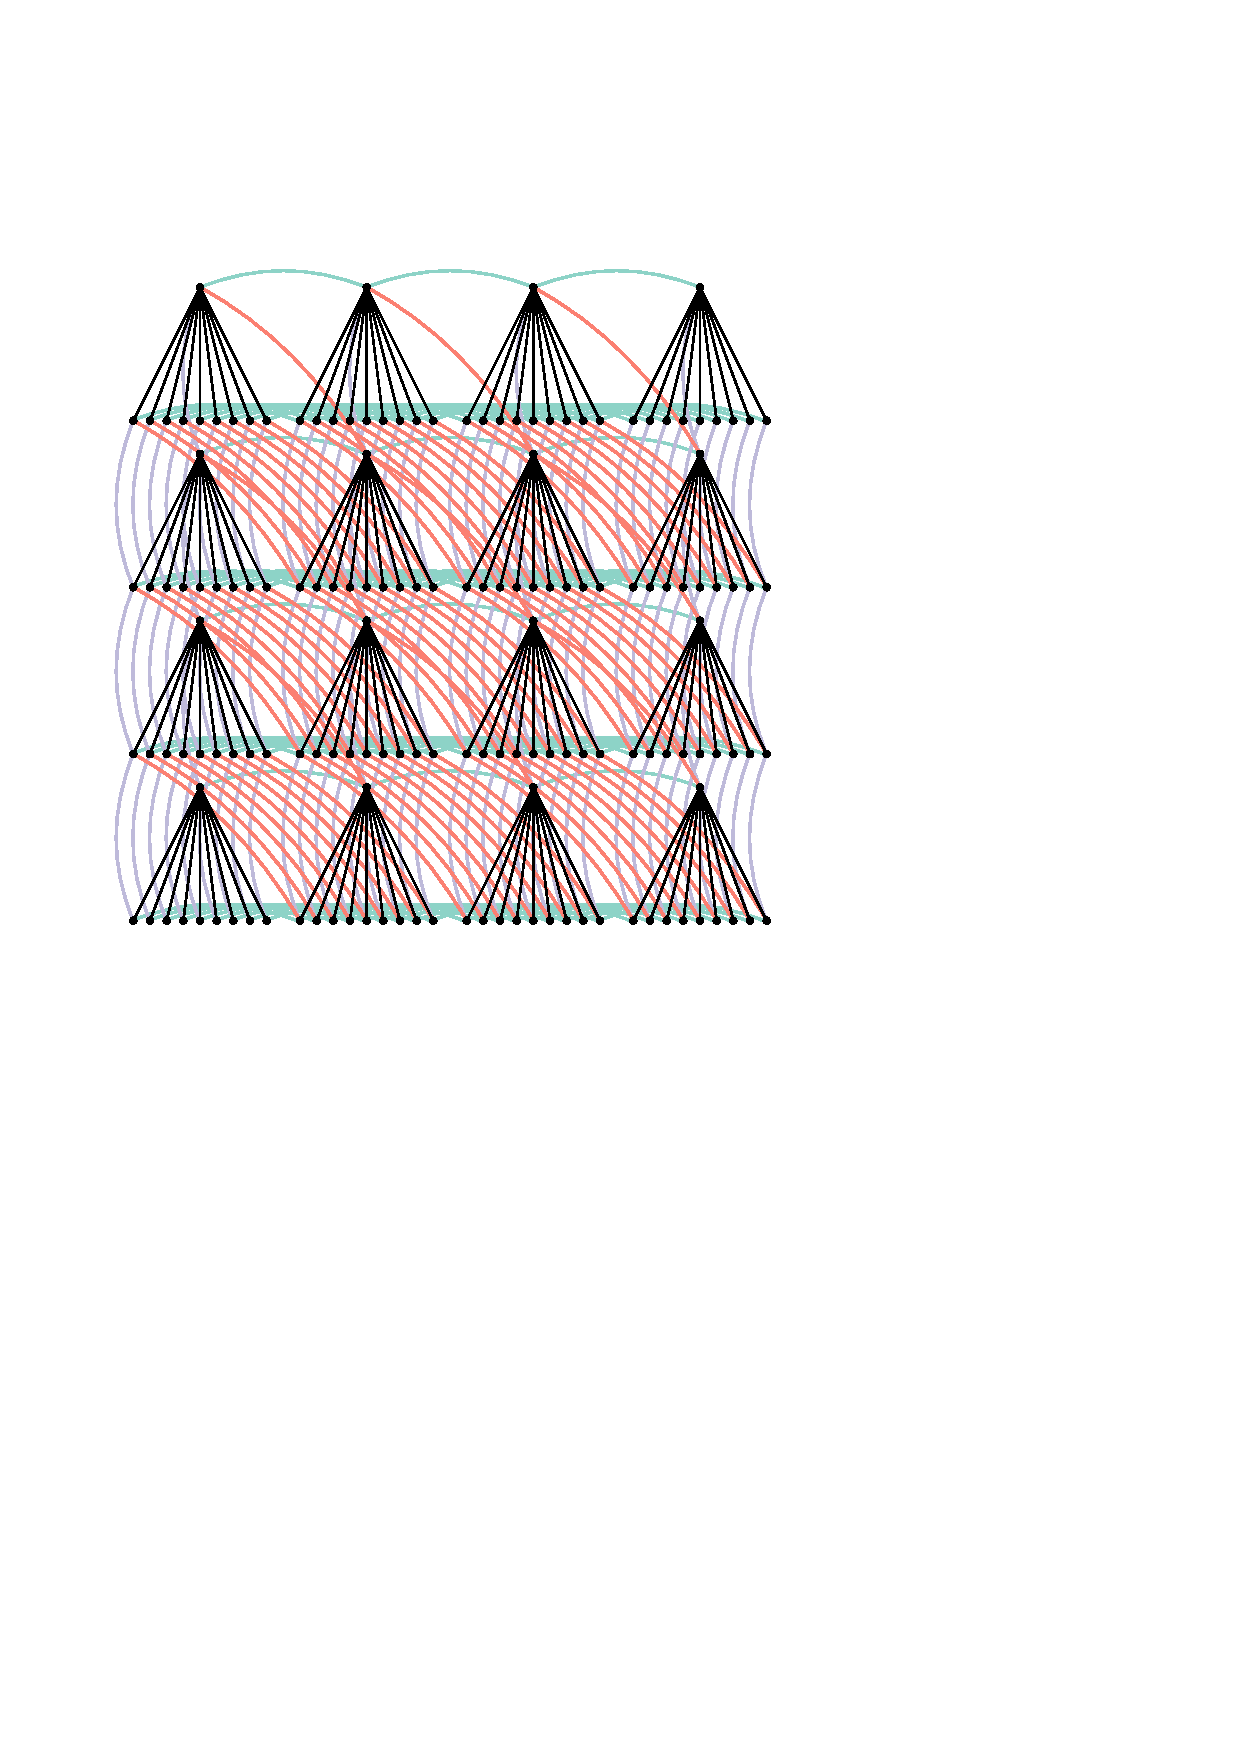
\includegraphics[width=.3\textwidth]{figs/product}
		\end{tabular}
	\end{center}
	% 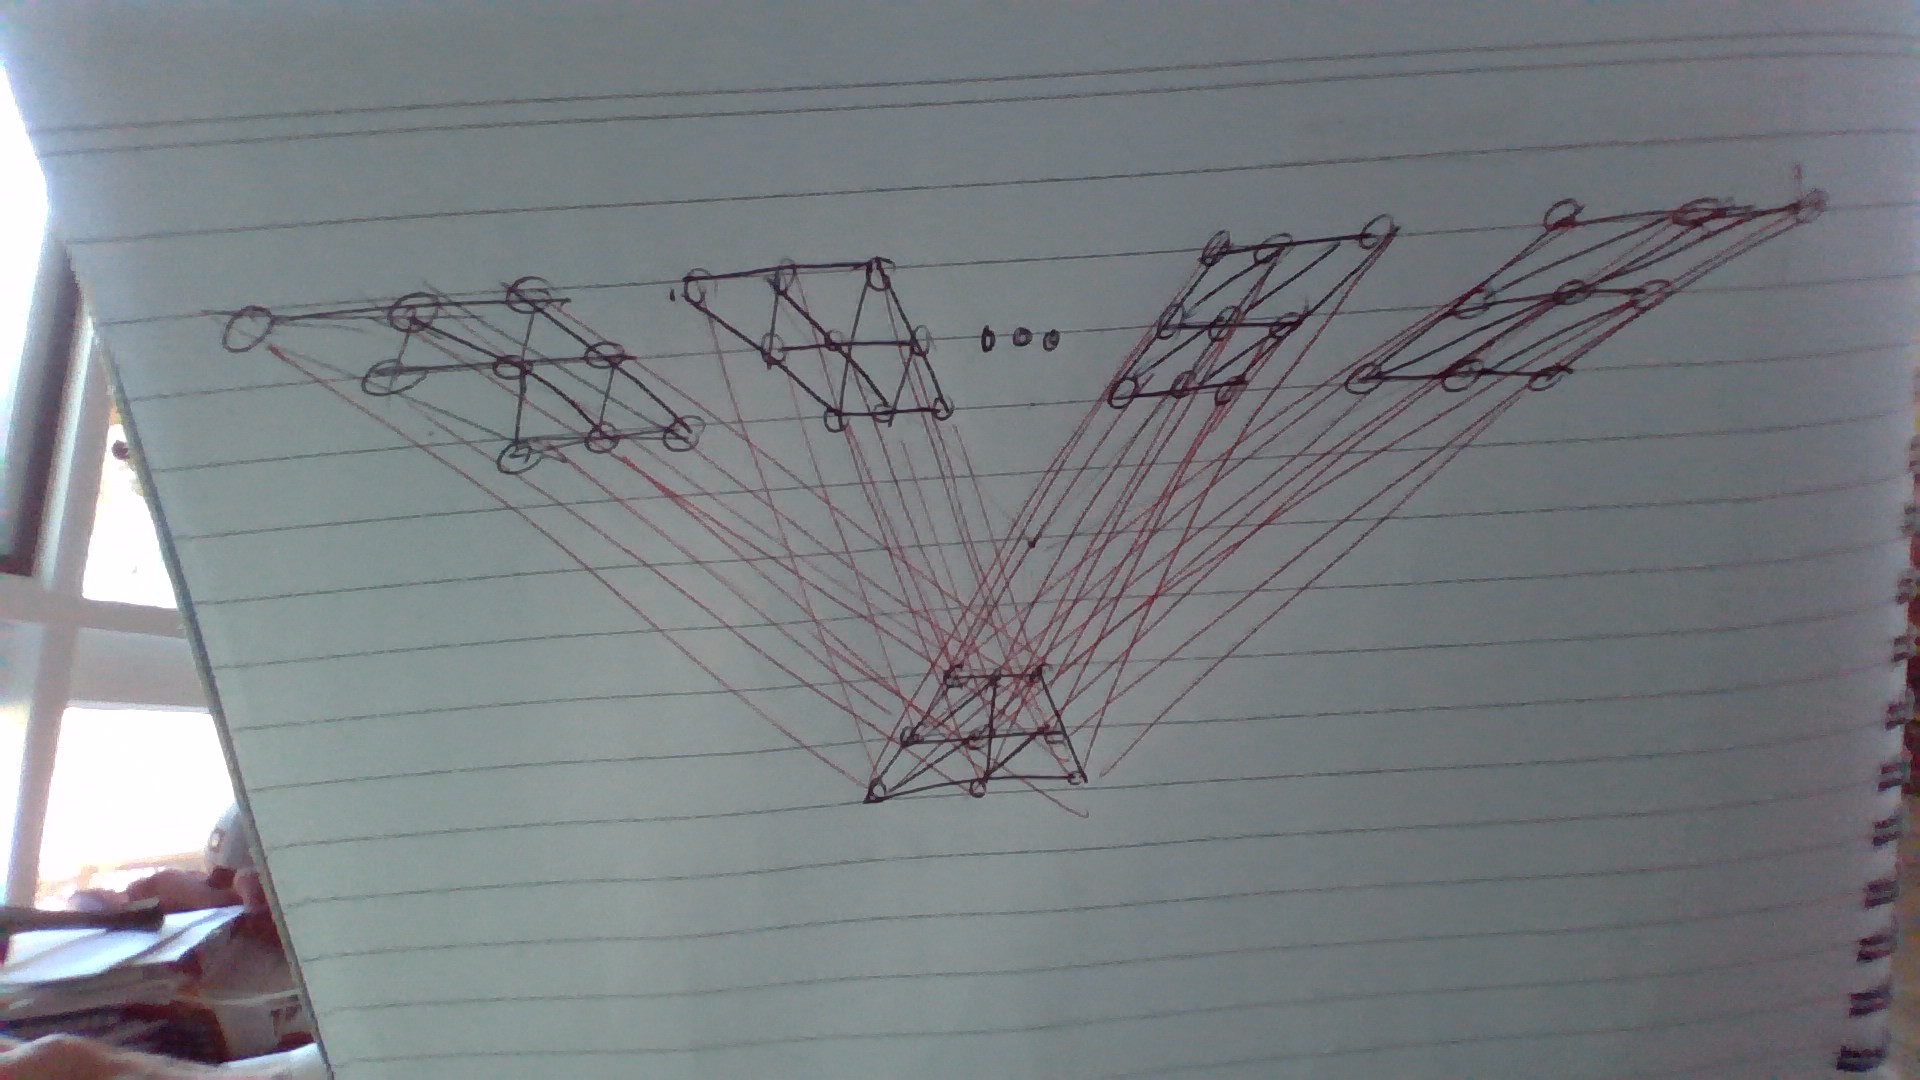
\includegraphics[width=\textwidth]{figs/figure}
	\caption{$S_9 \CartProd H_4$.}
	\label{graph}
\end{figure}


\subsection*{Subdivisions}

A noteworthy consequence of \Cref{family} is that it resolves a conjecture of \citet{BO99}. A graph $G'$ is a \textit{subdivision} of a graph $G$ if $G'$ can be obtained from $G$ by replacing the edges $vw$ of $G$ by internally disjoint paths $P_{vw}$ with endpoints $v$ and $w$. If each $P_{vw}$ has exactly $k$ internal vertices, then $G'$ is the \emph{$k$-subdivision} of $G$. If each $P_{vw}$ has at most $k$ internal vertices, then $G'$ is a \emph{$(\leq k)$-subdivision} of $G$. \citet{BO99} conjectured that the stack-number of $(\leq k)$-subdivisions ($k$ fixed)  is not much less than the stack-number of the original graph. More precisely:

\begin{conj}[\citep{BO99}]
\label{B_conj}
There exists a function $f$ such that for every graph $G$ and integer $k$, if $G'$ is any $(\leq k)$-subdivision of $G$, then $\sn(G) \leq f(\sn(G’),k)$.
\end{conj}

\citet{DujWoo05} established a connection between this conjecture and the question of whether stack-number is bounded by queue-number. In particular, they showed that if
\cref{B_conj} is true, then stack-number is bounded by queue-number. Since \cref{family} shows that stack-number is not bounded by queue-number, \cref{B_conj} is false. The proof of \citet{DujWoo05} is based on the folllowing key lemma: every graph $G$ has a $3$-stack subdivision with $1+2 \ceil{\log_2\qn(G)}$ division vertices per edge. Applying this result to the graph $G=S_b\CartProd H_n$ in \cref{family},
the $5$-subdivision of $S_b\CartProd H_n$ has a $3$-stack layout. If \cref{B_conj} was true, then $\sn(S_b\CartProd H_n) \leq f( 3,5)$, contradicting \cref{family}.

%Specifically,
%\[
%    \mathcal{F} := \{ S_b\square H_n : b,n\in\N\}
%\]
%where $S_b$ denotes the star with $b$ leaves and $H_n$ is the triangulated $n\times n$ grid.

%\todo[inline]{PM: Does anyone know if there is a standard box operator that is typeset like this $S\boxtimes H$ or $S\boxdot H$ instead of like this $S\square H$ or like this $S\Box H$?  I tried square and Box. DW: I defined \texttt{CartProd} which typesets okay $A \CartProd B$	.}


%The graph $G$ in \cref{family} is obtained as follows (See \figref{graph}): Let $S_b$ denote the star graph with root $r$ and $b$ leaves.  For an even positive integer $n$, let $H_n$ be the $n\times n$ triangulated grid, defined by $V(H_n):=\{1,\ldots,n\}^2$ and
%\begin{align*}
%E(H_n) & :=\{(x,y)(x+1,y):x\in\{1,\ldots,n-1\},\,y\in\{1,\ldots,n\}\} \\
%& \qquad \cup \{(x,y)(x,y+1):x\in\{1,\ldots,n\},\,y\in\{1,\ldots,n-1\}\} \\
%& \qquad \cup \{(x,y+1)(x+1,y):x,y\in\{1,\ldots,n-1\}\} \enspace .
%\end{align*}
%We consider the graph $G:=S_b\CartProd H_n$. That is, $V(G)=V(S_b)\times V(H_n)$ where vertices $(v_1,w_1),(v_2,w_2)\in V(G)$ are adjacent whenever $v_1=w_1$ and $v_2w_2\in E(H_n)$, or $v_1w_1\in E(S_b)$ and $v_2=w_2$.


%SAY SOMETHING ABOUT THE RESULTS OF \citet{Pupyrev20}. I EXPECT WE SOLVE SOME OPEN PROBLEM HERE.\todo{PM:Not really, his open problem is about $H\boxtimes P$ where $H$ has bounded treewidth.}

\subsection*{Is Queue-number Bounded by Stack-Number? }

It remains open whether queues are more powerful than stacks; that is, whether queue-number is bounded by stack-number. Several reults are known about this problem. \citet{HLR92} showed that every 1-stack graph has a 2-queue layout. \citet{DJMMUW20} showed that planar graphs have bounded queue-number. (Note that graph products also feature heavily in this proof.)\ Since 2-stack graphs are planar, this implies that 2-stack graphs have bounded queue-number. It is open whether 3-stack graphs have bounded queue-number. In fact, the case of three stacks is as hard as the general question. \citet{DujWoo05} proved that queue-number is bounded by stack-number if and only if 3-stack graphs have bounded queue-number. Moreover, if this is true then stack-number is bounded by a polynomial function of queue-number.


\section{Stack and Queue Layouts of Cartesian Products}

\todo[inline]{Add discussion of result of \citet{BK79}: $\sn(G\CartProd H) \leq \sn(G) + \dsn(H)$ for bipartite $H$. Highlight the key difference between stack and queue layouts is that we need $H$ to be bipartite here.}

\todo{mention results of \citet{Pupyrev20} about bipartite graphs?}

First we prove that $\qn(S_b\CartProd H_n)\leq 4$, as claimed in \cref{family}. We need the following definition due to \citet{Wood-Queue-DMTCS05}. A queue layout $(\varphi,\prec)$ is \emph{strict} if for every vertex $u\in V(G)$ and for all neighbours $v,w\in N_G(u)$, if $u\prec v,w$ or $v,w \prec u$, then $\varphi(uv)\neq \varphi(uw)$. Let $\sqn(G)$ be the minimum integer $k$ such that $G$ has a strict $k$-queue layout. To see that $\sqn(H_n) \leq 3$, order the vertices row-by-row and then left-to-right within a row, with vertical edges in one queue, horizontal edges in one queue, and diagonal edges in another queue.
\citet{Wood-Queue-DMTCS05} proved that $\qn(G\CartProd H) \leq \qn(G) + \sqn(H)$ for all graphs $G$ and $H$. Of course, $S_b$ has a 1-queue layout (since no two edges are nested for any vertex-ordering). Thus $\qn(S_b \CartProd H_n)\leq 4$.

\section{The Main Proof}

We now turn to the proof of our main result, the lower bound on $\sn(G)$, where $G:= S_b\CartProd H_n$. Consider a hypothetical $s$-stack layout $(\varphi,\prec)$ of $G$ where $n$ and $b$ are chosen sufficiently large compared to $s$ as detailed below. We begin with three lemmata that, for sufficiently large $b$, provide a large subgraph $S_d$ of $S_b$ for which the induced stack layout of $S_d\CartProd H_n$ is highly structured.

For each node $v$ of $S_b$, define $\pi_v$ as the permutation of $\{1,\ldots,n\}^2$ in which $(x_1,y_1)$ appears before $(x_2,y_2)$ if and only if $(v,(x_1,y_1))\prec (v,(x_2,y_2))$. The following lemma is an immediate consequence of the Pigeonhole Principle:

\begin{lem}\lemlabel{uniform_order}
    There exists a permutation $\pi$ of $\{1,\ldots,n\}^2$ and a set $L_1$ of leaves of $S_b$ of size $a\ge b/(n^2)!$ such that $\pi_{v}=\pi$ for each $v\in L_1$.
\end{lem}

% \todo[inline]{If we cared, we could improve this to $b/2^{cn^2}$ since we only use the weaker property (P3) in the final proof. DW: I don't care. }

For each leaf $v$ in $L_1$, let $\varphi_v$ be the edge colouring of $H_n$ defined by $\varphi_v(xy):=\varphi((v,x)(v,y))$ for each $xy\in E(H_n)$. Since $H_n$ has maximum degree $6$ and is not 6-regular, it has fewer than $3n^2$ edges.  Therefore there are fewer than $s^{3n^2}$ edge colourings of $H_n$ using $s$ colours.  Another application of the Pigeonhole Principle proves the following:

\begin{lem}\lemlabel{uniform_colour}
    There exists a subset $L_2\subseteq L_1$ of size $c\ge a/s^{3n^2}$
    and an edge colouring $\phi:E(H_n)\to\{1,\ldots,s\}$ such that $\varphi_v=\phi$ for each $v\in L_2$.
\end{lem}


Let $S_{c}$ be the subgraph of $S_b$ induced by $L_2\cup\{r\}$. The preceding two lemmata ensure that, for distinct leaves $v$ and $w$ of $S_{c}$, the stack layouts of the isomorphic graphs $G[\{(v,p):p\in V(H_n)\}]$ and $G[\{(w,p):p\in V(H_n)\}]$ are identical. The next lemma is a statement about the relationships between the stack layouts of $G[\{(v,p):v\in V(S_{c})\}]$ and $G[\{(v,q):v\in V(S_{c})\}]$ for  distinct $p,q\in V(H_n)$.  It does not assert that these two layouts are identical but it does state that they fall into one of two categories.

\begin{lem}\lemlabel{forward_or_backward}
    There exists a sequence $L_3:=u_1,\ldots,u_{d}$ with $\{u_1,\ldots,u_{d}\}\subseteq L_2$ of length $d\ge c^{1/2^{n^2-1}}$ such that, for each $p\in V(H_n)$, either  $(u_1,p)\prec (u_2,p)\prec\cdots\prec (u_{d},p)$ or $(u_1,p)\succ (u_2,p)\succ\cdots\succ (u_{d},p)$.
\end{lem}

\begin{proof}
    Let $p_1,\ldots,p_{n^2}$ denote the vertices of $H_n$ in any order.
    Begin with the sequence $S_1:=v_{1,1},\ldots,v_{1,c}$ that contains all $c$ elements of $L_2$ ordered so that $(v_{1,1},p_1)\prec\cdots\prec(v_{1,c},p_1)$.  For each $i\in\{2,\ldots,n^2\}$, the Erd\H{o}s-Szekeres Theorem~\citep{ES35} implies that $S_{i-1}$ contains a subsequence $S_i:=v_{i,1},\ldots,v_{i,|S_i|}$ of length $|S_i|\ge \sqrt{|S_{i-1}|}$ such that $(v_{i,1},p_i)\prec\cdots\prec(v_{i,|S_i|},p_i)$ or $(v_{i,1},p_i)\succ\cdots\succ(v_{i,|S_i|},p_i)$.  It is straightforward to verify by induction on $i$ that $|S_i| \ge c^{1/2^{i-1}}$ resulting in a final sequence $S_{n^2}=:L_3$ of length at least $c^{1/2^{n^2-1}}$.
\end{proof}

For the rest of the proof we will work with the star $S_d$ whose leaves are $u_1,\ldots,u_d$ described in \lemref{forward_or_backward}.  Consider the (improper) vertex colouring of $H_n$ obtained by colouring each vertex $p\in V(H_n)$ \emph{red} if $(u_1,p)\prec\cdots\prec (u_d,p)$ and colouring $p$ \emph{blue} if $(u_1,p)\succ\cdots\succ(u_d,p)$. We need the following famous Hex Lemma~\citep{Gale79}.

\begin{lem}[\citep{Gale79}] \label{hex_lemma}
Every red--blue vertex colouring of the graph $H_n$	contains an $n$-vertex path $R$ consisting entirely of red vertices or entirely of blue vertices.
\end{lem}

%\begin{proof}
%    The dual of $H_n$ is the board on which the game Hex is played.  The well-known \emph{Hex Lemma} states that any colouring of the vertices of $H_n$ with colours red and blue contains exactly one of the following \cite{Gale79}:
%    \begin{compactenum}
%        \item a path with endpoints $(x,1)$ and $(x',n)$ consisting entirely of red vertices, for some $x,x'\in\{1,\ldots,n\}$; or
%        \item a path with endpoints $(1,y)$ and $(n,y')$ consisting entirely of blue vertices, for some $y,y'\in\{1,\ldots,n\}$.
%    \end{compactenum}
%    In either case, the path contains at least $n$ vertices and therefore has a $n$-vertex subpath consisting entirely of red vertices or entirely of blue vertices.
%\end{proof}

Without loss of generality, assume that the path $R:=p_1,\ldots,p_n$ defined by \cref{hex_lemma} (with the above-defined colouring) consists entirely of red vertices, so that $(u_1,p_j)\prec\cdots\prec (u_d,p_j)$ for each $j\in\{1,\ldots,n\}$.  Recall that $(\varphi,\prec)$ is a hypothetical $s$-stack layout of $G$ and therefore it is also an $s$-stack layout of the subgraph $X:=S_d\CartProd R$. In particular, there is no set of greater than $s$ pairwise crossing edges in $X$. The following result finishes the proof by showing that such a set exists when $n> 2s$ and $d\ge (s+1)2^{n}$ (which is implied if $n=2s+1$ and $b \ge (n^2)!\, s^{3n^2}\, ((s+1)2^n)^{2^{n^2-1}} $).


\begin{lem}\lemlabel{twister}
    The graph $X$ contains a set of edges of size at least $\min\{\lfloor d/2^{n}\rfloor,\lceil n/2\rceil\}$ that are pairwise crossing with respect to $\prec$.
\end{lem}

\begin{proof}
	Extend the total order $\prec$ onto a partial order over subsets of $V(G)$ so that, for $V,W\subseteq V(G)$,  $V\prec W$ if and only if $v\prec w$ for each $v\in V$ and each $w\in W$.  We abuse notation slightly by using $\prec$ to compare elements of $V(G)$ and subsets of $V(G)$ so that, for $v\in V(G)$ and $V\subseteq V(G)$, $v\prec V$ denotes $\{v\}\prec V$.
    We will define sets $A_1\supseteq \cdots\supseteq A_{n}$ of leaves of $S_d$ so that each $A_i$ satisifies the following conditions:
    \begin{compactenum}[(C1)]
        \item $A_i$ contains $d_i\ge d/2^{i-1}$ leaves of $S_d$.
        \item Each leaf $v\in A_i$ defines an $i$-element vertex set $Z_{i,v}:=\{(v,p_j):j\in\{1,\ldots,i\}\}$.  For any distinct $v,w\in A_i$, the sets $Z_{i,v}$ and $Z_{i,w}$ are \emph{separated} with respect to $\prec$; that is, $Z_{i,v}\prec Z_{i,w}$ or $Z_{i,v}\succ Z_{i,w}$.
    \end{compactenum}

    Before defining $A_1,\ldots,A_n$ we first show how the existence of the set $A_n$ implies the lemma.  To avoid triple-subscripts, let $d':=d_n\ge d/2^{n-1}$.   The set $A_n$ defines vertex sets $Z_{n,v_1}\prec\cdots\prec Z_{n,v_{d'}}$.  Refer to \figref{twister}. Recall that $r$ is the root of $S_b$ so it is adjacent to each of $v_{1},\ldots,v_{d'}$ in $S_d$.  Therefore, for each $j\in\{1,\ldots,n\}$ and each $i\in\{1,\ldots,d'\}$, the edge $(r,p_j)(v_i,p_j)$ is in $X$. Therefore, $(r,p_j)$ is adjacent to an element of each of $Z_{n,v_1},\ldots,Z_{n,v_{d'}}$.
	\begin{figure}
		\begin{center}
			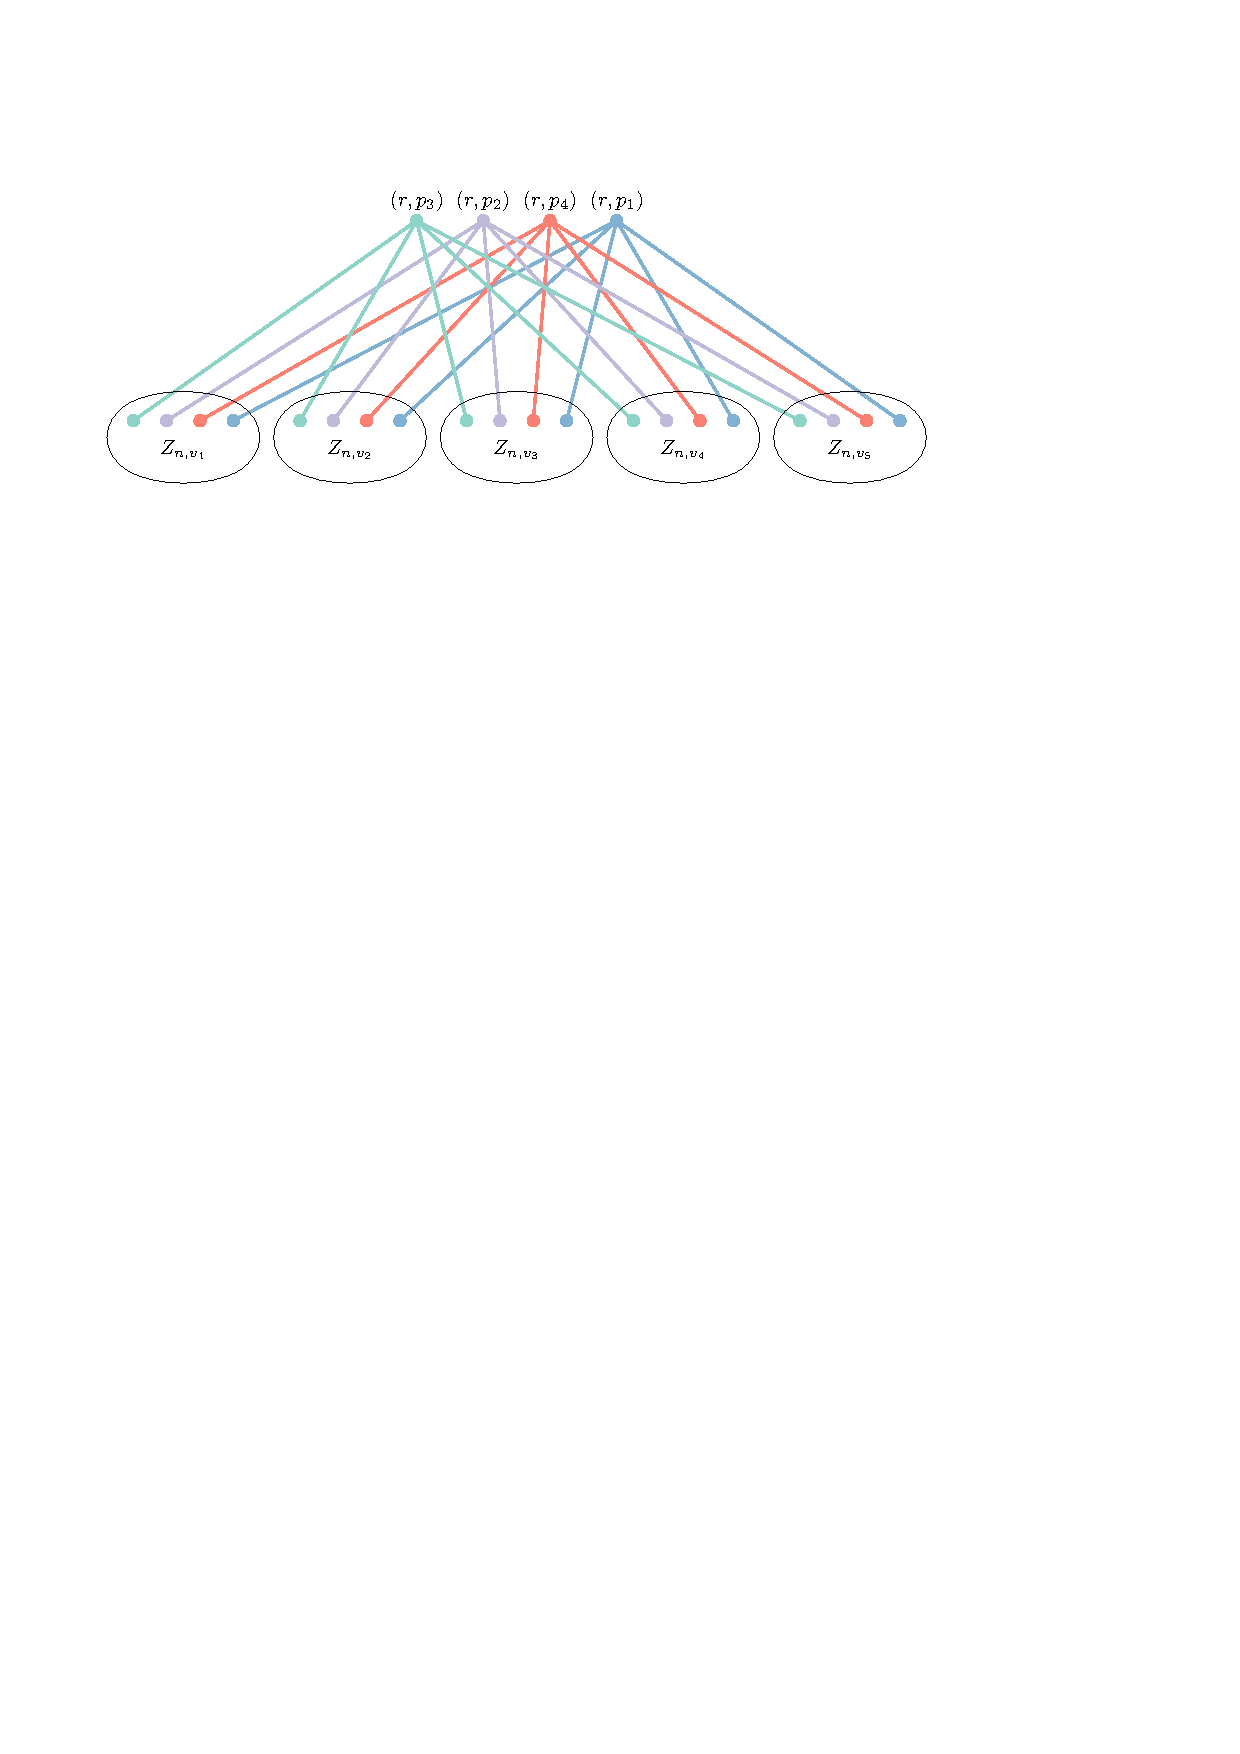
\includegraphics{figs/twister}
		\end{center}
		\caption{The sets $Z_{n,v_1},\ldots,Z_{n,v_{d'}}$ ($n=4$, $d'=5$).}
		\figlabel{twister}
	\end{figure}

    Since $Z_{n,v_1},\ldots,Z_{n,v_{d'}}$ are separated with respect to $\prec$, when viewed from afar, this situation looks like a complete bipartite graph $K_{n,d'}$ with the root vertices $L:=\{(r,p_j):j\in\{1,\ldots,n\}\}$ in one part and the groups $R:=Z_{n,v_1}\cup\cdots\cup Z_{n,v_{d'}}$ in the other part.  Any linear ordering of $K_{n,d'}$ has a large set of pairwise crossing edges so, intuitively, the induced subgraph $X[L\cup R]$ should also have a large set of pairwise crossing edges. We can formalize this as follows: Label the vertices in $L$ as $r_1,\ldots,r_n$ so that $r_1\prec \cdots\prec r_{n}$.  Then at least one of the following two cases applies (see \figref{median}):
    \begin{enumerate}
        \item $Z_{n,\lfloor d'/2\rfloor}\prec r_{\lceil n/2\rceil}$ in which case the graph between $r_{\lceil n/2\rceil},\ldots,r_{n}$ and $Z_{n,1},\ldots,Z_{n,\lfloor d'/2\rfloor}$ has a set of at least $\min\{\lfloor d'/2\rfloor,\lceil n/2\rceil\}$ pairwise-crossing edges.
        \item $r_{\lceil n/2\rceil}\prec Z_{\lceil d'/2\rceil+1}$ in which case the graph between $r_1,\ldots,r_{\lceil n/2\rceil}$ and $Z_{\lceil d'/2\rceil+1},\ldots,Z_{d'}$ has a set of $\min\{\lfloor d'/2\rfloor,\lceil n/2\rceil\}$ pairwise-crossing edges.
    \end{enumerate}
	\begin{figure}
		\begin{center}
			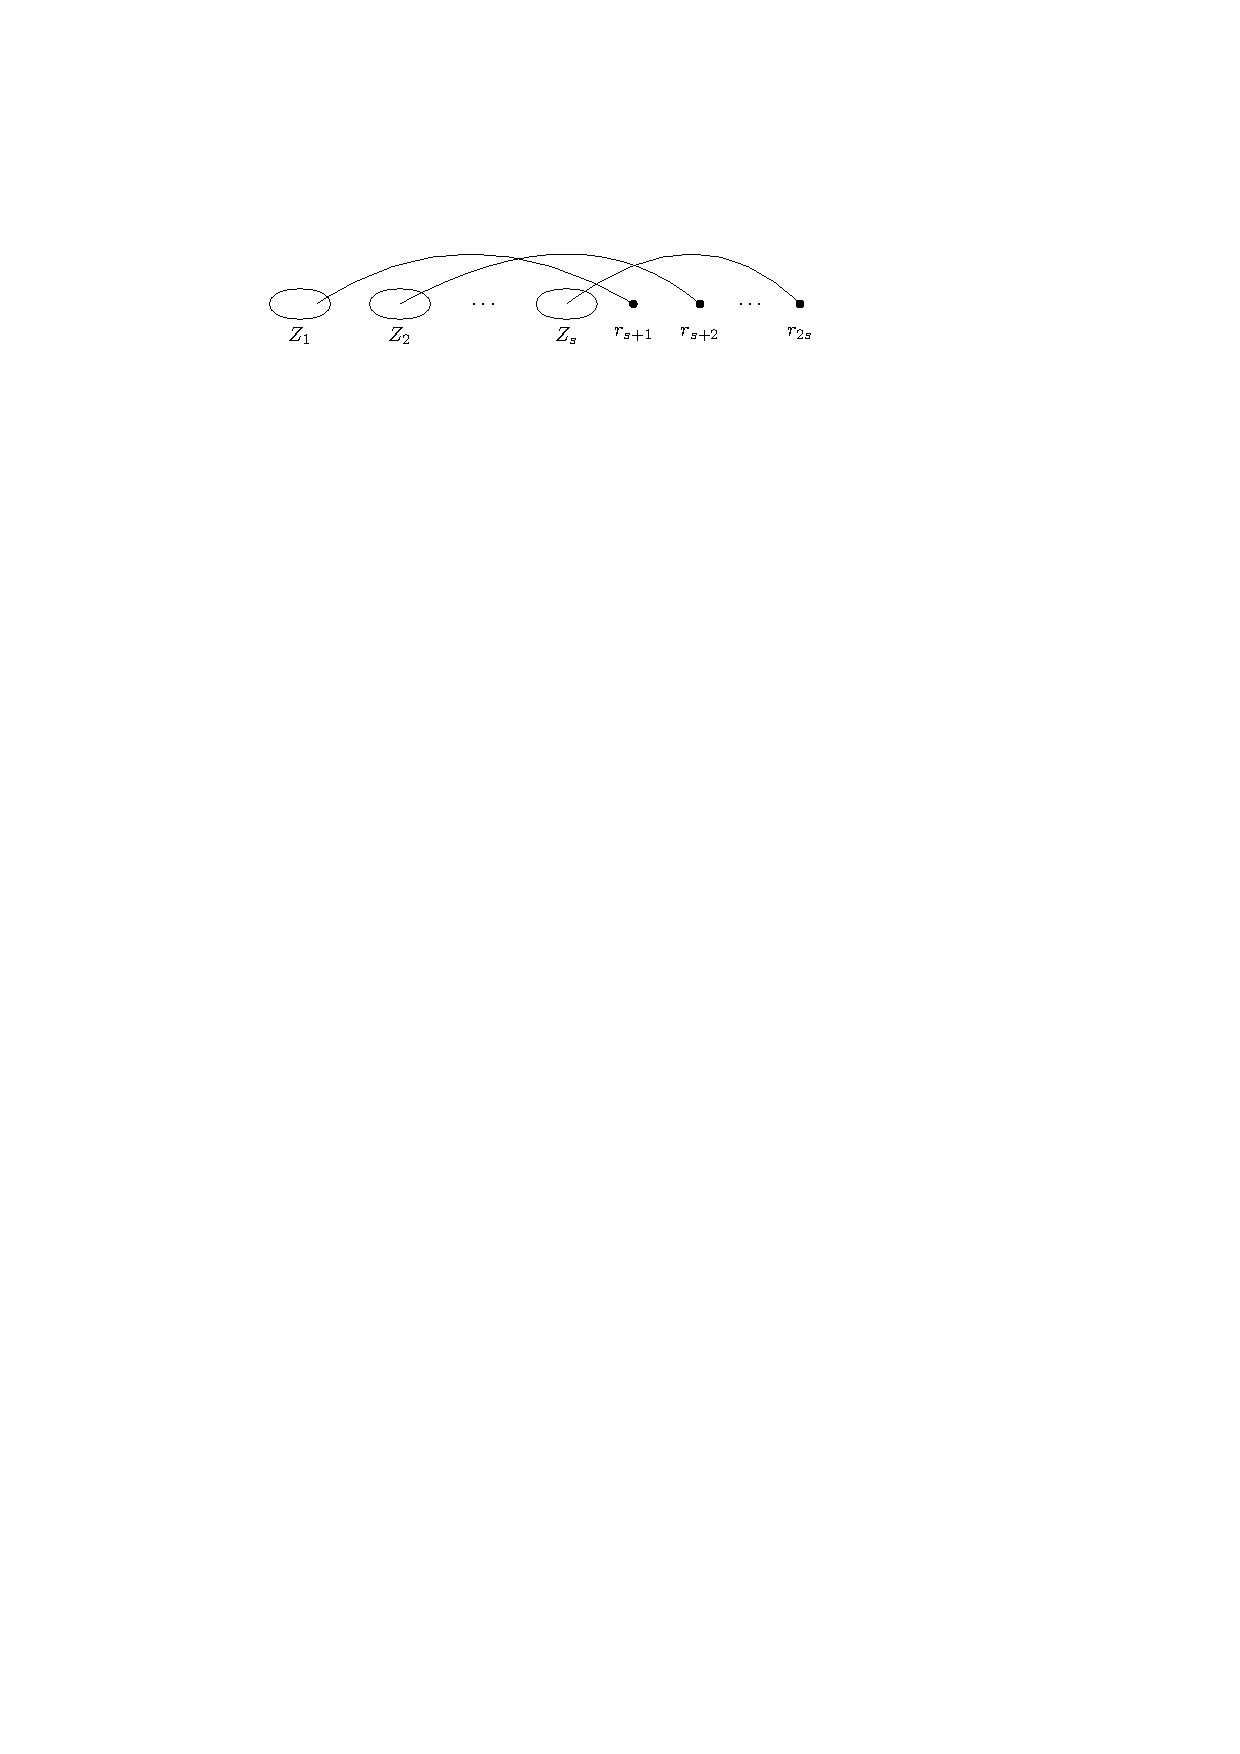
\includegraphics{figs/median-1} \\ 1 \\[2em]
			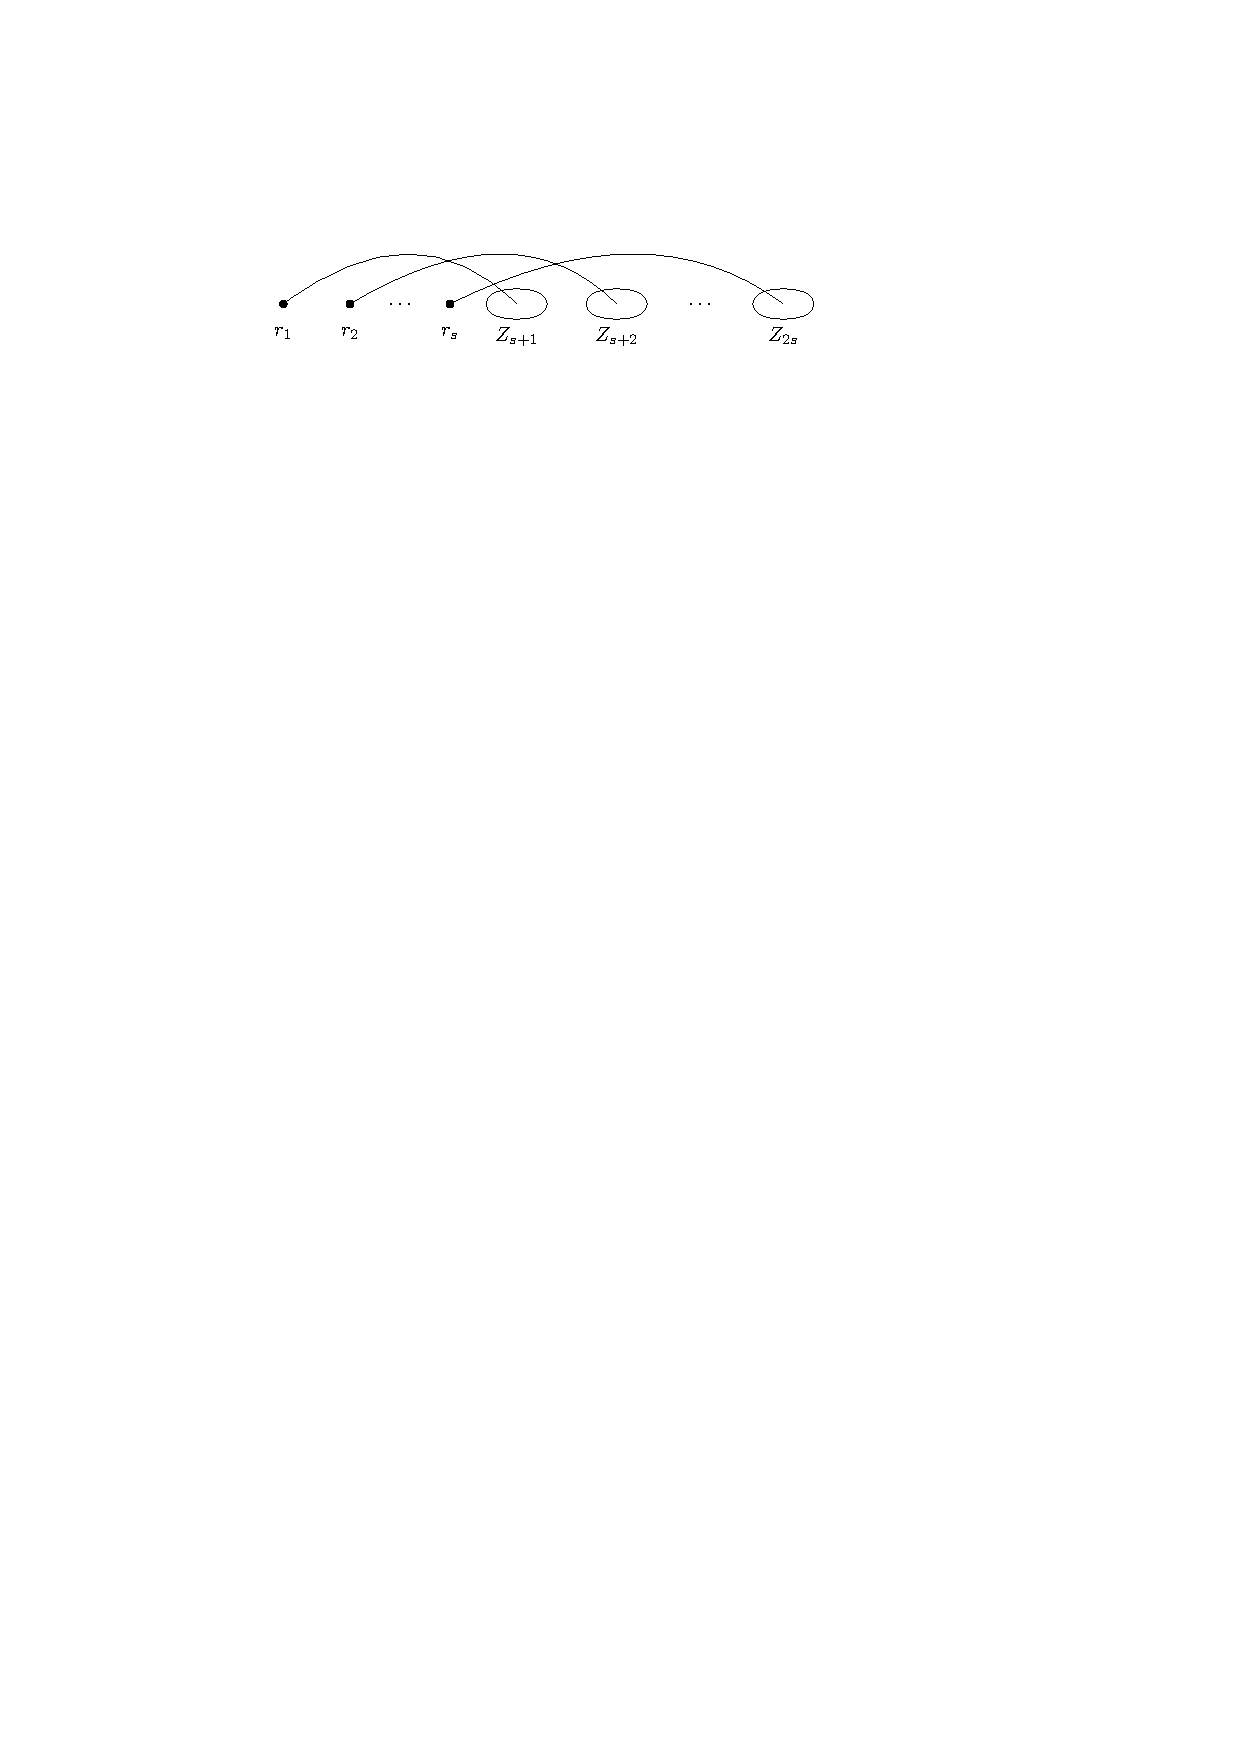
\includegraphics{figs/median-2} \\ 2
		\end{center}
		\caption{The two cases in the proof of \lemref{twister}.}
		\figlabel{median}
	\end{figure}
	Since, by (C1), $d'\ge d/2^{n-1}$, either case results in a set of pairwise-crossing edges of size at least $\min\{\lfloor d/2^n\rfloor,\lceil n/2\rceil\}$, as claimed.

    All that remains is to define the sets $A_1\supseteq\cdots\supseteq A_n$ that satisfy (C1) and (C2).  Let $A_1$ be the set of all the leaves of $S_d$.  For each $i\in\{2,\ldots,n\}$, the set $A_i$ is defined as follows:  Let $Z_1,\ldots,Z_{|A_{i-1}|}$ denote the sets $Z_{i-1, v}$ for each $v\in A_{i-1}$ ordered so that $Z_1\prec\cdots\prec Z_{|A_{i-1}|}$. By Property (C2), this is always possible.	Label the vertices of $A_{i-1}$ as $v_1,\ldots,v_{|A_{i-1}|}$ so that $(v_1,p_{i-1})\prec\cdots\prec (v_r,p_{i-1})$.   (This is equivalent to naming them so that $(v_j,p_{i-1})\in Z_j$ for each $j\in\{1,\ldots,|A_{i-1}|\}$.)  Define the set $A_i:=\{v_{2k+1}:k\in\{0,\ldots,\lfloor(|A_{i-1}|-1)/2\rfloor\}\}=\{v_{j}\in A_{i-1}:\text{$j$ is odd}\}$.  This completes the definition of $A_1,\ldots,A_n$.

	All that remains is to verify that $A_i$ satisfies (C1) and (C2) for each $i\in\{1,\ldots,n\}$.  We do this by induction on $i$. The base case $i=1$ is trivial so we assume from this point on that $i\in\{2,\ldots,n\}$.   To see that $A_i$ satisfies (C1) just observe that $|A_i|=\lceil |A_{i-1}|/2\rceil \ge |A_{i-1}|/2\ge d/2^{i-1}$, where the final inequality follows by applying the inductive hypothesis $|A_{i-1}|\ge d/2^{i-2}$.  Now all that remains is to show that $A_i$ satisfies (C2).

    Recall that, for each $v\in A_{i-1}$, the edge $e_v:=(v,p_{i-1})(v,p_i)$ is in $X$.  We have the following properties:
    \begin{compactenum}[(P1)]
        \item By \lemref{uniform_colour}, $\varphi(e_v)=\phi(p_{i-1}p_i)$ for each $v\in A_{i-1}$.
        \item Since $p_{i-1}$ and $p_i$ are both red, $(v,p_{i-1})\prec (w,p_{i-1})$ if and only if $(v,p_{i})\prec (w,p_{i})$ for each $v,w\in A_{i-1}$.
        \item By \lemref{uniform_order}, $(v,p_{i-1})\prec (v,p_i)$ for every $v\in A_{i-1}$ or $(v,p_{i-1})\succ (v,p_i)$ for every $v\in A_{i-1}$.
    \end{compactenum}
    We claim that these three conditions imply that the vertex sets $\{(v,p_{i-1}):v\in A_{i-1}\}$ and $\{(v,p_i):v\in A_{i-1}\}$ interleave perfectly with respect to $\prec$. More precisely:
	\begin{clm}\clmlabel{interleave} $(v_1,p_{i-1+t})\prec (v_1,p_{i-t}) \prec (v_2,p_{i-1+t}) \prec (v_2,p_{i-t}) \cdots \prec (v_r,p_{i-1+t}) \prec (v_r,p_{i-t})$ for some $t\in\{0,1\}$.
	\end{clm}
	\begin{proof}[Proof of \clmref{interleave}]
		By (P3) we may assume, without loss of generality, that $(v,p_{i-1})\prec (v,p_i)$ for each $v\in A_{i-1}$, in which case we are trying to prove the claim for $t=0$.  Therefore, it is sufficient to show that $(v_j,p_i)\prec (v_{j+1},p_{i-1})$ for each $j\in\{1,\ldots,r-1\}$.  For the sake of contradiction, suppose $(v_j,p_{i})\succ (v_{j+1},p_{i-1})$ for some $j\in\{1,\ldots,r-1\}$. By the labelling of $A_{i-1}$,  $(v_j,p_{i-1})\prec (v_{j+1},p_{i-1})$ so, by (P2),  $(v_{j},p_i) \prec (v_{j+1},p_i)$.  Therefore
		\[
			(v_j,p_{i-1})\prec (v_{j+1},p_{i-1})\prec(v_{j},p_i) \prec
		   (v_{j+1}, p_i) \enspace .
	   	\]
		Therefore the edges $e_{v_j}=(v_j,p_{i-1})(v_j,p_{i})$ and $e_{v_{j+1}}=(v_{j+1},p_{i-1})(v_{j+1},p_i)$ cross with respect to $\prec$.  But this is a contradiction since, by (P1),  $\varphi(e_{v_j}) =\varphi(e_{v_{j+1}})=\phi(p_{i-1}p_i)$.
		This contradiction completes the proof of \clmref{interleave}.
	\end{proof}

% \todo{DW: Why are these $\prec$'s red?  PM: Just me keeping track of which one was the assumption, they don't need to be red.}

We now complete the proof that $A_i$ satisfies (C2). Apply \clmref{interleave} and assume without loss of generality that $t=0$, so that
	\[
		(v_1,p_{i-1})\prec (v_1,p_{i}) \prec (v_2,p_{i-1}) \prec (v_2,p_{i}) \cdots \prec (v_r,p_{i-1}) \prec (v_r,p_{i}) \enspace .
	\]

    For each $j\in\{1,\ldots,r-2\}$, we have $(v_{j+1},p_{i-1})\in Z_{j+1}\prec Z_{j+2}$, so  $(v_j,p_i)\prec (v_{j+1},p_{i-1}) \prec Z_{j+2}$.  Therefore $Z_j\cup\{(v_j,p_i)\} \prec Z_{j+2}$.  By a symmetric argument, $Z_j\cup\{(v_j,p_i)\} \succ Z_{j-2}$ for each  $j\in\{3,\ldots,r\}$.  Finally, since $(v_{j},p_i)\prec (v_{j+2},p_i)$ for each odd $i\in\{1,\ldots,r\}$, we have $Z_{j}\cup\{(v_j,p_i)\} \prec Z_{j+2}\cup\{(v_{j+2},p_i)\}$ for each odd $j\in\{1,\ldots,r-2\}$.  Thus $A_i$ satisifies (C2) since the sets $Z_1\cup\{(v_1,p_i)\},Z_3\cup\{(v_3,p_i)\},\ldots,Z_{2\lfloor (r-1)/2\rfloor+1} \cup (v_{2\lfloor (r-1)/2\rfloor+1},p_i)$ are precisely the sets $Z_{i,1},\ldots,Z_{i,d_i}$ determined by our choice of $A_i$.
\end{proof}

% \begin{lem}\lemlabel{twister}
%     Let $G$ be any graph, let $\prec$ be any linear ordering of $V(G)$,  let $Z_{1}\prec\cdots\prec Z_{2s}$ be subsets of $V(G)$, and let $r_1\prec\cdots\prec r_{2s}$ be vertices of $G$ such that, for each $i,j\in\{1,\ldots,2s\}$, $G$ contains an edge $r_iz_j$ with $z_j\in Z_j$. Then $G$ contains a set of $s$ edges that are pairwise crossing with respect to $\prec$. \todo[inline]{I think we should not re-use $s$ in this lemma. More importantly, do we really need Lemma 6? It could be easily merged into the proof of Lemma 5 where Lemma 6 is used, and this would avoid having to translate notation. It took me a while to realise that $r_1,\dots,r_{2s}$ corresponds to $L$ in Lemma 5.}
% \end{lem}
%
% \begin{proof}
% \end{proof}
%
\section{Open Problems}

Recall that every 1-queue graph has a 2-stack layout \citep{HLR92} and we proved that there are 4-queue graphs with unbounded stack-number. The following questions remain open: Do 2-queue graphs have bounded stack-number? Do 3-queue graphs have bounded stack-number?

Given the role of cartesian products in our proof, it is natural to ask when is $\sn(G_1\CartProd G_2)$ bounded? Note that $H_n$ is a subgraph of a planar Hamiltonian graph (namely, $H_{2n}$), so $\sn(H_n) \leq 2$. So $\sn(G_1\CartProd G_2)$ can be unbounded even when $G_1$ is a star and $\sn(G_2)\leq 2$.
Since $\sn(G_2)\leq 1$ if and only if $G_2$ is outerplanar, the following question naturally arises: Is $\sn(S \CartProd H)$ bounded for every star $S$ and outerplanar graph $H$ with bounded degree? Is $\sn(T \CartProd H)$ bounded for every tree $T$ and outerplanar graph $H$ with bounded degree? The assumption that $H$ has bounded degree is needed since $S_n \CartProd S_n$ contain the 1-subdivision of $K_{n,n}$, which has unbounded stack-number~\citep{Blankenship-PhD03}.

Since $H_n\subseteq P \boxtimes P$\todo{$\boxtimes$ is not defined} where $P$ is the $n$-vertex path, \cref{family} implies that $\sn(S\boxtimes P\boxtimes P)$ is unbounded for stars $S$ and paths $P$. It is easily seen that $\sn(S\boxtimes P)$ is bounded~\citep{Pupyrev20}. The following question naturally arises (independently asked by \citet{Pupyrev20}):
Is $\sn(T \boxtimes P)$ bounded for every tree $T$ and path $P$? We conjecture the answer is ``no''.

\let\oldthebibliography=\thebibliography
\let\endoldthebibliography=\endthebibliography
\renewenvironment{thebibliography}[1]{%
\begin{oldthebibliography}{#1}%
\setlength{\parskip}{0ex}%
\setlength{\itemsep}{0ex}%
}{\end{oldthebibliography}}

%\input{sn-vs-qn.bbl}

% OR

\bibliographystyle{DavidNatbibStyle}
\bibliography{../../BibTeX/myBibliography}

\end{document}


% OR

\bibliographystyle{DavidNatbibStyle}
\bibliography{../../BibTeX/myBibliography}

\end{document}


% OR

\bibliographystyle{DavidNatbibStyle}
\bibliography{../../BibTeX/myBibliography}

\end{document}


% OR

\bibliographystyle{DavidNatbibStyle}
\bibliography{../../BibTeX/myBibliography}

\end{document}
